\pdfoutput=1
\documentclass[11pt,oneside,article]{memoir}
% !TEX root = ./CCC_Note.tex

\usepackage{amsmath}
\usepackage{amsthm}
\usepackage{amsfonts}
\usepackage{amssymb}
\usepackage{mathtools}
%\usepackage{datetime}
\usepackage[usenames,dvipsnames]{xcolor}
\usepackage[bookmarks=true,colorlinks=true, linkcolor=MidnightBlue, citecolor=cyan]{hyperref}
\usepackage[T1]{fontenc}
\usepackage[sc]{mathpazo}
\linespread{1.05}
\usepackage{mathrsfs}
\usepackage{euscript}
%\usepackage{MnSymbol}
\usepackage{paralist}
\usepackage{todonotes}
\usepackage{makecell}
\usepackage{booktabs}
\usepackage{tikz}
\usetikzlibrary{cd}
\usepackage{tensor}

\usetikzlibrary{decorations.markings,arrows.meta,calc,fit,quotes}
\hypersetup{final}

\DeclareMathOperator{\id}{id}
\DeclareMathOperator{\dom}{dom}
\DeclareMathOperator{\cod}{cod}
\DeclareMathOperator{\dvert}{Vert}
\DeclareMathOperator{\Lax}{Lax}
\DeclareMathOperator{\Hom}{Hom}
\DeclareMathOperator{\Ob}{Ob}
\DeclareMathOperator{\Tr}{Tr}


\theoremstyle{plain}
\newtheorem{theorem}{Theorem}[section]
\newtheorem*{theorem*}{Theorem}
\newtheorem{proposition}[theorem]{Proposition}
\newtheorem{corollary}[theorem]{Corollary}
\newtheorem{lemma}[theorem]{Lemma}
\newtheorem*{lemma*}{Lemma}

\theoremstyle{definition}
\newtheorem{definition}[theorem]{Definition}
\newtheorem{exercise}{Exercise}[section]

\theoremstyle{remark}
\newtheorem{example}[theorem]{Example}
\newtheorem{remark}[theorem]{Remark}

\newcommand{\prodb}{\mathbin{\Pi}}
\newcommand{\iso}{\cong}

\newcommand{\cat}[1]{\mathscr{#1}}
\newcommand{\Cat}[1]{\mathbf{#1}}
\newcommand{\fun}[1]{#1}
\newcommand{\Fun}[1]{\mathsf{#1}}
%\newcommand{\hom}{\mathrm{hom}}
\newcommand{\twocat}[1]{\mathcal{#1}}
\newcommand{\dblcat}[1]{\mathbb{#1}}
\newcommand{\Mon}{\Cat{Mon}}
\newcommand{\Prof}{\Cat{Prof}}
\newcommand{\MProf}{\Cat{MProf}}
\newcommand{\MonCat}{\Cat{MonCat}}
\newcommand{\SymMonCat}{\Cat{SymMonCat}}
\newcommand{\CompCat}{\Cat{CompCat}}
\newcommand{\TrCat}{\Cat{TrCat}}
\newcommand{\Set}{\Cat{Set}}
\newcommand{\Int}{\Fun{Int}}

\newcommand{\op}[1]{{#1}^{\text{op}}}
\newcommand{\vop}[1]{{#1}^{\text{vop}}}
\newcommand{\hop}[1]{{#1}^{\text{hop}}}

\newcommand{\Alg}{\mathrm{Alg}}
\newcommand{\Coalg}{\mathrm{Coalg}}
\newcommand{\RAlg}[1][]{\mathbb{R}_{#1}\text{-}\Alg}
\newcommand{\LCoalg}[1][]{\mathbb{L}_{#1}\text{-}\Coalg}
\newcommand{\LCoalgA}{\mathbb{L}_1\text{-}\Coalg}
\newcommand{\LCoalgB}{\mathbb{L}_2\text{-}\Coalg}

\newcommand{\twocell}[3][]{\arrow[draw=none,to path={(dom#2.center)--(cod#2.center)\tikztonodes}]{}[anchor=center,#1]{\Downarrow #3}}
\newcommand{\twocellalt}[3][]{\arrow[draw=none,to path={(dom#2.center)--(cod#2.center)\tikztonodes}]{}[anchor=center,#1]{#3}}
\newcommand{\twocellA}[2][]{\twocell[#1]{A}{#2}}
\newcommand{\twocellB}[2][]{\twocell[#1]{B}{#2}}
\newcommand{\twocellC}[2][]{\twocell[#1]{C}{#2}}
\newcommand{\twocellD}[2][]{\twocell[#1]{D}{#2}}
\newcommand{\twocellE}[2][]{\twocell[#1]{E}{#2}}
\newcommand{\twocellF}[2][]{\twocell[#1]{F}{#2}}



\tikzcdset{
	arrow style=tikz,
	diagrams={>={Classical TikZ Rightarrow[angle=63:4pt, line width=.6pt]}},
	arrows={semithick}
}

\tikzset{tick/.style={postaction={decorate,decoration={markings,mark=at position 0.5 with {\draw[-] (0,.4ex) -- (0,-.4ex);}}}}}
\tikzset{dom/.style={append after command={coordinate[alias=dom#1]}},
		domA/.style={dom=A}, domB/.style={dom=B},
		domC/.style={dom=C}, domD/.style={dom=D},
		domE/.style={dom=E}, domF/.style={dom=F}}
\tikzset{cod/.style={append after command={coordinate[alias=cod#1]}},
		codA/.style={cod=A}, codB/.style={cod=B},
		codC/.style={cod=C}, codD/.style={cod=D},
		codE/.style={cod=E}, codF/.style={cod=F}}


\tikzset{
	%label/.style={font=\everymath\expandafter{\the\everymath\scriptstyle}},
	wiring diagram/.style={
		every to/.style={out=0,in=180,draw},
		label/.style={
			font=\everymath\expandafter{\the\everymath\scriptstyle},
			inner sep=0pt,
			node distance=2pt and -2pt},
		semithick,
		node distance=1 and 1,
		decoration={markings, mark=at position .5 with {\arrow{stealth};}},
		ar/.style={postaction={decorate}},
		execute at begin picture={\tikzset{
			x=\bbx, y=\bby,
			every fit/.style={inner xsep=\bbx, inner ysep=\bby}}}
		},
	bbx/.store in=\bbx,
	bbx = 1.5cm,
	bby/.store in=\bby,
	bby = 1.75ex,
	bb port sep/.store in=\bbportsep,
	bb port sep=2,
	% bb wire sep/.store in=\bbwiresep,
	% bb wire sep=1.75ex,
	bb port length/.store in=\bbportlen,
	bb port length=4pt,
	bb min width/.store in=\bbminwidth,
	bb min width=1cm,
	bb rounded corners/.store in=\bbcorners,
	bb rounded corners=2pt,
	bb small/.style={bb port sep=1, bb port length=2.5pt, bbx=.4cm, bb min width=.4cm, bby=.7ex},
	bb/.code 2 args={
		\pgfmathsetlengthmacro{\bbheight}{\bbportsep * (max(#1,#2)+1) * \bby}
		\pgfkeysalso{draw,minimum height=\bbheight,minimum width=\bbminwidth,outer sep=0pt,
			rounded corners=\bbcorners,thick,
			prefix after command={\pgfextra{\let\fixname\tikzlastnode}},
			append after command={\pgfextra{\draw
				\ifnum #1=0{} \else foreach \i in {1,...,#1} {
					($(\fixname.north west)!{\i/(#1+1)}!(\fixname.south west)$) +(-\bbportlen,0) coordinate (\fixname_in\i) -- +(\bbportlen,0) coordinate (\fixname_in\i')}\fi
				\ifnum #2=0{} \else foreach \i in {1,...,#2} {
					($(\fixname.north east)!{\i/(#2+1)}!(\fixname.south east)$) +(-\bbportlen,0) coordinate (\fixname_out\i') -- +(\bbportlen,0) coordinate (\fixname_out\i)}\fi;
			}}}
	},
	bb name/.style={append after command={\pgfextra{\node[anchor=north] at (\fixname.north) {#1};}}}
}

\usetikzlibrary{arrows,calc,chains,matrix,positioning,scopes,snakes}


\newcommand{\vinp}[1]{\overline{\inp{#1}}}
\newcommand{\voutp}[1]{\overline{\outp{#1}}}
%\newcommand{\inp}[1]{#1^{\textnormal{in}}}
%\newcommand{\outp}[1]{#1^{\textnormal{out}}}
\newcommand{\inp}[1]{#1^-}
\newcommand{\outp}[1]{#1^+}

% \def\bhline{\Xhline{2\arrayrulewidth}}
% \def\bbhline{\Xhline{2.5\arrayrulewidth}}
\def\alg{{\text \textendash}\Cat{Alg}}
\def\XCat{\textnormal{$\Cat{X}$-$\Cat{Cat}$}}
\def\To{\xrightarrow}
\def\ul{\underline}
\def\List{\textnormal{List}}
\def\SList{\textnormal{SList}}
\def\SSList{\textnormal{SSList}}

\newcommand{\erase}[1]{{}}
\def\NN{\mathbb{N}}
\def\ss{\subseteq}
\def\boo{{\Ob\iso}}
\newcommand{\bo}{\mathsf{bo}}
\newcommand{\ff}{\mathsf{ff}}


\settrims{0pt}{0pt} % page and stock same size
%\setlxvchars %calculate line length such that there are about 65 characters per line in \normalfont
\settypeblocksize{*}{35pc}{*} % {height}{width}{ratio}
%\settypeblocksize{*}{39pc}{*} % {height}{width}{ratio}
\setlrmargins{*}{*}{1} % {spine}{edge}{ratio}
%\setulmargins{*}{*}{1} % {upper}{lower}{ratio}, hight of typeblock fixed
\setulmarginsandblock{1in}{1in}{*} % height of typeblock computed
\setheadfoot{\onelineskip}{2\onelineskip} % {headheight}{footskip}
\setheaderspaces{*}{1.5\onelineskip}{*} % {headdrop}{headsep}{ratio}
\checkandfixthelayout

\makeatletter
\def\blfootnote{\gdef\@thefnmark{}\@footnotetext}
\makeatother

\setcounter{tocdepth}{1}
\setcounter{secnumdepth}{2}
\pagestyle{ruled}
\renewcommand*{\chaptitlefont}{\bfseries\Large}
\setsecheadstyle{\bfseries\large\raggedright}
\setsubsecheadstyle{\bfseries\raggedright}

\title{String diagrams for traced and compact categories are oriented 1-cobordisms}
\author{David I. Spivak\thanks{Supported by AFOSR grant FA9550--14--1--0031, ONR grant N000141310260, and NASA grant NNH13ZEA001N.} \and Patrick Schultz${}^*$\\ \and \small{\textit{Massachusetts Institute of Technology, Cambridge, MA 02139}} \and Dylan Rupel\thanks{Corresponding author}\thanks{Present address: University of Notre Dame, Notre Dame, IN 46556}\\ \small{\textit{Northeastern University, Boston, MA 02115}}}


\date{\vspace{-3ex}}

\begin{document}
\firmlists*

\maketitle
\blfootnote{\textit{Email addresses:} \href{mailto:dspivak@math.mit.edu}{dspivak@math.mit.edu}, \href{schultzp@mit.edu}{schultzp@mit.edu}, \href{drupel@nd.edu}{drupel@nd.edu}}
\begin{abstract}
   We give an alternate conception of string diagrams as labeled 1-dimensional oriented cobordisms,
   the operad of which we denote by $\LCob{\LabSet}$, where $\LabSet$ is the set of string labels.
   The axioms of traced categories are fully encoded by $\LCob{\LabSet}$ in the sense that there is
   an equivalence between $\LCob{\LabSet}$-algebras, for varying $\LabSet$, and traced categories
   with varying object set. The same holds for compact categories, the difference being in terms of
   variance in $\LabSet$. As a consequence of our main theorem, we give a characterization of the
   2-category of traced categories solely in terms of those of monoidal and compact categories,
   without any reference to the usual structures or axioms of traced categories. In an appendix we
   offer a complete proof of the well-known relationship between the 2-category of monoidal
   categories with strong functors and the 2-category of monoidal categories whose object set is
   free with strict functors; similarly for traced and compact categories. \\

   \noindent\textbf{Keywords:} Traced monoidal categories, compact closed categories, monoidal
   categories, lax functors, equipments, operads, factorization systems.
\end{abstract}

% \setcounter{tocdepth}{1}
% \tableofcontents*

\tableofcontents

\chapter{Introduction}
      \label{chap:intro}

Traced (symmetric monoidal) categories have been used to model processes with feedback~\cite{Abramsky1} or operators with fixed points~\cite{PontoShulman}. A graphical calculus for traced categories was developed by Joyal, Street, and
Verity~\cite{JoyalStreetVerity} in which string diagrams of the form
\begin{equation}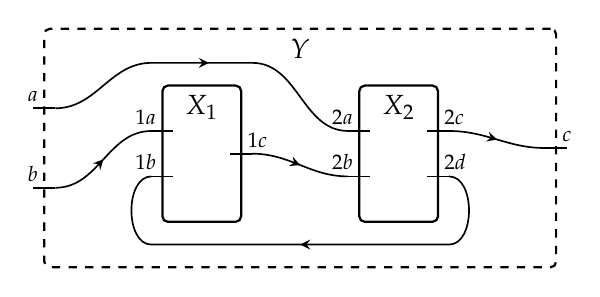
\begin{tikzpicture}[wiring diagram,baseline]
      \label{dia:string_diagram}
   \node[bb={2}{1}, bb name=$X_1$] (X1) {};
   \node[bb={2}{2}, right=of X1, bb name=$X_2$] (X2) {};
   \node[bb={2}{1}, dashed, fit={(X1) (X2) ($(X1.north)+(0,1.5)$) ($(X1.south)-(0,1)$)},
            bb name=$Y$] (Y) {};
   \draw[label]
      node[above left=of Y_in1]     {$a$}
      node[above left=of Y_in2]     {$b$}
      node[above right=of Y_out1]   {$c$}
      node[above left=of X1_in1]    {$1a$}
      node[above left=of X1_in2]    {$1b$}
      node[above right=of X1_out1]  {$1c$}
      node[above left=of X2_in1]    {$2a$}
      node[above left=of X2_in2]    {$2b$}
      node[above right=of X2_out1]  {$2c$}
      node[above right=of X2_out2]  {$2d$};
   \draw[ar] (Y_in2') to (X1_in1);
   \draw[ar] (X1_out1) to (X2_in2);
   \draw[ar] (X2_out1) to (Y_out1');
   \draw[ar] let \p1=(X1.north west), \p2=(X1.north east), \n1={\y1+\bby}, \n2=\bbportlen in
      (Y_in1') to (\x1-\n2,\n1) -- (\x2+\n2,\n1) to (X2_in1);
   \draw[ar] let \p1=(X2.south east), \p2=(X1.south west), \n1={\y1-\bby}, \n2=\bbportlen in
      (X2_out2) to[in=0] (\x1+\n2,\n1) -- (\x2-\n2,\n1) to[out=180] (X1_in2);
\end{tikzpicture}\end{equation}
represent compositions in a traced category $\cat{T}$. That is, new morphisms are constructed from old by specifying which outputs
will be fed back into which inputs. These are related to Penrose diagrams in $\ncat{Vect}$
and the word \emph{traced} originates in this vector space terminology~\cite{JoyalStreetVerity}.

The string diagrams of \cite{JoyalStreetVerity} typically do not explicitly include the outer box $Y$. If we include it, as in (\ref{dia:string_diagram}), the resulting \emph{wiring diagram} can be given a seemingly new interpretation: it represents a 1-dimensional cobordism between oriented 0-manifolds.  Indeed, the objects in $\Cob$ are signed sets $X=\inp{X}\sqcup\outp{X}$, each of which can be drawn as a box with input wires $\inp{X}$ entering on the left and output wires $\outp{X}$ exiting on the right. 
\begin{equation*}
   \begin{tikzpicture}[node distance=0 and 0, baseline=(current bounding box.center)]
      \node (A1) {$-$};
      \node[below=-.1 of A1] (A2) {$-$};
      \node[below=-.1 of A2] (A3) {$-$};
      \node[below=-.1 of A3] (B1) {$+$};
      \node[below=-.1 of B1] (B2) {$+$};
   \end{tikzpicture}
   \hspace{4em}
   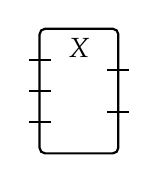
\begin{tikzpicture}[wiring diagram, bby=1.2ex, baseline=(current bounding box.center)]
      \node[bb={3}{2},bb name=$X$] {};
   \end{tikzpicture}
\end{equation*}
Moreover, the wiring diagram itself in which boxes $X_1,\ldots,X_n$ are wired together inside a larger box $Y$ can be interpreted as an oriented cobordism from $X_1\sqcup\cdots\sqcup X_n$ to $Y$.  In fact, this is more appropriately interpreted as a morphism in the (colored) operad $\Cob$ underlying the symmetric monoidal category of oriented 1-cobordisms.  

There is actually a bit more data in a string (or wiring) diagram for a traced category $\cat{T}$ than in a cobordism. Namely, each input and output of a box must be labeled by an object of $\cat{T}$ and the wires connecting boxes must respect the labels (e.g.\ in (\ref{dia:string_diagram}) objects $1c$ and $2b$ must be equal).  We will thus consider the operad $\LCob{\LabSet}$ of oriented 1-dimensional cobordisms over a fixed set of labels $\LabSet$. \todo[inline]{I would actually move the following sentence and diagram to the end of the previous paragraph, and remove the reference to $\LabSet$, since labels are not shown in the diagram.} The following shows the two approaches to drawing a 2-ary morphism $X_1,X_2\to Y$ in $\LCob{\LabSet}$:

\begin{equation*}
   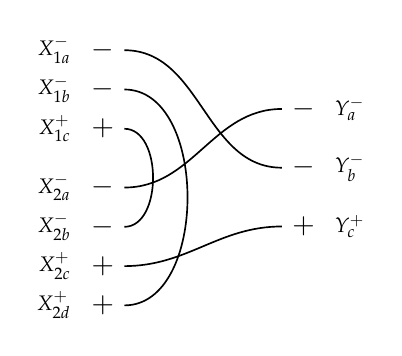
\begin{tikzpicture}[x=1cm,y=1ex,node distance=1 and 1,semithick,every label quotes/.style={font=\everymath\expandafter{\the\everymath\scriptstyle}},every to/.style={out=0,in=180},baseline=(current bounding box.center)]
      \node ["$\inp{X}_{1a}$" left] (X1a) {$-$};
      \node [below=0 of X1a, "$\inp{X}_{1b}$" left] (X1b) {$-$};
      \node [below=0 of X1b, "$\outp{X}_{1c}$" left] (X1c) {$+$};
      \node [below=1.5 of X1c, "$\inp{X}_{2a}$" left] (X2a) {$-$};
      \node [below=0 of X2a, "$\inp{X}_{2b}$" left] (X2b) {$-$};
      \node [below=0 of X2b, "$\outp{X}_{2c}$" left] (X2c) {$+$};
      \node [below=0 of X2c, "$\outp{X}_{2d}$" left] (X2d) {$+$};
      \node [below right=1.5 and 2 of X1a, "$\inp{Y}_a$" right] (Ya) {$-$};
      \node [below=1.5 of Ya, "$\inp{Y}_b$" right] (Yb) {$-$};
      \node [below=1.5 of Yb, "$\outp{Y}_c$" right] (Yc) {$+$};
      \draw (X1a) to (Yb);
      \draw (X1b) to[in=0] (X2d);
      \draw (X1c) to[in=0] (X2b);
      \draw (X2a) to (Ya);
      \draw (X2c) to (Yc);
   \end{tikzpicture}
   \qquad
   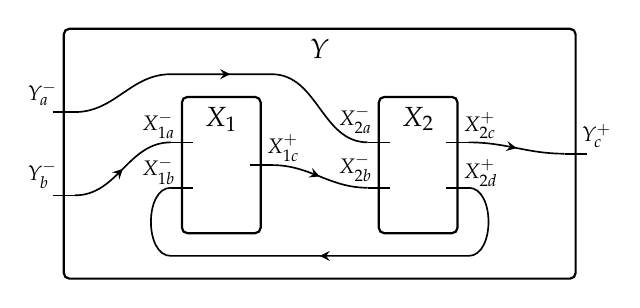
\begin{tikzpicture}[wiring diagram, baseline=(current bounding box.center)]
      \node[bb={2}{1}, bb name=$X_1$] (X1) {};
      \node[bb={2}{2}, right=of X1, bb name=$X_2$] (X2) {};
      \node[bb={2}{1}, fit={(X1) (X2) ($(X1.north)+(0,2)$) ($(X1.south)-(0,1)$)},bb name =$Y$] (Y) {};
      \draw[label]
          node[above left=of Y_in1]     {$\inp{Y}_a$}
          node[above left=of Y_in2]     {$\inp{Y}_b$}
          node[above right=of Y_out1]   {$\outp{Y}_c$}
          node[above left=1pt and -2pt of X1_in1]    {$\inp{X}_{1a}$}
          node[above left=1pt and -2pt of X1_in2]    {$\inp{X}_{1b}$}
          node[above right=1pt and -2pt of X1_out1]  {$\outp{X}_{1c}$}
          node[above left=3pt and -2pt of X2_in1]    {$\inp{X}_{2a}$}
          node[above left=2pt and -2pt of X2_in2]    {$\inp{X}_{2b}$}
          node[above right=1pt and -2pt of X2_out1]  {$\outp{X}_{2c}$}
          node[above right=0pt and -2pt of X2_out2]  {$\outp{X}_{2d}$};
      \draw[ar] (Y_in2') to (X1_in1);
      \draw[ar] (X1_out1) to (X2_in2);
      \draw[ar] (X2_out1) to (Y_out1');
      \draw[ar] let \p1=(X1.north west), \p2=(X1.north east), \n1={\y1+\bby}, \n2=\bbportlen in
          (Y_in1') to (\x1-\n2,\n1) -- (\x2+\n2,\n1) to (X2_in1);
      \draw[ar] let \p1=(X2.south east), \p2=(X1.south west), \n1={\y1-\bby}, \n2=\bbportlen in
         (X2_out2) to[in=0] (\x1+\n2,\n1) -- (\x2-\n2,\n1) to[out=180] (X1_in2);
   \end{tikzpicture}
\end{equation*}
In the table below, we record these two interpretations of a string diagram. Note the ``degree shift'' between the second and third columns.
\begin{center} \begin{tabular}{l|l|l}
   \toprule
      \multicolumn{3}{c}{Interpretations of string diagrams} \\
   \midrule
      String diagram & Traced category $\cat{T}$ & $\LCob{\LabSet}$ \\
   \midrule
      Wire label set, $\LabSet$ & Objects, $\LabSet\coloneqq\Ob(\cat{T})$ & Label set, $\LabSet$ \\
      Boxes, e.g.\ \tikz[wiring diagram,bb port sep=1,bby=2.4pt,bb min width=5.5pt,
                  bb port length=2pt,bb rounded corners=1pt,baseline=(B.south)]
               {\node[bb={1}{2}] (B) {};}
         & Morphisms in $\cat{T}$& Objects (oriented 0-mfds over $\LabSet$) \\
      String diagrams & Compositions in $\cat{T}$& Morphisms (cobordisms over $\LabSet$) \\
      Nesting & Axioms of traced cats & Composition (of cobordisms) \\
   \bottomrule
\end{tabular} \end{center}
In the last row above, each of the seven axioms of traced categories is vacuous from the cobordism perspective in the sense that both sides of the equation correspond to the same cobordism (up to diffeomorphism).  For example, the axiom of \emph{superposition} reads:
\[
   \Tr^U_{X,Y}\big[f\big]\otimes g=\Tr^U_{X\otimes W,Y\otimes Z}\big[f\otimes g\big]
\]
for every $f\colon U\otimes X\to U\otimes Y$ and $g\colon W\to Z$, or diagramatically:
\[\tikzset{bbx=.8cm,bb port sep=1.5}
   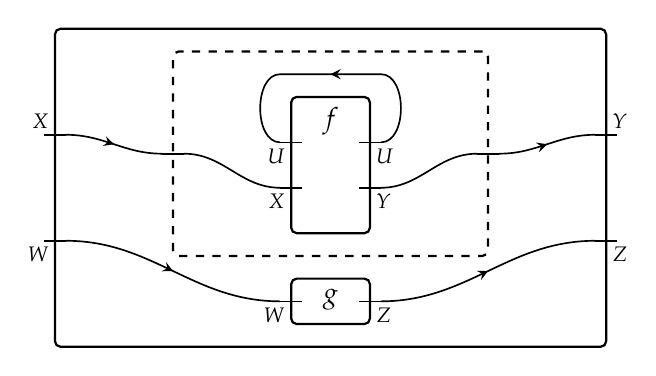
\begin{tikzpicture}[wiring diagram,baseline=(current bounding box.center)]
   \node[bb={2}{2}, bb name=$f$] (X1) {};
   \node[bb port sep=1,bb={1}{1}, below=2 of X1, bb name=$g$] (X2) {};
         \node[bb={1}{1}, fit={(X1) ($(X1.north)+(0,1)$)}, dashed] (Z) {};
         \node[bb={2}{2}, fit={(Z) (X2)}] (Y) {};
         \draw[ar] (Y_in1') to (Z_in1);
         \draw (Z_in1') to (X1_in2);
         \draw[ar] (Y_in2') to (X2_in1);
         \draw (X1_out2) to (Z_out1');
         \draw[ar] (Z_out1) to (Y_out1');
         \draw[ar] (X2_out1) to (Y_out2');
         \draw[ar] let \p1=(X1.north east), \p2=(X2.north west), \n1={\y1+\bby}, \n2=\bbportlen in
             (X1_out1) to[in=0] (\x1+\n2,\n1) -- (\x2-\n2,\n1) to[out=180] (X1_in1);
         \draw[label]
             node[above left=of Y_in1] {$X$}
             node[below left=of Y_in2] {$W$}
             node[above right=of Y_out1] {$Y$}
             node[below right=of Y_out2] {$Z$}
             node[below left=of X1_in1] {$U$}
             node[below left=of X1_in2] {$X$}
             node[below right=of X1_out2] {$Y$}
             node[below right=of X1_out1] {$U$}
             node[below left=of X2_in1] {$W$}
             node[below right=of X2_out1] {$Z$};
      \end{tikzpicture}
      \quad=\quad
      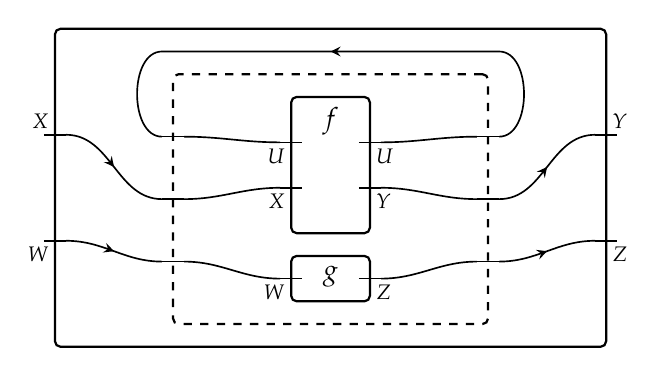
\begin{tikzpicture}[wiring diagram,baseline=(current bounding box.center)]
         \node[bb={2}{2}, bb name=$f$] (X1) {};
         \node[bb port sep=1,bb={1}{1}, below=of X1, bb name=$g$] (X2) {};
         \node[bb={3}{3}, fit={(X1) (X2)}, dashed] (Z) {};
         \node[bb={2}{2}, fit={(Z) ($(Z.north)+(0,1)$)}] (Y) {};
         \draw[ar] (Y_in1') to (Z_in2);
         \draw (Z_in2') to (X1_in2);
         \draw[ar] (Y_in2') to (Z_in3);
         \draw (Z_in3') to (X2_in1);
         \draw (X1_out2) to (Z_out2');
         \draw[ar] (Z_out2) to (Y_out1');
         \draw (X2_out1) to (Z_out3');
         \draw[ar] (Z_out3) to (Y_out2');
         \draw (Z_in1') to (X1_in1);
         \draw (X1_out1) to (Z_out1');
         \draw[ar] let \p1=(Z.north east), \p2=(Z.north west), \n1={\y1+\bby}, \n2=\bbportlen in
             (Z_out1) to[in=0] (\x1+\n2,\n1) -- (\x2-\n2,\n1) to[out=180] (Z_in1);
         \draw[label]
             node[above left=of Y_in1] {$X$}
             node[below left=of Y_in2] {$W$}
             node[above right=of Y_out1] {$Y$}
             node[below right=of Y_out2] {$Z$}
             node[below left=of X1_in1] {$U$}
             node[below left=of X1_in2] {$X$}
             node[below right=of X1_out2] {$Y$}
             node[below right=of X1_out1] {$U$}
             node[below left=of X2_in1] {$W$}
             node[below right=of X2_out1] {$Z$};
   \end{tikzpicture}
\]

To make precise the relationship between these interpretations of string diagrams, we fix the set $\LabSet$ of labels.  Let $\TrCat$ denote the 1-category of traced categories and traced strict monoidal functors.  Write $\TrCat_{\LabSet}$ for the subcategory in which the monoid of objects is fixed to be free on the set $\LabSet$, together with identity-on-objects functors.  
\begin{named}{Theorem 0}
   \label{th:traced is cob alg}
   There is an equivalence of 1-categories
   \begin{equation}
      \label{eq:single_fiber_tr}
      \LCob{\LabSet}\alg\equiv\TrCat_{\LabSet},
   \end{equation}
   where, given any monoidal category $\cat{M}$, we denote by $\cat{M}\alg\coloneqq\ncat{Lax}(\cat{M},\Set)$ the category of lax functors $\cat{M}\to\Set$.  
\end{named}
To build intuition for this statement note that the same data are required, and the same conditions are satisfied, whether one is specifying a lax functor $P\in\LCob{\LabSet}\alg$ or a traced category $\cat{T}\in\TrCat_{\LabSet}$ with objects freely generated by the set $\LabSet$.  First, for each box $X=(\inp{X},\outp{X})$ that might appear in a string diagram, both $P\colon\LCob{\LabSet}\to\Set$ and $\cat{T}$ require a set, $P(X)$ and $\Hom_{\cat{T}}(\inp{X},\outp{X})$, respectively.  Second, for each string diagram, both $P$ and $\cat{T}$ require a function: an action on morphisms in the case of $P$ and a formula for performing the required compositions, tensors, and traces in the case of $\cat{T}$. The condition that $P$ is functorial corresponds to the fact that $\cat{T}$ satisfies the axioms of traced categories.

We will briefly specify how to construct a lax functor $P$ from a traced category $(\cat{T},\otimes,I,\Tr)$ whose objects are freely generated by $\LabSet$. In what follows, we abuse notation slightly: given a relative set $\iota\colon Z\to\LabSet$ we will use the same symbol $Z$ to denote the tensor $\bigotimes_{z\in Z}\iota(z)$ in $\cat{T}$.  For an oriented 0-manifold $X=\inp{X}\sqcup \outp{X}$ over $\LabSet$, put $P(X)\coloneqq\Hom_{\cat{T}}(\inp{X},\outp{X})$. Given a cobordism $\Phi\colon X\to Y$, we need a function $P(\Phi)\colon P(X)\to P(Y)$. To specify it, note that for any cobordism $\Phi$ there exist $A,B,C,D,E\in\Ob(\cat{T})$ such that $\inp{X}\cong C\otimes A$, $\outp{X}\cong C\otimes B$, $\inp{Y}\cong A\otimes D$, $\outp{Y}\cong B\otimes D$, and $E$ is the set of floating loops in $\Phi$; thus $\Phi$ is essentially equivalent to the cobordism shown on the left side of (\ref{eq:cob_and_trace_pic}).
\begin{equation}
      \label{eq:cob_and_trace_pic}
   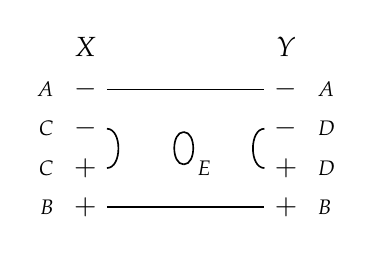
\begin{tikzpicture}[x=1cm,y=1ex,node distance=1 and 1,semithick,every label quotes/.style={font=\everymath\expandafter{\the\everymath\scriptstyle}},every to/.style={out=0,in=180},baseline=(current bounding box.center)]
      \node ["$A$" left] (X1a) {$-$};
      \node [above=0.25 of X1a] {$X$};
      \node [below=0 of X1a, "$C$" left] (X1b) {$-$};
      \node [below=0 of X1b, "$C$" left] (X2a) {$+$};
      \node [below=0 of X2a, "$B$" left] (X2b) {$+$};
      \node [right=2 of X1a, "$A$" right] (Y1a) {$-$};
      \node [above=0.25 of Y1a] {$Y$};
      \node [below=0 of Y1a, "$D$" right] (Y1b) {$-$};
      \node [below=0 of Y1b, "$D$" right] (Y2a) {$+$};
      \node [below=0 of Y2a, "$B$" right] (Y2b) {$+$};
      \node [right=1.45 of X2a, "$E$" left] {};
      \draw (X1a) to (Y1a);
      \draw (X1b) to[in=0] (X2a);
      \draw (X2b) to (Y2b);
      \draw (Y1b) to[in=180,out=180] (Y2a);
      \draw ($(X1b)+(1.25,-2.75)$) to[in=0] ($(X1b)+(1.25,-0.25)$);
      \draw ($(X1b)+(1.25,-0.25)$) to[in=180,out=180] ($(X1b)+(1.25,-2.75)$);
   \end{tikzpicture}
   \qquad\qquad
   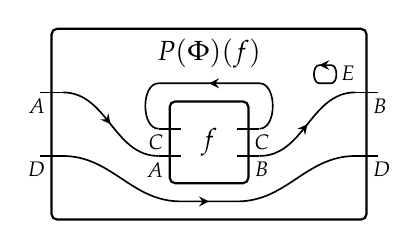
\begin{tikzpicture}[wiring diagram, bby=1.4ex, baseline=(current bounding box.center)]
      \node[bb port sep=1.5, bb={2}{2}] (domain) {$f$};
      \node[bb={2}{2}, fit={(domain) ($(domain.north)+(0,3)$) ($(domain.south)-(0,1)$)}, bb name=$P(\Phi)(f)$] (codomain) {};
      \draw[ar] (codomain_in1') to (domain_in2);
      \draw[ar] (domain_out2) to (codomain_out1');
      \draw[ar] let \p1=(domain.north east), \p2=(domain.north west), \n1={\y1+\bby}, \n2=\bbportlen in
          (domain_out1) to[in=0] (\x1+\n2,\n1) -- (\x2-\n2,\n1) to[out=180] (domain_in1);  %Trace on C
      \draw[ar] let \p1=(domain.south west), \p2=(domain.south east), \n1={\y1-\bby}, \n2=\bbportlen in
          (codomain_in2') to[in=180] (\x1+\n2,\n1) -- (\x2-\n2,\n1) to[out=0] (codomain_out2'); %Identity on D
      \draw[ar] let \p1=(domain.north east) in
          (\x1+.7*\bbx,\y1+\bby) to[in=0] (\x1+.7*\bbx,\y1+2*\bby) -- (\x1+.6*\bbx,\y1+2*\bby) to[out=180] (\x1+.6*\bbx,\y1+\bby) -- (\x1+.7*\bbx,\y1+\bby);%Loop
      \draw[label] let \p1=(domain.north east) in
          node[below left=of codomain_in1]     {$A$}
          node[below left=of codomain_in2]     {$D$}
          node[below right=of codomain_out1]    {$B$}
          node[below right=of codomain_out2]    {$D$}
          node[above left=.6 and 0 of codomain_out1']  {$E$}
          node[below left=of domain_in1]     {$C$}
          node[below left=of domain_in2]     {$A$}
          node[below right=of domain_out2]    {$B$}
          node[below right=of domain_out1]   {$C$};
   \end{tikzpicture}
\end{equation}
With the above notation, for $f\in P(X)$ we can follow the string diagram (right side of (\ref{eq:cob_and_trace_pic})) and define
\begin{equation}
      \label{eq:cob algebra formula}
   P(\Phi)(f)\coloneqq\Tr_{A,B}^C[f]\otimes D\otimes\Tr^E_{I,I}[E],
\end{equation}
where we abuse notation and write $D$ and $E$ for the identity maps on these objects.  One may easily check, using each axiom of the trace \cite{JoyalStreetVerity} in an essential way, that \eqref{eq:cob algebra formula} defines an algebra over $\LCob{\LabSet}$.  We will not prove \ref{th:traced is cob alg} directly as indicated here but to specify our proof strategy we must introduce more notation.


\section{The main results}
      \label{sec:main_results}

The equivalence \eqref{eq:single_fiber_tr} has two significant conceptual drawbacks: the object set of the traced category is fixed, and it is assumed to be freely generated by some set under tensor products; we refer to this latter condition using the term \emph{free-on-objects}. Much of the work in this paper goes towards relaxing these two conditions. 

To handle the free-on-objects condition, we prove that the 2-category of traced categories and strong functors is biequivalent to that of free-on-objects traced categories and strict functors; see Corollary~\ref{cor:object_frees}.  This result seems to be well-known to experts but is difficult to find in the literature.

To overcome the use of a fixed object set, we first explain what kind of object variance is appropriate.  There is an adjunction
\[\Adjoint{\Set}{\TrCat}{\FT}{\UT}\]
inducing a monad $\TT$ on $\Set$, which is in fact isomorphic to the free monoid monad.  Let $\cat{T}$ and $\cat{T}'$ be free-on-objects traced categories where $\Ob(\cat{T})$ is the free monoid on a set $\LabSet$ and $\Ob(\cat{T}')$ is the free monoid on a set $\LabSet'$. A strict (traced) monoidal functor $F\colon \cat{T}\to \cat{T}'$ induces a homomorphism $\Ob(F)\colon\Ob(\cat{T})\to\Ob(\cat{T}')$ between the free monoids, or equivalently a function $\Ob F\colon\LabSet\to\TT(\LabSet')$ which can be identified with a morphism in the Kleisli category $\Set_{\TT}$ of this monad.

Similarly, the compact category $\LCob{\LabSet}$ varies functorially in $\LabSet\in\Set$ and gives rise to a functor
\[(\LCob{\bullet})\colon\Set_{\TT}\to\CompCat\]
to the category $\CompCat$ of compact categories and strict functors, under which $\LabSet$ is sent to the free compact category on $\LabSet$ (e.g.\ see \cite{KellyLaplaza,Abramsky2}).  We can compose this with $\Lax(-,\Set)$ to obtain a functor which we denote
\begin{equation}
      \label{eqn:cob/bullet}
   (\LCob{\bullet})\alg\colon\Set_{\TT}^{\mathrm{op}}\too\Cat.
\end{equation}
By applying the Grothendieck construction (denoted by $\int$ here) to (\ref{eqn:cob/bullet}), we obtain a fibration for which the fiber over a set $\LabSet$ is equivalent (e.g.\ using \eqref{eq:single_fiber_tr}) to $\TrCat_{\LabSet}$.  Let $\TrFrObCat\subset\TrCat$ denote the full subcategory spanned by the traced categories that are free-on-objects.
\begin{named}{Theorem A}
      \label{thm:TheoremA_statement}
  There is an equivalence of 1-categories
  \begin{align*}
     &\int^{\LabSet\in\Set_{\TT}}(\LCob{\LabSet})\alg \to \TrFrObCat.
  \end{align*}
\end{named}
This result is proven in Section~\ref{sec:monoids_on_free} together with an analogous statement for compact categories.
\begin{remark}
   The most naive way of handling variation of the label set $\LabSet$ is to use plain functions $\LabSet\to\LabSet'$, rather than maps in the Kleisli category $\Set_{\TT}$. That is, instead of taking the Grothendieck construction of the functors \eqref{eqn:cob/bullet}, we could use the most evident functor $\Lax(\LCob{\bullet}\,,\Set)\colon\op{\Set}\to\Cat$. This would lead to a version of \ref{thm:TheoremA_statement} in which the right hand side is a 2-category of ``traced colored PROPs''. We will not pursue this direction in the paper; however, the interested reader familiar with PROPs should have no difficulty defining traced colored PROPs and proving the analogue of \ref{thm:TheoremA_statement} as a corollary of our results. For more on PROPs, see e.g.~\cite{HackneyRobertson}.
\end{remark}

In the course of proving \ref{thm:TheoremA_statement}, we will also establish a similar result which constructs the category of bijective-on-objects functors between traced categories.  To make this precise, we prove (Theorem~\ref{thm:orthogonal} and Proposition~\ref{prop:CompProf_exact}) that the well-known $(\bo,\ff)$ factorization system of $\Cat$ restricts to a factorization system on $\TrCat$; more precisely the left class consists of bijective-on-objects functors and the right class consists of fully faithful functors. 

Write $\TrCat^{\bo}$ for the full subcategory of the arrow category $\TrCat^{\to}$ spanned by the bijective-on-objects functors.  The existence of the factorization system implies that the domain functor
\[\dom\colon\TrCat^{\bo}\twoheadrightarrow\TrCat\]
is a fibration.  For a fixed traced category $\cat{T}$, the fiber $\TrCat^{\bo}_{\cat{T}/}\coloneqq\dom^{-1}(\cat{T})$ is the category of strict monoidal, bijective-on-objects functors from $\cat{T}$ to another traced category, with the evident commutative triangles as morphisms.  Note that we have an isomorphism $\TrCat_{\LabSet}\iso\TrCat^{\bo}_{(\FT\LabSet)/}$.

Recall from~\cite{JoyalStreetVerity} that traced categories can be thought of as full subcategories of compact categories: the Int construction applied to a traced category $\cat{T}$ returns the smallest compact category $\Int(\cat{T})$ of which $\cat{T}$ is a monoidal subcategory.  Generalizing \eqref{eq:single_fiber_tr}, we can give a complete characterization of lax functors out of such compact categories: for a fixed traced category $\cat{T}$ there is an equivalence of categories
\[\Lax(\Int(\cat{T}),\Set)\equiv\TrCat^{\bo}_{\cat{T}/}.\]
This is established in Section~\ref{sec:exactness_proofs} by proving the following generalization of \ref{thm:TheoremA_statement}.
\begin{named}{Theorem B}
      \label{thm:TheoremB_statement}
   There is an equivalence of fibrations
   \begin{equation*}
      \begin{tikzcd}[column sep=-1em]
         \int\limits^{\mathclap{\cat{T}\in\TrCat}} \Lax(\Int(\cat{T}),\Set)
               \ar[rr,"\equiv"] \ar[dr,two heads]
            && \TrCat^{\bo} \ar[dl,two heads,"\dom" pos=.4] \\
         & \TrCat. &
      \end{tikzcd}
   \end{equation*}
\end{named}

Our main tool in understanding this result will be the 2-categorical notion of \emph{(proarrow) equipments}, which we recall in Section~\ref{chap:background_equipments}. We will introduce what appears to be a new definition of \emph{monoidal profunctors}, and the equipment thereof, in Section\ref{chap:equipments_monoidal_profunctors}.

\erase{%%% begin erase %%%
\newpage

\section{Statements too general for intro that need to be placed somewhere}

Let $\TTrCat$ (resp.\ $\TTrCatStrong$) denote the 2-category of
traced categories, traced strict (resp.\ strong) monoidal functors, and monoidal natural isomorphisms
\cite{HK}, and let $\TrCat$ denote the underlying 1-category of $\TTrCat$%
\footnote{
   We use a similar notational convention throughout this paper. We denote named 1-categories,
   monoidal categories, and operads with bold roman letters, e.g., $\ncat{Cob}$, and unnamed
   1-categories with script, e.g., $\cat{C}$. For named 2-categories or bicategories we do almost
   the same, but change the font of the first letter to calligraphic, such as $\nncat{T}{rCat}$; for
   unnamed 2-categories we use (unbold) calligraphic, e.g., $\ccat{D}$.  Finally, for equipments
   (special double categories, see Section~\ref{chap:background_equipments}) we make the first
   letter blackboard bold, whether named (e.g., $\ndcat{P}{rof}$) or unnamed (e.g., $\dcat{D}$). The
   objects in a category, 2-category, or double category will be denoted with the usual math font
   (e.g., $T\in\Ob(\TrCat)$). By the \emph{underlying 1-category} of a 2-category, we mean the one
   obtained by dropping (not quotienting by) the 2-cells.
}.
Finally, let $\TrCat_{\LabSet}$ denote the subcategory in which the monoid of objects is fixed to be
free on the set $\LabSet$, together with identity-on-objects functors.


To state the next theorem, we give names to the categories described above. Let
\[
   \TTrFrObCat\ss\TTrCat \qquad \text{and} \qquad \CCompFrObCat\ss\CCompCat
\]
denote the full 2-subcategories spanned by the traced and compact categories (respectively) that are
free-on-objects. Let $\TrFrObCat$ and $\CompFrObCat$ (respectively) denote their underlying
1-categories.


\begin{named}{Theorem A}
      \label{thm:TheoremA_statement}
  There are equivalences of 1-categories
  \begin{align*}
     &\int^{\LabSet\in\Set_{\TT}}(\LCob{\LabSet})\alg \to \TrFrObCat
     \\
     &\int^{\LabSet\in\Set_{\TC}}(\LCob{\LabSet})\alg \to \CompFrObCat
  \end{align*}
\end{named}


Some intuition for this statement will be given in Section~\ref{subsec:cobalg_and_trCat}, and it
will be generalized in \ref{thm:TheoremA_statement} and proven as such in Section~\ref{sec:deducing}.

In order to see how the
free-on-objects traced (resp.\ compact) categories relate to general traced categories, we prove in
Appendix~\ref{appendix} the following result, which is well-known but difficult to find in the
literature:

\begin{corollary*}[\ref{cor:object_frees}]
   The canonical inclusions
   \begin{align*}
      \MMonFrObCat &\to \MMonCatStrong \\
      \TTrFrObCat &\to \TTrCatStrong \\
      \CCompFrObCat &\to \CCompCatStrong
   \end{align*}
   are biequivalences of 2-categories.
\end{corollary*}

Here $\MMonFrObCat$ and $\MMonCatStrong$ are defined analogously to the other two. See
Definition~\ref{def:free_on_objects}.



Our work in this direction leads to a characterization (see
Remark~\ref{rem:characterization_of_traced}) of the 2-category $\TTrCatStrong$ solely in terms of
$\MMonCatStrong$ and $\CCompCatStrong$---and the relationship between them---without mention of the
usual structures or axioms of traced categories as in \cite{JoyalStreetVerity}.

\subsection{Compact categories vs.\ traced categories}

For each of our main results about traced categories in this paper, we will also prove an analogous
result about compact closed symmetric monoidal categories, hereafter \emph{compact categories}. The
definition of compact category can be found in Section~\ref{sec:compact_and_int}, or
in~\cite{MacL--CTWM}. Let $\CCompCat$ (resp.\ $\CCompCatStrong$) denote the 2-category of compact
categories with strict (resp.\ strong) functors, and let $\CompCat$ denote the underlying 1-category
of $\CCompCat$. As above, let $\CompCat_{\LabSet}$ denote the subcategory of compact categories
whose objects are free on the set $\LabSet$ (so the objects are strings such as $o_1o_2o_3^*$ of
labels $o_i\in\LabSet$ and their formal duals, and the tensor product is concatenation), together
with identity-on-objects functors.

There is an equivalence of categories
\begin{equation}
      \label{eq:single_fiber_comp}
   \LCob{\LabSet}\alg\equiv\CompCat_{\LabSet}.
\end{equation}
Equations \eqref{eq:single_fiber_tr} and \eqref{eq:single_fiber_comp} and the relationship between
them will be generalized in \ref{thm:TheoremA_statement}; see also \eqref{eqn:2pullbacks_1fiber}.


\subsection{compact categories statements from subsection~\ref{sec:main_results}}

\[
   \qquad\text{and}\qquad
   \Adjoint{\Set}{\CompCat}{\FC}{\UC}
\]
 Likewise, if $\cat{C}$ and $\cat{C}'$ are free-on-objects compact categories, then the object part $\Ob F$ of a strong functor $F\colon\cat{C}\to\cat{C}'$ can be identified with a morphism in the Kleisli category $\Set_{\TC}$.

 \[\qquad\text{and}
   \qquad
   (\LCob{\bullet})\colon\Set_{\TC}\to\CompCat
\]

\begin{equation}
   \qquad\text{and}\qquad
   (\LCob{\bullet})\alg\colon\Set_{\TC}^{\mathrm{op}}\too\Cat.
\end{equation}

\[
   \qquad\text{and}\qquad
   \dom\colon\CompCat^{\bo}\twoheadrightarrow\CompCat
\]

\begin{equation}
   \qquad\text{and}\qquad
   \Lax(\cat{C},\Set)\equiv\CompCat^{\bo}_{\cat{C}/}.
\end{equation}

\begin{equation*}
      \qquad\text{and}\qquad
      \begin{tikzcd}[column sep=-1em]
         \int\limits^{\mathclap{\cat{C}\in\CompCat}} \Lax(\cat{C},\Set)
               \ar[rr,"\equiv"] \ar[dr,two heads]
            && \CompCat^{\bo} \ar[dl,two heads,"\dom" pos=.4] \\
         & \CompCat &
      \end{tikzcd}
\end{equation*}

}%%% end erase %%%


\section{Plan of the paper}
\todo[inline]{Make sure this plan is still correct.}

Section~\ref{sec:equipments} reviews the notion of an equipment (or framed bicategory \cite{Shulman}).  In Section~\ref{sec:internal_presheaves} we record the definition of copresheaves internal to an equipment which will allow us to reformulate and properly understand our main theorems. Section~\ref{sec:monoids_bimods} recalls monoids and bimodules in an equipment and establishes basic facts and constructions needed for the main theorems; in particular, exact equipments \cite{Schultz2015} are defined using this language.  In Section~\ref{sec:monoidal,compact,traced} we review monoidal, traced, and compact categories. We finally introduce various equipments of monoidal profunctors ($\dMonProf, \dTrProf$, and $\dCompProf$) at the heart of the paper in Section~\ref{sec:monoidal_profunctors}.   In Section~\ref{sec:special_CompProf} we prove the special properties about $\dCompProf$ which are at the core of our results.  Indeed one might view the rest of the paper as a formal wrapper for the results in that section.  In Section~\ref{sec:exactness_proofs} we prove that the equipments of interest are exact and then apply the theory developed in Section~\ref{chap:background_equipments} to deduce \ref{thm:TheoremB}.  In Section~\ref{sec:monoids_on_free} we deal with the freeness-on-objects needed for \ref{thm:TheoremA}. The appendix contains material that is not necessary to the paper. Its function is to prove the biequivalence between the 2-category $\MMonCatStrong$ of monoidal categories with arbitrary object set and strong functors, on the one hand, and the 2-category $\MMonFrObCat$ of monoidal categories with free object set and strict functors. We do the same for traced and compact categories, all in Corollary~\ref{cor:object_frees}.

\section*{Acknowledgments}

Thanks go to Steve Awodey and Ed Morehouse for suggesting we formally connect the operad-algebra
picture in \cite{RupelSpivak} to string diagrams in traced categories. We also thank Mike Shulman
for many useful conversations, and Tobias Fritz, Justin Hilburn, and Dmitry Vagner for helpful
comments on drafts of this paper. Finally, we thank our referee for many useful suggestions.


\chapter{Background on equipments}
      \label{chap:background_equipments}

This section introduces equipments, which we use to properly situate traced and compact categories.
This tool will eventually allow us to clarify the relationship between strict monoidal functors
between monoidal categories and lax monoidal functors to $\Set$.

\section{Equipments}
   \label{sec:equipments}

A double category is a 2-category-like structure involving horizontal and vertical arrows, as well
as 2-cells. An equipment (sometimes called a \emph{proarrow equipment} or \emph{framed bicategory})
is a double category satisfying a certain fibrancy condition. In this section, we will spell this
out and give two relevant examples. An excellent reference is Shulman's paper \cite{Shulman}; see also
\cite{Wood1} and \cite{Wood2}.

\begin{definition}
   A \emph{double category} $\dcat{D}$\footnote{We will use many flavors of category in this paper. To help distinguish, we denote named 1-categories, monoidal categories, and operads with bold roman letters, e.g.\ $\ncat{Cob}$, and unnamed 1-categories with script, e.g.\ $\cat{C}$. For named 2-categories or bicategories we do almost the same, but change the font of the first letter to calligraphic, such as $\nncat{T}{rCat}$; for unnamed 2-categories we use (unbold) calligraphic, e.g.\ $\ccat{D}$.  Finally, for double categories we make the first letter blackboard bold, whether named (e.g., $\ndcat{P}{rof}$) or unnamed (e.g., $\dcat{D}$). The objects in a category, 2-category, or double category will be denoted with the usual math font (e.g.\ $T\in\Ob\TrCat$ or $c\in\Ob\dcat{D}$).} consists of the following data:
   \begin{itemize}
      \item A category $\dcat{D}_0$, which we refer to as the \emph{vertical category} of
         $\dcat{D}$. For any two objects $c,d\in\dcat{D}_0$, we will write
         $\dcat{D}_0(c,d)$ for the set of vertical arrows from $c$ to $d$. We refer to
         objects of $\dcat{D}_0$ as objects of $\dcat{D}$.
      \item A category $\dcat{D}_1$, equipped with two functors $\lframe,\rframe\colon\dcat{D}_1\to\dcat{D}_0$,
         called the \emph{left frame} and \emph{right frame} functors. Given an object
         $M\in\Ob(\dcat{D}_1)$ with $c=\lframe(M)$ and $c'=\rframe(M)$, we say that $M$ is a \emph{proarrow} (or
            \emph{horizontal arrow}) \emph{from $c$ to $c'$} and write $M\colon c\tickar c'$. A
            morphism $\phi\colon M\to N$ in $\dcat{D}_1$ is called a 2-cell, and is drawn as
            follows, where $f=\lframe(\phi)$ and $f'=\rframe(\phi)$:
         \begin{equation} \begin{tikzcd}
               \label{eqn:2cell}
            c \ar[r,tick,"M" domA] \ar[d,"f"']
            & c'\ar[d,"f'"]
              \\
            d \ar[r,tick,"N"' codA]
              & d'
            \twocellA{\phi}
         \end{tikzcd} \end{equation}
      \item A \emph{unit} functor $\unit\colon\dcat{D}_0\to\dcat{D}_1$, which is a
         section of both $\lframe$ and $\rframe$, i.e.\ $\lframe\circ\unit=\id_{\dcat{D}_0}=\rframe\circ\unit$. We will often
         abuse notation by writing $c$ for the unit proarrow $\unit(c)\colon c\tickar c$, and similarly
         for vertical arrows.
      \item A functor $\odot\colon\dcat{D}_1\times_{\dcat{D}_0}\dcat{D}_1\to\dcat{D}_1$, called
         \emph{horizontal composition}, that is weakly associative and unital in the sense that
         there are coherent unitor and associator isomorphisms. See \cite{Shulman} for more details.
   \end{itemize}
   Given a double category $\dcat{D}$ there is a strict 2-category called the \emph{vertical
   2-category}, denoted $\VVer(\dcat{D})$, whose underlying 1-category\footnote{By the \emph{underlying 1-category} of a 2-category, we mean the one obtained by dropping (not quotienting by) the 2-cells.} is $\dcat{D}_0$ and whose 2-morphisms $f\Rightarrow f'$ are defined to be 2-cells \eqref{eqn:2cell} where $M=\unit(c)$ and $N=\unit(d)$ are unit proarrows. There is also a \emph{horizontal bicategory}, denoted $\HHor(\dcat{D})$, whose objects and 1-cells are the objects and horizontal 1-cells of
   $\dcat{D}$ and whose 2-cells are the 2-cells of $\dcat{D}$ of the form \eqref{eqn:2cell} such that $f=\id_c$ and $f'=\id_{c'}$.

   A \emph{strong double functor} $F\colon\dcat{C}\to\dcat{D}$ consists of functors
   $F_0\colon\dcat{C}_0\to\dcat{D}_0$ and $F_1\colon\dcat{C}_1\to\dcat{D}_1$ commuting with the frames $\lframe$,$\rframe$, and
   preserving the unit $\unit$ and horizontal composition $\odot$ up to coherent isomorphism.
\end{definition}

\begin{definition}
      \label{def:equipment}
   An \emph{equipment} is a double category $\dcat{D}$ in which the frame functor
   \[
      (\lframe,\rframe)\colon\dcat{D}_1\onto\dcat{D}_0\times\dcat{D}_0
   \]
   is a fibration. If $f\colon c\to d$ and $f'\colon c'\to d'$ are vertical morphisms and $N\colon
   d\tickar d'$ is a proarrow, a cartesian morphism $M\to N$ in $\dcat{D}_1$ over $(f,f')$ is a
   2-cell
   \[ \begin{tikzcd}
      c \ar[r,tick, "M" domA] \ar[d,"f"']
         & c'\ar[d,"f'"] \\
      d \ar[r,tick,"N"' codA]
         & d'
      \twocellA{\tn{cart}}
   \end{tikzcd} \]
   which we call a \emph{cartesian 2-cell}. We refer to $M$ as the \emph{restriction of $N$ along
   $f$ and $f'$}, written $M=N(f',f)$.  
\end{definition}

\begin{definition}
      \label{def:local_equivalence}
   By an \emph{equipment functor}, we simply mean a strong double functor between equipments.  We refer to an equipment functor $F\colon\dcat{C}\to\dcat{D}$ as a \emph{local equivalence} if the following square strictly commutes and is a pseudo-pullback of categories:
   \begin{equation} \begin{tikzcd}
         \label{eqn:local_equiv}
      \dcat{C}_1 \ar[r,"F_1"] \ar[d,two heads,"{(\lframe,\rframe)}"'] \ar[dr,phantom,"\lrcorner" very near start]
         & \dcat{D}_1 \ar[d,two heads,"{(\lframe,\rframe)}"] \\
      \dcat{C}_0\times\dcat{C}_0 \ar[r,"F_0\times F_0"']
         & \dcat{D}_0\times\dcat{D}_0.
   \end{tikzcd} \end{equation}
   If moreover $F_0\colon\dcat{C}_0\to\dcat{D}_0$ is fully faithful, we say that $F$ is a \emph{fully faithful local equivalence}.
\end{definition}

\begin{remark}
      \label{rem:strict_vs_pseudo_pullback}
   It is a standard fact for 1-categories that a strict pullback of an isofibration along an arbitrary functor is a pseudo-pullback. Any Grothendieck fibration (or opfibration) is in particular an isofibration, so the square \eqref{eqn:local_equiv} being a strict pullback implies it is also a pseudo-pullback.

   Also note that the frame fibration for $\dcat{C}$ is equivalent to the functor $\dcat{C}_0\times\dcat{C}_0\to\CCat$, the 2-category of
   small categories, sending $(c,d)$ to $\HHor(\dcat{C})(c,d)$ and similarly for $\dcat{D}$.  In this language, $F$ is a local equivalence if and only if the induced functors $\HHor(\dcat{C})(c,d)\to\HHor(\dcat{D})(F_0(c),F_0(d))$ are equivalences of categories for every pair of objects $(c,d)$. The square \eqref{eqn:local_equiv} is a strict pullback precisely when these are isomorphisms of categories.
\end{remark}

\begin{definition}
      \label{def:induced_locally_equivalent_equipment}
   Let $\dcat{D}$ be a double category and $F_0\colon\dcat{C}_0\to\dcat{D}_0$ be a functor. A strict pullback of the form \eqref{eqn:local_equiv} defines a double category $\dcat{C}$, which we denote
   \[
      \dcat{C}\coloneqq F_0^*(\dcat{D}).
   \]
   If $\dcat{D}$ is an equipment, $F_0^*(\dcat{D})$ will be as well since fibrations are stable under pullback. In this case we call $F_0^*(\dcat{D})$ the \emph{equipment induced by $F_0$}. By Remark~\ref{rem:strict_vs_pseudo_pullback}, the induced equipment functor $F_0^*(\dcat{D})\to\dcat{D}$ is a local equivalence.
\end{definition}

\begin{example}
      \label{ex:dspan}
   There is an equipment $\dSpan$ of spans in $\Set$. Its vertical category is
   $\dSpan_0\coloneqq\Set$. A horizontal 1-cell between sets $A$ and $B$ is a span $A\from S\to B$,
   their composition is defined by a pullback of spans, and a 2-cell in $\dSpan$ is a commutative
   diagram in $\Set$ of the appropriate shape. A cartesian 2-cell in this equipment is obtained by
   taking an evident limit in $\Set$.
\end{example}

Our main tool in this paper will be equipments of profunctors as in the following example.
\begin{example}\label{ex:profunctors}
   The equipment $\dProf$ is a double category whose vertical category $\dProf_0=\Cat$ is the category of small 1-categories and
   functors.  Given categories $\cat{C},\cat{C}'\in\dProf_0$, a proarrow 
   \[ \begin{tikzcd}
      \cat{C} \ar[r,tick,"M"] & \cat{C}'
   \end{tikzcd} \]
   in $\dProf_1$ is a profunctor, that is a functor $M\colon\op{\cat{C}}\times\cat{C}'\to\Set$.  The left and right frame functors are given by $L(M)=\cat{C}$ and $R(M)=\cat{C}'$.  A 2-cell $\phi$ in $\dProf$, as to the left, denotes a natural transformation, as to the right, in \eqref{eqn:Prof2cells}:
   \begin{equation}
         \label{eqn:Prof2cells}
      \begin{tikzcd}
         \cat{C} \ar[r,tick,"M" domA] \ar[d,"F"']
            & \cat{C}'\ar[d,"F'"] \\
         \cat{D} \ar[r,tick,"N"' codA]
            & \cat{D}'
         \twocellA{\phi}
      \end{tikzcd}
      \hspace{.6in}
      \begin{tikzcd}[column sep=.8em, row sep=5ex]
         \op{\cat{C}}\times \cat{C}' \ar[dr,"M"'] \ar[rr,"\op{F}\times F'"]
            & \ar[d,phantom,"\overset{\phi}{\Rightarrow}" near start]
            & \op{\cat{D}}\times \cat{D}'\ar[dl,"N"] \\
         & \Set.
      \end{tikzcd}
   \end{equation}
   For any category $\cat{C}\in\dProf_0$, $\Hom_{\cat{C}}\colon\op{\cat{C}}\times\cat{C}\to\Set$ is a profunctor and $U(\cat{C})=\Hom_{\cat{C}}$ is the unit functor of $\dProf$.  Given two profunctors
   \[ \begin{tikzcd}
      \cat{C} \ar[r,tick,"M"] & \cat{D} \ar[r,tick,"N"] & \cat{E},
   \end{tikzcd} \]
   define the horizontal composition $M\odot N$ on objects $c\in\cat{C}$ and $e\in\cat{E}$ as the coequalizer of the diagram
   \begin{equation} \begin{tikzcd}
      \label{eqn:coendComp}
      \displaystyle\coprod_{d_1,d_2\in\cat{D}} M(c,d_1)\times\cat{D}(d_1,d_2)\times N(d_2,e)
         \ar[r,shift left] \ar[r,shift right]
      & \displaystyle\coprod_{d\in\cat{D}} M(c,d)\times N(d,e)
   \end{tikzcd} \end{equation}
   where the two maps are given by the right and left actions of $\cat{D}$ on $M$ and $N$ respectively. We can write elements of $(M\odot N)(c,e)$ as tensors $m\otimes n$, where $m\in M(c,d)$ and $n\in N(d,e)$ for some $d\in\cat{D}$. The construction as a coequalizer then implies that $(m\cdot f)\otimes n=m\otimes(f\cdot n)$ whenever the equation makes sense.  Note that the coequalizer \eqref{eqn:coendComp} is in fact a reflexive coequalizer, using $\id_b\in\cat{B}(b,b)$.  Given a profunctor $M:\cat{C}\tickar\cat{C'}$ there are canonical isomorphisms $\Hom_{\cat{C}}\odot M \iso M \iso M\odot\Hom_{\cat{D}}$ which can be viewed as giving an action of $\Hom_{\cat{C}}$ and of $\Hom_{\cat{D}}$ on $M$ from the left and right respectively.

   Together these give $\dProf$ the structure of a double category.  To see that $\dProf$ is an equipment, note that from a pair of functors $F\colon\cat{C}\to\cat{D}$, $F'\colon\cat{C}'\to\cat{D}'$ and a profunctor $N\colon \cat{D}\tickar\cat{D}'$ we may form the composite 
   \[\begin{tikzcd}
      \op{\cat{C}}\times\cat{C}' \ar[r,"\op{F}\times F'"]
         &[1.5em] \op{\cat{D}}\times\cat{D}' \ar[r,"N"]
         & \Set,
   \end{tikzcd}\]
   denoted $N(F',F):\cat{C}\tickar\cat{C}'$, such that
   \begin{equation}
      \label{eq:cartesian profunctor morphism}
      \begin{tikzcd}
      \cat{C} \ar[r,tick,"{N(F',F)}" domA] \ar[d,"F"']
         & \cat{C}'\ar[d,"F'"] \\
      \cat{D} \ar[r,tick,"N"' codA]
         & \cat{D}'
      \twocellA{\phi}
      \end{tikzcd}
   \end{equation}
   is a cartesian 2-cell.  Note that an easy Yoneda lemma argument yields $\VVer(\dProf)\equiv\CCat$.
\end{example}
%An equipment $\dcat{D}$ is often named according to its horizontal arrows. In Example~\ref{ex:profunctors} we discussed profunctors, which are the horizontal arrows in an equipment $\dProf$. Variations on $\dProf$, such as $\dMonProf, \dTrProf,$ and $\dCompProf$ (defined in Section~\ref{sec:monoidal_profunctors}) will play a major role in this paper.


\section{Internal copresheaves}
      \label{sec:internal_presheaves}

Copresheaves on a category $\cat{C}$ can be identified with profunctors $\cat{C}\tickar1$ in $\dProf$. Motivated by this, we will think of
proarrows $c\tickar 1$ in any equipment $\dcat{D}$ with a terminal object 1 as ``internal
copresheaves'' on the object $c$.  For each object, there is a category of copresheaves
$\HHor(\dcat{D})(c,1)$.  We can give a direct construction of the bifibration over $\dcat{D}_0$ whose
fiber over an object $c$ is the category of copresheaves on $c$:

\begin{definition}
      \label{def:copresheaves}
   Let $\dcat{D}$ be an equipment with a terminal object $1\in\dcat{D}_0$.%
   \footnote{In fact, such a definition makes sense for any object of $\dcat{D}_0$, but for our
   purposes we require the terminal object.}
   We define the category $\CPsh(\dcat{D})$, bifibered over
   $\dcat{D}_0$, by the strict pullback of categories
   \begin{equation*}
     \begin{tikzcd}
         \CPsh(\dcat{D}) \ar[r] \ar[d,two heads] \arrow[dr,phantom,"\lrcorner",very near start]
            & \dcat{D}_1 \ar[d,two heads] \\
         \dcat{D}_0\times 1 \ar[r,"\dcat{D}_0\times 1"']
            & \dcat{D}_0\times\dcat{D}_0.
      \end{tikzcd}
   \end{equation*}
\end{definition}

\begin{lemma}
      \label{lem:Psh_pullback}
   Let $F\colon\dcat{C}\to\dcat{D}$ be an equipment functor. Suppose that $\dcat{C}_0$ and
   $\dcat{D}_0$ have terminal objects preserved by $F$. Then there is an induced
   morphism of fibrations
   \begin{equation} \begin{tikzcd}
         \label{eq:CPsh_square}
      \CPsh(\dcat{C}) \ar[r,"\tilde{F}"] \ar[d,two heads] % \ar[dr,phantom,"\lrcorner" very near start]
         & \CPsh(\dcat{D}) \ar[d,two heads] \\
      \dcat{C}_0 \ar[r,"F_0"']
         & \dcat{D}_0.
   \end{tikzcd} \end{equation}
   Moreover, if $F$ is a local equivalence, then~\eqref{eq:CPsh_square} is a pseudo-pullback.
\end{lemma}
\begin{proof}
   Consider the cube
   \[ \begin{tikzcd}[row sep={40,between origins}, column sep={55,between origins}]
      \CPsh(\dcat{C}) \ar[rr,"\tilde{F}"] \ar[dr] \ar[dd,two heads]
      &[-10] & \CPsh(\dcat{D}) \ar[dd,two heads] \ar[dr] &[-10] \\[-5]
      & \dcat{C}_1 \ar[rr,crossing over,"F_1" near start]
         && \dcat{D}_1 \ar[dd,two heads] \\
      \dcat{C}_0\times 1 \ar[rr,"F_0\times 1" pos=.75]
            \ar[dr,"\id\times 1"' {pos=.25,inner sep=2pt}]
         && \dcat{D}_0\times 1 \ar[dr,"\id\times 1"' {pos=.25,inner sep=2pt}] & \\[-5]
      & \dcat{C}_0\times\dcat{C}_0 \ar[rr,"F_0\times F_0"']
            \ar[from=uu,crossing over,two heads]
         && \dcat{D}_0\times\dcat{D}_0.
   \end{tikzcd} \]
   Since $F_0$ preserves terminal objects, the bottom face of the cube commutes. The left and right faces of
   the cube are strict pullbacks by definition, hence there is a unique $\tilde{F}$ making the cube commute.

   If $F$ is a local equivalence, then the front face is a pseudo-pullback. The left and right faces
   are strict pullbacks along fibrations, hence pseudo-pullbacks (see Remark~\ref{rem:strict_vs_pseudo_pullback}).  It follows that the
   back face is a pseudo-pullback as well.
\end{proof}
\erase{%begin erase
\begin{example}
If $\dcat{D}=\dProf$ then an object of $\CPsh(\dcat{D})$ is a pair $(\cat{C},H)$, where $\cat{C}$ is a category
and $H\colon \cat{C}\to\Set$ is a functor. A morphism $(\cat{C},H)\to(\cat{C}',H')$ is a pair $(F,F^\sharp)$ of a
functor and a natural transformation, as in the lax triangle
\[ \begin{tikzcd}[column sep=.6cm]
   \cat{C}\ar[rr,"F"]\ar[rd,"H"']&\ar[d,phantom,"\overset{F^\sharp}{\Rightarrow}" near start]&\cat{C}'\ar[dl,"H'"]\\
   &\Set.
\end{tikzcd} \]
\end{example}}%end erase


\section{Monoids and bimodules}
      \label{sec:monoids_bimods}

Our eventual proofs of Theorems A and B will revolve around a careful understanding of internal monoids in an equipment $\dcat{D}$.  In particular, following~\cite{Schultz2015}, the exactness of an equipment given in Definition~\ref{def:exact_equipment} and the $(\bo,\ff)$ factorization system given in Theorem~\ref{thm:orthogonal} are built on notions related to monoids in $\dcat{D}$.
\begin{definition}
      \label{def:monoids}
   Denote by $\Mon(\dcat{D})$ the category of monoids in $\dcat{D}$.  More precisely, the objects are \emph{monoids}: tuples $(c,M,i_M,m_M)$ consisting of an object $c$ of $\dcat{D}$ and a proarrow $M\colon c\tickar c$ together with unit and multiplication cells
   \begin{equation}
      \label{eqn:unit_and_mult}
      \begin{tikzcd}
         c \ar[r,tick,"c" domA] \ar[d,equal]
            & c \ar[d,equal] \\
         c \ar[r,tick,"M"' codA] & c
         \twocellA{i_M}
      \end{tikzcd}
      \qquad
      \begin{tikzcd}
         c \ar[r,tick,"M"] \ar[d,equal]
            & |[alias=domA]| c \ar[r,tick,"M"]
            & c \ar[d,equal] \\
         c \ar[rr,tick,"M"' codA]
            && c
         \twocellA{m_M}
      \end{tikzcd}
   \end{equation}
   satisfying the evident unit and associativity axioms.  The morphisms are \emph{monoid homomorphisms}: pairs $(f,\vec{f}\mspace{2mu})$ consisting of a vertical arrow $f\colon c\to d$ in $\dcat{D}$ and a cell
   \[ \begin{tikzcd}
         c \ar[r,tick,"M" domA] \ar[d,"f"']
            & c \ar[d,"f"] \\
         d \ar[r,tick,"N"' codA]
            & d
         \twocellA{\vec{f}}
      \end{tikzcd} \]
   which respects the unit and multiplication cells of $M$ and $N$.
\end{definition}

There is an evident forgetful functor $\MOb\colon\Mon(\dcat{D})\to\dcat{D}_0$ sending a monoid $M\colon c\tickar c$ to its underlying object $c=|M|$.  
\begin{lemma}
   Let $\dcat{D}$ be an equipment.  The forgetful functor $\MOb\colon\Mon(\dcat{D})\to\dcat{D}_0$ is a
   fibration and there is a morphism of fibrations
   \[ \begin{tikzcd}[column sep=tiny]
      \Mon(\dcat{D}) \ar[d,two heads,"\MOb"'] \ar[r]
         & \dcat{D}_1 \ar[d,two heads] \\
      \dcat{D}_0 \ar[r,"\Delta"']&\dcat{D}_0\times\dcat{D}_0.
   \end{tikzcd} \]
\end{lemma}
\begin{proof}
   Let $f\colon c\to d$ be a vertical morphism of $\dcat{D}$ and $N\colon d\tickar d$ a monoid in $\dcat{D}$.  Since the 2-cell defining the restriction of $N$ along $f$ is cartesian, there is an induced monoid structure on $N(f,f)$ which in particular makes this cartesian 2-cell a monoid homomorphism.  The result follows.
\end{proof}

\begin{lemma}
      \label{lem:Mon_pullback}
   For a local equivalence $F\colon\dcat{C}\to\dcat{D}$, the induced square
   \[ \begin{tikzcd}
      \Mon(\dcat{C}) \ar[r,"\Mon(F)"] \ar[d,two heads,"\MOb"'] \ar[dr,phantom,"\lrcorner" very near start]
         & \Mon(\dcat{D}) \ar[d,two heads,"\MOb"] \\
      \dcat{C}_0 \ar[r,"F_0"']
         & \dcat{D}_0
   \end{tikzcd} \]
   is a pseudo-pullback of categories.  
\end{lemma}
\begin{proof}
   We may assume without loss of generality that the pullback in Definition~\ref{def:local_equivalence} realizing $F\colon\dcat{C}\to\dcat{D}$ as a local equivalence is strict.  It is then straightforward to check directly that the above square is again a strict pullback and hence a pseudo-pullback following Remark~\ref{rem:strict_vs_pseudo_pullback}.
\end{proof}

\begin{definition}
      \label{def:embedding}
   Let $M\colon c\tickar c$ be a monoid in an equipment $\dcat{D}$. An \emph{embedding} of $M$ into
   an object $x\in\dcat{D}_0$ is a monoid homomorphism $(f,\vec{f}\mspace{2mu})$ from $M$ to the trivial monoid on $x$:
   \[ \begin{tikzcd}
      c \ar[r,tick,"M" domA] \ar[d,"f"']
         & c \ar[d,"f"] \\
      x \ar[r,tick,"x"' codA]
         & x.
      \twocellA{\vec{f}}
   \end{tikzcd} \]
   We will sometimes write an embedding as $(f,\vec{f}\mspace{2mu})\colon(c,M)\to x$, or even just $f\colon M\to
   x$ when clear from context. We will write $\Emb(M,x)$ for the set of embeddings from $M$ to $x$.
   This defines a functor $\Emb\colon\op{\Mon(\dcat{D})}\times\dcat{D}_0\to\Set$.
\end{definition}

\begin{lemma}
      \label{lemma:embed_for_LE}
   Suppose that $F\colon\dcat{C}\to\dcat{D}$ is a local equivalence induced by
   $F_0\colon\dcat{C}_0\to\dcat{D}_0$. Suppose $M\in\Mon(\dcat{C})$ is a monoid and $x\in\dcat{C}_0$
   is an object.  For $N=\Mon(F)(M)$ and $y=F_0(x)$ we have a pullback square in $\Set$, natural in
   $M$ and $x$:
      \[ \begin{tikzcd}
         \Emb_{\dcat{C}}(M,x)\ar[r]\ar[d]\ar[rd,phantom,"\lrcorner" very near start]
         &\Emb_{\dcat{D}}(N,y)\ar[d]
         \\
         \dcat{C}_0(|M|,x)\ar[r]
         &\dcat{D}_0(|N|,y).
      \end{tikzcd} \]
\end{lemma}

\begin{definition}
   Let $M\colon c\tickar c$ be a monoid in an equipment $\dcat{D}$. The \emph{collapse} of $M$ is defined to be a
   universal embedding of $M$. That is, the collapse of $M$ is an object $\Col{M}\in\dcat{D}_0$ together with an
   embedding
   \[ \begin{tikzcd}
      c \ar[r,tick,"M" domA] \ar[d,two heads,"i_M"']
      & c \ar[d,two heads,"i_M"]
      \\
      \Col{M} \ar[r,tick,"\Col{M}"' codA]
      & \Col{M}
      \twocellA{\vec{\imath}_M}
   \end{tikzcd} \]
   such that any other embedding of $M$ factors uniquely through $\vec{\imath}_M$:
   \begin{equation*}
      \begin{tikzcd}
         c \ar[r,tick,"M" domA] \ar[d,"f"']
         & c \ar[d,"f"]
         \\
         x \ar[r,tick,"x"']
         & x
         \twocellA{\vec{f}}
      \end{tikzcd}
      \quad = \quad
      \begin{tikzcd}
         c \ar[r,tick,"M" domA] \ar[d,two heads,"i_M"']
         & c \ar[d,two heads,"i_M"]
         \\
         \Col{M} \ar[r,tick,"\Col{M}"' {domB,codA}] \ar[d,"\tilde{f}"']
         & \Col{M} \ar[d,"\tilde{f}"]
         \\
         x \ar[r,tick,"x"' codB]
         & x.
         \twocellA{\vec{\imath}_M}
         \twocellB[pos=.6]{\id_{\tilde{f}}}
      \end{tikzcd}
   \end{equation*}
   In other words, $\Col{M}$ represents the functor $\Emb(M,\textrm{--})\colon\dcat{D}_0\to\Set$.
\end{definition}

\begin{lemma}
   Let $M\colon c\tickar c$ and $N\colon d\tickar d$ be monoids in an equipment $\dcat{D}$ and assume they admit collapses $\Col{M}$ and $\Col{N}$, respectively.  Then restriction induces a functor 
   \[\HHor(\dcat{D})(\Col{M},\Col{N})\to\Bimod{M}{N},\]
   where $\Bimod{M}{N}$ denotes the 1-category of $(M,N)$-bimodules and bimodule morphisms.
\end{lemma}
\begin{proof}
   For a proarrow $X\colon\Col{M}\tickar\Col{N}$ of $\dcat{D}$, define $\tilde X\colon c\tickar d$ by the cartesian 2-cell
   \begin{equation}\label{eq:bimodule}
      \begin{tikzcd}
         c \ar[r,tick, "\tilde X" domA] \ar[d,"i_M"']
            & d\ar[d,"i_N"] \\
         \Col{M} \ar[r,tick,"X"' codA]
            & \Col{N}.
         \twocellA{\tn{cart}}
      \end{tikzcd}
   \end{equation}
   Then a 2-cell $X\Rightarrow Y$ immediately lifts to a 2-cell $\tilde X\Rightarrow \tilde Y$.  Since \eqref{eq:bimodule} is cartesian, we obtain an equality
   \[ \begin{tikzcd}
      c \ar[r,tick,"M" domA] \ar[d,"i_M"']
         & c \ar[r,tick, "\tilde X" domB] \ar[d,"i_M"']
         & d\ar[d,"i_N"] \\
      \Col{M} \ar[r,tick,"\Col{M}"' codA] \ar[d,equal]
         & |[alias=domC]| \Col{M} \ar[r,tick,"X"' codB]
         & \Col{N} \ar[d,equal] \\
      \Col{M} \ar[rr,tick,"X"' codC]
         && \Col{N}
      \twocellA{\vec{\imath}_M}
      \twocellB{\tn{cart}}
      \twocelliso{C}{}
   \end{tikzcd} 
   \quad = \quad
   \begin{tikzcd}
      c \ar[r,tick,"M"] \ar[d,equal]
         & |[alias=domA]| c \ar[r,tick,"\tilde X"]
         & d \ar[d,equal] \\
      c \ar[rr,tick,"\tilde X"' {codA,domB}] \ar[d,"i_M"']
         && d \ar[d,"i_N"]\\
      \Col{M} \ar[rr,tick,"X"' codB]
         && \Col{N}
      \twocellA{l_{\tilde X}}
      \twocellB{\tn{cart}}
   \end{tikzcd}\]
   giving the action of $M$ on $\tilde X$.  The action of $N$ on $\tilde X$ is obtained similarly and one easily checks the axioms making $\tilde X$ an $(M,N)$-bimodule.  
\end{proof}

\begin{definition}\cite[Proposition 5.4]{Schultz2015}
      \label{def:exact_equipment}
   An equipment $\dcat{D}$ is \emph{exact} if the following hold:
   \begin{itemize}
      \item every monoid $M\colon c\tickar c$ has a collapse $\Col{M}$ with $\vec{\imath}_M$ cartesian;
      \item for every pair of monoids $M$ and $N$ the restriction functor
         \begin{equation}
               \label{eqn:exact_Hor_Bimod}
            \HHor(\dcat{D})(\Col{M},\Col{N})\To{\raisebox{-1ex}{$\equiv$}}\Bimod{M}{N}
         \end{equation}
         is an equivalence of categories.
   \end{itemize}
\end{definition}

With these definitions in place we can now introduce two distinguished classes of vertical morphisms in an equipment $\dcat{D}$.  These will become the left and right classes in an orthogonal factorization system on $\VVer(\dcat{D})$ for exact equipments.
\begin{definition}\cite[Definitions~4.3~and~4.5]{Schultz2015}
      \label{def:boff}
   Let $\dcat{D}$ be an equipment and $f\colon c\to d$ a vertical morphism of $\dcat{D}$. Consider the
   restriction square and unit square shown below:
   \begin{equation*}
      \begin{tikzcd}
         c \ar[r,tick,"{d(f,f)}" domA] \ar[d,"f"']
         & c \ar[d,"f"]
         \\
         d \ar[r,tick,"d"' codA]
         & d
         \twocellA{\tn{cart}}
     \end{tikzcd}
  \qquad\qquad
     \begin{tikzcd}
         c \ar[r,tick,"c" domA] \ar[d,"f"']
         & c \ar[d,"f"]
         \\
         d \ar[r,tick,"d"' codA]
         & d
         \twocellA{\vec{\id_f}}
     \end{tikzcd}
   \end{equation*}
   We say that $f$ is $\bo$ if the restriction square, where $d(f,f)$ has the induced monoid structure, is a collapse. We say that $f$ is $\ff$ if the unit square is cartesian.
\end{definition}

To continue we briefly recall the notion of orthogonal factorization systems for 1-categories and strict 2-categories, these will be used throughout this paper, mainly to deal with the issue of object-variance.  Additional background on orthogonal factorization systems can be found in \cite[Chapter 5.5]{BorceuxV1}.  The main result below is that exact equipments admit orthogonal factorization systems.  
\begin{definition}
      \label{def:orthogonal}
   Let $\cat{V}$ be either $\Set$ or $\Cat$, and suppose that $\cat{C}$ is a $\cat{V}$-enriched
   category. An \emph{orthogonal factorization system in $\cat{C}$} consists of two distinguished
   classes of morphisms, $(\cat{L},\cat{R})$, with the following properties:
   \begin{itemize}
      \item Each morphism $f\in\cat{C}$ factors as $f=e\circ m$, where $m\in\cat{L}$ and
         $e\in\cat{R}$.
      \item If $m\colon a\to b$ in $\cat{L}$ and $e\colon c\to d$ in $\cat{R}$, then the left-hand
         square below is a pullback in $\cat{V}$:
         \begin{equation}
               \label{eqn:OrthFactSys}
            \begin{tikzcd}
               \cat{C}(b,c)\ar[r]\ar[d]\ar[rd,phantom,"\lrcorner" very near start]&\cat{C}(a,c)\ar[d,"e\circ -"]\\
               \cat{C}(b,d)\ar[r,"-\circ m"']&\cat{C}(a,d)
            \end{tikzcd}
            \hspace{.9in}
            \begin{tikzcd}
               a\ar[r,"\forall"]\ar[d,two heads,"m"']&c\ar[d,hook, "e"]\\
               b\ar[r,"\forall"']\ar[ur,dashed,"\exists!"]&d
            \end{tikzcd}
         \end{equation}
         In particular, for all solid arrow squares, as in the right-hand diagram, there exists a
         unique diagonal filler. We say that $m$ is ``left-orthogonal'' to $e$, or that $e$ is
         ``right-orthogonal'' to $m$, and denote this relation as $m\boxslash e$.
      \item If $m\boxslash e$ for all $e\in\cat{R}$, then $m\in\cat{L}$. Likewise, if $m\boxslash e$
         for all $m\in\cat{L}$, then $e\in\cat{R}$.
   \end{itemize}
   As shown, we often indicate morphisms in $\cat{L}$ using a two-headed arrow and morphisms in
   $\cat{R}$ using a hooked arrow.
\end{definition}

\begin{theorem}\cite[Theorem~4.17]{Schultz2015}
      \label{thm:orthogonal}
   If an equipment $\dcat{D}$ is exact, then the vertical 2-category $\VVer(\dcat{D})$ admits a
   2-orthogonal factorization system $(\bo,\ff)$ as in Definition~\ref{def:boff}. In particular,
   there is an orthogonal factorization system $(\bo,\ff)$ on the vertical 1-category $\dcat{D}_0$.
\end{theorem}

In fact, the orthogonal factorization system above has a more concrete description:
\begin{definition}
      \label{def:fully_faithful}
   A morphism $f\colon a\to b$ in a 2-category $\ccat{C}$ is \emph{fully faithful} if the
   functor $\ccat{C}(x,a)\to\ccat{C}(x,b)$, induced by composition with $f$, is fully faithful for
   every $x$.  That is, $f$ is fully faithful if, for every diagram
   \begin{equation*} \begin{tikzcd}[row sep=large]
         x \ar[r,bend left,"u"] \ar[r,bend right,"v"']
               \ar[d,equal]
            & a \ar[d,"f"] \\
         x \ar[r,bend left,"u'" domA] \ar[r,bend right,"v'"' codA]
            & b
         \twocellA{\alpha'}
   \end{tikzcd} \end{equation*}
   such that $fu=u'$ and $fv=v'$, there exists a unique $\alpha\colon u\Rightarrow v$ such that $f\alpha=\alpha'$.

   A morphism $f\colon a\to b$ in a 2-category $\ccat{C}$ is \emph{bijective-on-objects} if
   it is left orthogonal to every fully faithful morphism.
\end{definition}

\begin{remark}
   As in Definition~\ref{def:orthogonal}, we will use the hooked arrow $\inj$ to indicate $\ff$
   morphisms and the two-headed arrow $\onto$ to indicate $\bo$ morphisms. However, we sometimes use
   the latter symbol to indicate fibrations of categories (e.g., as we did in \ref{thm:TheoremB} or
   when defining the frame fibration for equipments, Definition~\ref{def:equipment}). Hopefully, our
   meaning will be clear from context.
\end{remark}

\begin{lemma}
      \label{lem:(bo,ff)_really_is}
   Let $\dcat{D}$ be an exact equipment. If a vertical morphism $f$ in $\dcat{D}$ is $\bo$
   (respectively $\ff$), then $f$ is a bijective-on-objects (respectively fully faithful) morphism
   in $\VVer(\dcat{D})$ in the sense of Definition~\ref{def:fully_faithful}.
\end{lemma}
\begin{proof}
   It is easy to see that the condition of $f$ being fully faithful in $\VVer(\dcat{D})$ is a special case of the condition of the unit 2-cell on $f$ being cartesian in $\dcat{D}$. If $f$ is $\bo$, then Theorem~\ref{thm:orthogonal} in particular implies that $f$ is left orthogonal to every $\ff$ morphism, hence $f$ is bijective-on-objects.
\end{proof}

The bijective-on-objects vertical arrows of an exact equipment $\dcat{D}$ will play a particularly special role in our work. 
\begin{definition}
   Let $\dcat{D}$ be an exact equipment. We define the equipment $\dcat{D}^{\bo}$ as follows: the
   vertical category $\dcat{D}_0^{\bo}\ss\dcat{D}_0^{\rightarrow}$ is the full subcategory of the arrow category of
   $\dcat{D}_0$ spanned by the arrows in the class $\bo$. The rest of the structure is defined by
   setting $\dcat{D}^{\bo}\coloneqq\cod^*\dcat{D}$, i.e.\ by the strict pullback of categories
   \[ \begin{tikzcd}[column sep=large]
      \dcat{D}_1^{\bo} \ar[r] \ar[d, two heads] \ar[dr,phantom,"\lrcorner" very near start]
         & \dcat{D}_1 \ar[d, two heads] \\
      \dcat{D}_0^{\bo}\times\dcat{D}_0^{\bo} \ar[r,"\cod\times\cod"']
         & \dcat{D}_0\times\dcat{D}_0.
   \end{tikzcd} \]
\end{definition}

\begin{proposition}
      \label{prop:Mon_vs_bo}
   Let $\dcat{D}$ be an exact equipment. There is an equivalence of fibrations on the left such
   that the triangle on the right also commutes:
   \begin{equation*}
      \begin{tikzcd}[column sep=0em]
         \Mon(\dcat{D}) \ar[rr,"\equiv"] \ar[dr,two heads,"\MOb"' pos=.3]
            && \dcat{D}_0^{\bo} \ar[dl,two heads,"\dom" pos=.3] \\
         & \dcat{D}_0 &
      \end{tikzcd}
      \qquad\quad
      \begin{tikzcd}[column sep=0em]
         \Mon(\dcat{D}) \ar[rr,"\equiv"] \ar[dr,"\ColDash"' pos=.3]
            && \dcat{D}_0^{\bo} \ar[dl,"\cod" pos=.3] \\
         & \dcat{D}_0 &
      \end{tikzcd}
   \end{equation*}
\end{proposition}
\begin{proof}
   The equivalence sends a monoid $(c,M)$ to the collapse morphism $i_M\colon
   c\twoheadrightarrow\Col{M}$, which is in $\bo$ by exactness of $\dcat{D}$.  Since $\vec{\imath}_M$ is the universal embedding of $M$, any monoid homomorphism $(f,\vec{f}\mspace{2mu})$ gives rise to a unique $\tilde{f}$ such that
   \begin{equation*}
      \begin{tikzcd}
         c \ar[r,tick,"M" domA] \ar[d,"f"']
            & c \ar[d,"f"] \\
         d \ar[r,tick,"N"{codA,domB}] \ar[d,two heads,"i_N"']
            & d \ar[d,two heads,"i_N"] \\
         \Col{N} \ar[r,tick,"\Col{N}"' codB]
            & \Col{N}
         \twocellA{\vec{f}}
         \twocellB{\vec{\imath}_N}
      \end{tikzcd}
      \quad = \quad
      \begin{tikzcd}
         c \ar[r,tick,"M" domA] \ar[d,two heads,"i_M"']
            & c \ar[d,two heads,"i_M"] \\
         \Col{M} \ar[r,tick,"\Col{M}"{codA,domB}] \ar[d,"\tilde{f}"']
            & \Col{M} \ar[d,"\tilde{f}"] \\
         \Col{N} \ar[r,tick,"\Col{N}"' codB]
            & \Col{N}.
         \twocellA{\vec{\imath}_M}
         \twocellB{\vec{\id}_{\tilde{f}}}
      \end{tikzcd}
   \end{equation*}
   Moreover, the pair $(f,\tilde{f})$ defines a morphism of arrows $i_M\to i_N$ in $\dcat{D}_0^{\bo}$.  By \cite[Lemma 4.14]{Schultz2015}, if $\vec{f}$ is cartesian then so is $\vec{\id}_{\tilde{f}}$, and clearly the converse also holds. It follows that the left triangle is a morphism of fibrations since $\vec{f}$ being cartesian over $f$ implies $(f,\tilde{f})$ is as well. 

   The inverse equivalence $\dcat{D}^\bo_0\to\Mon(\dcat{D})$ sends a $\bo$ map $f\colon c\to d$ to the restriction $d(f,f)$ with its induced monoid structure.
\end{proof}

In order to properly understand the entire equipment $\dcat{D}^{\bo}$ as in Proposition~\ref{prop:Mon_vs_bo} we need to introduce the equipment of monoids and bimodules in $\dcat{D}$.
\begin{definition}
      \label{def:monoids_and_modules}
   Let $\dcat{D}$ be an equipment with local coequalizers, i.e.\ such that each category
   $\HHor(\dcat{D})(c,d)$ has coequalizers and $\odot$ preserves coequalizers in each variable. The
   equipment $\dMod(\dcat{D})$ of \emph{monoids and bimodules} is defined as follows (see also
   \cite{Shulman}):
   \begin{itemize}
      \item The vertical category $\dMod(\dcat{D})_0$ is the category $\Mon(\dcat{D})$ of monoids in $\dcat{D}$.
      \item The proarrows $B\colon M\tickar N$ are \emph{bimodules}: triples $(B,l_B,r_B)$
         consisting of a proarrow $B\colon c\tickar d$ in $\dcat{D}$ and cells
         \begin{equation*}
            \begin{tikzcd}
               c \ar[r,tick,"M"] \ar[d,equal]
                  & |[alias=domA]| c \ar[r,tick,"B"]
                  & d \ar[d,equal] \\
               c \ar[rr,tick,"B"' codA]
                  && d
               \twocellA{l_B}
            \end{tikzcd}
            \qquad
            \begin{tikzcd}
               c \ar[r,tick,"B"] \ar[d,equal]
                  & |[alias=domA]| d \ar[r,tick,"N"]
                  & d \ar[d,equal] \\
               c \ar[rr,tick,"B"' codA]
               && d
               \twocellA{r_B}
            \end{tikzcd}
         \end{equation*}
         satisfying evident monoid action axioms.
      \item The horizontal composition $B_1\otimes B_2$ of bimodules $B_1\colon M\tickar M'$ and
         $B_2\colon M'\tickar M''$ is given by the coequalizer in $\HHor(\dcat{D})(M,M'')$
         \[
            B_1\odot M'\odot B_2 \rightrightarrows B_1\odot B_2 \to B_1\otimes B_2
         \]
         together with the evident left $M$ and right $M''$ actions.
      \item The 2-cells are \emph{bimodule homomorphisms}: cells in $\dcat{D}$
         \[ \begin{tikzcd}
           c \ar[r,tick,"A"] \ar[d,"f"' domA]
              & c' \ar[d,"f'" codA] \\
           d \ar[r,tick,"B"']
              & d'
           \twocellA{\phi}
         \end{tikzcd} \]
         which are compatible with the left and right actions of the bimodules.
   \end{itemize}
\end{definition}

The forgetful functor $\MOb\colon\Mon(\dcat{D})\to\dcat{D}_0$ extends to a forgetful equipment functor $\MOb\colon\dMod(\dcat{D})\to\dcat{D}$. There is also a local equivalence $U\colon\dcat{D}\to\dMod(\dcat{D})$ sending $c$ to the unit $c\tickar c$ with the trivial monoid structure.  If $F\colon\dcat{C}\to\dcat{D}$ is an equipment functor, then there is an evident equipment functor $\dMod(F)\colon\dMod(\dcat{C})\to\dMod(\dcat{D})$.  In fact, we have the following which is immediate from the definitions.
\begin{lemma}
      \label{lemma:FFLE_Mod}
   For a local equivalence $F\colon\dcat{C}\to\dcat{D}$ the induced functor $\dMod(F)\colon\dMod(\dcat{C})\to\dMod(\dcat{D})$ is a local equivalence.  If $F$ is fully faithful, then so is $\dMod(F)$.
\end{lemma}

\begin{proposition}
      \label{prop:collapse_local_equivalence}
   If $\dcat{D}$ is an exact equipment, then collapse induces an equipment functor $\ColDash\colon\dMod(\dcat{D})\to\dcat{D}$ which is a local equivalence.
\end{proposition}
\begin{proof}
   It is easy to use the universal property of collapse to construct, from any monoid homomorphism
   $(f,\vec{f}\mspace{2mu})\colon(c,M)\to(d,N)$, a vertical morphism
   $\Col{f}\colon\Col{M}\to\Col{N}$ in $\dcat{D}$, thus defining a functor
   $\Mon(\dcat{D})\to\dcat{D}_0$.

   The functor $\ColDash$ is defined on proarrows and 2-cells using the inverse of the equivalence
   \eqref{eqn:exact_Hor_Bimod}. The collapse 2-cell being cartesian implies that $\ColDash$ is a local equivalence.
\end{proof}

\begin{theorem}
      \label{thm:Mod_vs_bo}
   Let $\dcat{D}$ be an exact equipment. There is an equivalence of equipments
%   \[
%      \dMod(\dcat{D}) \iso \dcat{D}^{\bo}.
%   \]
   \[ \begin{tikzcd}[row sep=2.5ex, column sep=0em]
      \dMod(\dcat{D}) \ar[rr,"\equiv"]\ar[rd,"\Col{-}"' pos=.3] && \dcat{D}^{\bo}\ar[ld,"\cod" pos=.3]\\
      &\dcat{D}
   \end{tikzcd} \]
\end{theorem}
\begin{proof}
   By Proposition~\ref{prop:collapse_local_equivalence} the equipment functor $\ColDash\colon\dMod(\dcat{D})\to\dcat{D}$ is a local equivalence and $\cod\colon\dcat{D}^{\bo}\to\dcat{D}$ is a local equivalence by definition of $\dcat{D}^{\bo}$.  It follows that the equivalence of Proposition~\ref{prop:Mon_vs_bo} extends to an equivalence of equipments.
\end{proof}

To conclude our discussion of equipments we formalize the idea of free-on-objects monoidal categories in a general, abstract form.  Consider an equipment $\dcat{D}$ together with an adjunction to a category $\cat{S}$:
\begin{equation}
      \label{eqn:adjunction_objectfree}
   \Adjoint{\cat{S}}{\dcat{D}_0.}{F}{U}
\end{equation}
\begin{definition}
   \label{def:kleisli equipment}
   Let $T=UF$ be the monad on $\cat{S}$ corresponding to the adjunction \eqref{eqn:adjunction_objectfree} and write $\cat{S}_T$ for the Kleisli category of $T$.  The fully faithful inclusion $k_T\colon\cat{S}_T\to\dcat{D}_0$ induces an equipment $\dcat{D}_T\coloneqq k_T^*\dcat{D}$ and a fully faithful local equivalence which we denote
   \begin{equation}
      \label{eqn:FFLE_DT}
      \varphi_T\colon \dcat{D}_T\to\dcat{D}.
   \end{equation}
\end{definition}
Note that $\dcat{D}$ being exact does \emph{not} imply $\dcat{D}_T$ is exact.  If $\dcat{D}$ is exact, we can use the equivalence $\dMod(\dcat{D})\equiv\dcat{D}^{\bo}$ from Theorem~\ref{thm:Mod_vs_bo} to identify $\dMod(\dcat{D}_T)$ with the full subcategory of $\dcat{D}^{\bo}$ spanned by the objects in the image of $\dMod(\varphi_T)$, more precisely we propose the following.
\begin{definition}
      \label{def:DFbo}
   Define the equipment $\dcat{D}_F^{\bo}$ as follows: the vertical category is defined by the strict pullback
   \[ \begin{tikzcd}
      (\dcat{D}_F^{\bo})_0 \ar[d] \ar[dr,phantom,"\lrcorner" very near start] \ar[r,"(\psi_F)_0"]
         &\dcat{D}_0^{\bo} \ar[d,"\dom"] \\
     \cat{S} \ar[r,"F"']
         & \dcat{D}_0
   \end{tikzcd} \]
   and the rest of the structure is defined by
   $\dcat{D}_F^{\bo}\coloneqq(\psi_F)_0^*\dcat{D}^{\bo}$, i.e.\ there is a strict pullback
   \[ \begin{tikzcd}
      (\dcat{D}_F^{\bo})_1 \ar[r] \ar[dr,phantom,"\lrcorner" very near start] \ar[d]
         & \dcat{D}_1^{\bo} \ar[d,two heads] \\
      (\dcat{D}_F^{\bo})_0\times(\dcat{D}_F^{\bo})_0 \ar[r]
         & \dcat{D}_0^{\bo}\times\dcat{D}_0^{\bo}.
   \end{tikzcd} \]
   We will write $\psi_F\colon\dcat{D}_F^{\bo}\to\dcat{D}^{\bo}$ for the induced local equivalence.
\end{definition}
\begin{proposition}
      \label{prop:objectfree_Mod_bo}
   There is a commuting diagram of equipments, in which the vertical functors are equivalences and the horizontal functors are local equivalences:
   \[ \begin{tikzcd}[column sep=large]
      \dMod(\dcat{D}_T) \ar[r,"\dMod(\varphi_T)"] \ar[d,"\equiv"']
         & \dMod(\dcat{D}) \ar[d,"\equiv"] \\
      \dcat{D}_F^{\bo} \ar[r,"\psi_F"'] & \dcat{D}^{\bo}.
   \end{tikzcd} \]

   Suppose moreover that $U(\bo)\subseteq\mathrm{iso}(\cat{S})$. Then the following composite is a
   fully faithful local equivalence:
   \[ \begin{tikzcd}
      \dMod(\dcat{D}_T)\ar[r,"\dMod(\varphi_T)"] &[1.5em] \dMod(\dcat{D}) \ar[r,"\ColDash"] & \dcat{D}.
   \end{tikzcd} \]
\end{proposition}
\begin{proof}
   By Lemma~\ref{lemma:FFLE_Mod}, $\dMod(\varphi_T)\colon\dMod(\dcat{D}_T)\to\dMod(\dcat{D})$ is a fully faithful local equivalence.  The remainder of the first claim follows from Theorem~\ref{thm:Mod_vs_bo} and the definition of $\dcat{D}^{\bo}_F$.

   For the second claim, assume $U(\bo)\subseteq\mathrm{iso}(\cat{S})$. From Theorem~\ref{thm:Mod_vs_bo} and the first part of the proposition, it suffices to consider the composition
   \[ \begin{tikzcd}
      \dcat{D}^{\bo}_F \ar[r,"\psi_F"] & \dcat{D}^{\bo} \ar[r,"\cod"] & \dcat{D}.
   \end{tikzcd} \]
   By definition, both $\psi_F$ and $\cod$ are local equivalences, hence the composition is also.

   To see that $(\cod\psi_F)_0$ is fully faithful, consider a pair of objects $p\colon
   Fs\twoheadrightarrow D$ and $p'\colon Fs'\twoheadrightarrow D'$ in $(\dcat{D}_F^{\bo})_0$, and a
   vertical morphism $f\colon D\to D'$ in $\dcat{D}_0$. In the square
   \[ \begin{tikzcd}
      \dcat{D}_0(Fs,Fs') \ar[r,"p'\circ\textrm{--}"] \ar[d,"\iso"']
         & \dcat{D}_0(Fs,D') \ar[d,"\iso"] \\
      \cat{S}(s,UFs') \ar[r,"Up'\circ\textrm{--}"']
         & \cat{S}(s,UD')
   \end{tikzcd} \]
   which commutes by naturality of the adjunction bijection, the bottom function is a bijection
   since $U(p')$ is an isomorphism for any $p'\in\bo$. Hence the top
   function is a bijection, which shows that there exists a unique lift of $f$ to a morphism in
   $(\dcat{D}_F^{\bo})_0$:
   \[ \begin{tikzcd}
      Fs \ar[r,"\hat{f}"] \ar[d,two heads,"p"']
         & Fs' \ar[d,two heads,"p'"] \\
      D \ar[r,"f"'] & D'
   \end{tikzcd} \]
   as desired.
\end{proof}

\begin{example}
      \label{ex:mod_span_prof}
   Let $\dSpan$ be the equipment defined in Example~\ref{ex:dspan}. A monoid in $\dSpan$ consists of
   a set $C$ and a span $C\from S\to C$, together with a function $e\colon C\to S$ and a function
   $m\colon S\times_C S\to S$, satisfying certain properties. This is precisely the data required to
   define a small category, whose object set is $C$ and morphism set is $S$, with identities given
   by $e$ and composition given by $m$. Similarly, one can identify monoid homomorphisms in $\dSpan$
   with functors between categories and bimodules in $\dSpan$ with profunctors between categories.
   In other words, we have $\dMod(\dSpan)\iso\dProf$.

   Note however that $\dSpan$ is not exact. The collapse of a monoid $C\from S\to C$ in $\dSpan$ must be its pushout $\Col{S}\iso C\sqcup_SC$, but the associated embedding is not cartesian. The second condition of exactness also fails.
\end{example}
\begin{remark}
  It was proven in \cite[Proposition~5.2]{Schultz2015} that for any equipment $\dcat{D}$, its equipment $\dMod(\dcat{D})$ of monoids and bimodules is exact. Thus the equipment $\dProf$ is exact.  In Section~\ref{sec:monoidal_profunctors} we will define equipments of profunctors on monoidal categories and verify their exactness directly in Section~\ref{sec:exactness_proofs}.  The key ingredient in verifying that the equipment of traced profunctors is exact will be orthogonal factorization systems.
\end{remark}

\begin{example}
      \label{ex:monoid_in_Prof}
   Consider a monoid $M\colon \cat{C}\tickar \cat{C}$ in $\dProf$. The unit is a profunctor morphism
   $i\colon\Hom_{\cat{C}}\to M$. So for any $f\colon c\to d$ in $\cat{C}$ there is an element $i(f)\in M(c,d)$,
   such that
   \begin{equation}
         \label{eq:Prof_monoid_unit}
      g\cdot i(f)\cdot h = i(g\circ f\circ h)
   \end{equation}
   whenever this makes sense.

   The multiplication $M\odot M\to M$ is an operation assigning to any elements $m_1\in M(c,d)$ and
   $m_2\in M(d,e)$ an element $m_2\bullet m_1\in M(c,e)$, which is associative and satisfies the
   following equations whenever they make sense:
   \begin{gather}
      (f\cdot m_2)\bullet(m_1\cdot h) = f\cdot(m_2\bullet m_1)\cdot h
         \label{eq:Prof_monoid_A}
      \\ (m_3\cdot g)\bullet m_1 = m_3\bullet(g\cdot m_1)
         \label{eq:Prof_monoid_B}
      \\ m\bullet i(f) = m\cdot f
            \quad\text{and}\quad
         i(g)\bullet m = g\cdot m
         \label{eq:Prof_monoid_C}
   \end{gather}
   Specifically, equations \eqref{eq:Prof_monoid_A} and \eqref{eq:Prof_monoid_B} simply say that
   $\bullet$ is a well defined morphism $M\odot M\to M$, while \eqref{eq:Prof_monoid_C} says that
   $\bullet$ is unital with respect to $i$.
\end{example}

\begin{remark}
      \label{rem:suffices_for_monoid}
   It is easy to see that equations \eqref{eq:Prof_monoid_A} and \eqref{eq:Prof_monoid_B} follow
   from \eqref{eq:Prof_monoid_C} and the associativity of $\bullet$. Thus, when proving that
   $\bullet\colon M\odot M\to M$ and $i\colon\Hom_{\cat{C}}\to M$ form a monoid, it suffices to prove
   \eqref{eq:Prof_monoid_unit}, \eqref{eq:Prof_monoid_C}, and associativity of $\bullet$.  These observations will be used to slightly simplify the proof of Proposition~\ref{prop:unit_implies_monoid}.
\end{remark}



\chapter{Equipments of monoidal profunctors}
      \label{chap:equipments_monoidal_profunctors}

In this section we set up the necessary equipment to prove our main results, \ref{thm:TheoremA} and
\ref{thm:TheoremB}. The high-level view of the argument runs as follows.

For any compact category $\cat{C}$, there is an equivalence
of categories (Proposition~\ref{prop:unit_implies_monoid}) between the lax functors $\cat{C}\to\Set$
and the monoids on $\cat{C}$ in the equipment $\dCompProf$. Because
$\dCompProf$ is an exact equipment (Proposition~\ref{prop:CompProf_exact}), the monoids on $\cat{C}$
can be identified with the bijective-on-objects functors out of $\cat{C}$ by
Theorem~\ref{thm:Mod_vs_bo}; this establishes the equivalence
$\CPsh(\dCompProf)\equiv\CompCat^{\bo}$. Similar results hold for traced categories; see
Theorem~\ref{thm:mon_prof_equivalence} and Corollary~\ref{cor:Tr_mon_prof_equivalence}. These
results suffice to prove \ref{thm:TheoremB}.

The remaining difficulty is dealing with freeness-on-objects, which we need for \ref{thm:TheoremA}.
This is the purpose of Section~\ref{sec:monoids_on_free}. We deduce our main results in
Section~\ref{sec:deducing}.

\section{Monoidal, Compact, and Traced Categories}
   \label{sec:monoidal,compact,traced}
In this section we remind the reader of some categorical preliminaries: basic definitions and facts about monoidal, traced, and compact categories, lax and strong functors, and the Int construction.

A \emph{strict monoidal category} $\cat{M}$ is a category equipped with a functor
$\otimes\colon\cat{M}\times\cat{M}\to\cat{M}$ and an object $I\in\cat{M}$, satisfying the usual
monoid axioms. In other words, a strict monoidal category is a monoid object in the category $\Cat$.
Such a category $\cat{M}$ is \emph{symmetric} if there are in addition natural
isomorphisms
\[
   \sigma_{X,Y}\colon X\otimes Y\to Y\otimes X
\]
satisfying equations $\sigma_{X,Y\otimes Z}=(\id_X\otimes\sigma_{X,Z})\circ(\sigma_{X,Y}\otimes
\id_Z)$ and $\sigma_{Y,X}\circ\sigma_{X,Y}=\id_{X\otimes Y}$.
\begin{warning}
      \label{warn:symmetric}
   For the rest of this article, whenever we discuss monoidal categories, we will mean symmetric
   strict monoidal categories.
\end{warning}

Let $\cat{M}$ and $\cat{N}$ be monoidal categories. A functor $F\colon\cat{M}\to\cat{N}$ is called \emph{lax monoidal} if it is equipped with coherence morphisms
\begin{equation*} \begin{tikzcd}
      I_{\cat{N}} \rar{\mu} & F(I_{\cat{M}})
\end{tikzcd}
\quad\text{and}\quad 
\begin{tikzcd}
      F(X) \otimes_{\cat{N}} F(Y) \rar{\mu_{X,Y}} & F(X\otimes_{\cat{M}} Y)
\end{tikzcd} \end{equation*}
satisfying certain compatibility equations (see, e.g.\ \cite{Leinster,BorceuxV2}).  If all coherence morphisms are identities (resp. isomorphisms), then $F$ is \emph{strict} (resp. \emph{strong}).  Let $\Lax(\cat{M},\cat{N})$ denote the category of lax monoidal functors and monoidal transformations from $\cat{M}$ to $\cat{N}$.

Write $\MMonCat$ for the 2-category of strict symmetric monoidal categories, strict symmetric
monoidal functors, and monoidal transformations.  Let $\MonCat$ denote the underlying 1-category.

A \emph{compact category} is a monoidal category $\cat{C}$ with the property that for every
object $X\in\cat{C}$ there exists an object $X^*$ and morphisms $\eta_X\colon I\to X^*\otimes X$ and
$\epsilon_X\colon X\otimes X^*\to I$ such that the following diagrams commute:
\begin{equation*}
   \begin{tikzcd}[column sep=small]
      X\arrow[r,"\id_X"]\arrow[d,"\cong"'] & X \\
      X\otimes I\arrow[d,"X\otimes\eta_X"'] & I\otimes X\arrow[u,"\cong"'] \\
      X\otimes(X^*\otimes X)\arrow[r,"\cong"'] & (X\otimes X^*)\otimes X\arrow[u,"\epsilon_X\otimes X"']
   \end{tikzcd}
   \hspace{.6in}
   \begin{tikzcd}[column sep=small]
      X^*\arrow[r,"\id_{X^*}"]\arrow[d,"\cong"'] & X^*\\
      I\otimes X^*\arrow[d,"\eta_X\otimes X^*"'] & X^*\otimes I\arrow[u,"\cong"'] \\
      (X^*\otimes X)\otimes X^*\arrow[r,"\cong"'] & X^*\otimes (X\otimes X^*)\arrow[u,"X^*\otimes\epsilon_X"']
   \end{tikzcd}
\end{equation*}
We will denote by $\CCompCat$ the full sub-2-category of $\MMonCat$ spanned by the compact categories and write $\UCM\colon\CCompCat\to\MMonCat$ for the corresponding forgetful functor.  Let $\CompCat$ denote the underlying 1-category.

Given a morphism $f\colon X\to Y$ in $\cat{C}$, we denote by $f^*\colon Y^*\to X^*$ the composite
\begin{equation*}
   Y^*\To{\eta_X}X^*\otimes X\otimes Y^* \To{f}X^*\otimes Y\otimes Y^*\To{\epsilon_Y}X^*.
\end{equation*}
It is easy to check that a strong functor $F\colon\cat{C}\to\cat{M}$ to a monoidal category preserves all duals that exist
in $\cat{C}$, i.e.\ there is a natural isomorphism $F(c^*)\iso F(c)^*$.  From this, it follows that if $F,G\colon\cat{C}\to\cat{C'}$ are functors between compact categories, then any natural
transformation $\alpha\colon F\to G$ is a natural isomorphism. Indeed, for any object $c\in\cat{C}$,
the inverse of the $c$-component $\alpha_c\colon Fc\to Gc$ is given by the dual morphism
$(\alpha_{c^*})^*\colon Gc\to Fc$ to the dual component.  Thus all 2-cells in $\CCompCat$ are invertible.

A \emph{trace structure} on a monoidal category $\cat{T}$ is a collection of functions
\begin{equation}
      \label{dia:trace function}
   \Tr^U_{X,Y}\colon\Hom_{\cat{T}}(U\otimes X,U\otimes Y)\to\Hom_{\cat{T}}(X,Y)
\end{equation}
for $U,X,Y\in\Ob(\cat{T})$ satisfying seven equational axioms, we refer the reader to \cite{JoyalStreetVerity} for more details.  If $\cat{T}$ and $\cat{U}$ are traced categories, then a \emph{(strict) traced functor} is simply a strict symmetric monoidal functor which commutes with the trace operation.

In \cite{JoyalStreetVerity}, it is shown that every traced category $\cat{T}$ embeds as a full subcategory of a compact category $\Int(\cat{T})$ whose objects are pairs from $\big(\Ob(\cat{T})\big)^2$ with morphisms given by
\begin{equation*}
   \Hom_{\Int(\cat{T})}\big((\inp{X},\outp{X}),(\inp{Y},\outp{Y})\big)
      = \Hom_{\cat{Y}}(\inp{X}\otimes\outp{Y},\outp{X}\otimes\inp{Y})
\end{equation*}
and compositions computed using the trace of $\cat{T}$, see \cite{JoyalStreetVerity} for more details.
\begin{remark}
      \label{rem:traced_2morphisms}
   Traced categories were first defined in~\cite{JoyalStreetVerity}. However, those authors define
   the 2-morphisms between traced functors to simply be monoidal transformations, but this choice does
   not behave appropriately with the $\Int$ construction (for example $\Int$ would not be
   2-functorial). This error was corrected in \cite{HK}, where it was shown that the appropriate
   2-morphisms between traced functors are natural \emph{isomorphisms}. 
\end{remark}
We denote by $\TTrCat$ the corrected 2-category of traced categories (where 2-cells are invertible), and we denote its underlying 1-category by $\TrCat$.  Write $\UTM:\TTrCat\to\MMonCat$ for the forgetful functor.

Every compact category $\cat{C}$ has a canonical trace structure, defined on a morphism $f\colon
U\otimes X\to U\otimes Y$ morally (up to symmetries and identities) to be $\epsilon_U\circ f\circ
\eta_U$. More precisely, if $\sigma_{A,B}$ is the symmetry isomorphism, one defines
\begin{equation*}
   \Tr^U_{X,Y}[f]\coloneqq(\epsilon_U\otimes Y)\circ (\sigma_{U^*,U}\otimes Y)\circ (U^*\otimes f)\circ (\eta_U\otimes X).
\end{equation*}
Thus we have a functor $\UCT\colon\CCompCat\to\TTrCat$. It is shown in~\cite{JoyalStreetVerity}~and~\cite{HK} that this functor is the right half of the 2-adjunction
\begin{equation}
      \label{dia:traced_compact_adjunction}
   \begin{tikzcd}
      \TTrCat\arrow[r,shift left=.5ex, "\Int"]&\CCompCat\arrow[l,shift left=.5ex,"\UCT"].
   \end{tikzcd}
\end{equation}
Note that $\UCM=\UCT\UTM$.  In Remark~\ref{rem:characterization_of_traced} we will be able to formally define the 2-category
$\TTrCat$ without mentioning the trace structure or the necessary seven axioms, but instead via the
relationship between compact and monoidal categories.


\todo[inline]{Convert this lemma to just some facts we recall after traced categories.}
\begin{lemma}
      \label{lemma:fully_faithful_and_trace}
   The following facts hold for any traced category $\cat{T}$:
   \begin{enumerate}[label={\upshape\roman*}.]
      \item The component $\cat{T}\to\Int(\cat{T})$ of the unit of the adjunction
         \eqref{dia:traced_compact_adjunction} is fully faithful. It follows that
         $\Int\colon\TTrCat\to\CCompCat$ is locally fully faithful.
      \item If $\cat{M}$ is a monoidal category and $F\colon\cat{M}\to\cat{T}$ is a fully faithful
         symmetric monoidal functor, then $\cat{M}$ has a unique trace for which $F$ is a traced
         functor.
      \item If $\cat{T}$ is compact then the unit
         $\cat{T}\To{\raisebox{-1ex}{$\equiv$}}\Int(\cat{T})$ is an equivalence.
      \item Suppose that $\cat{T'}$ is a traced category and that $F\colon \cat{T}\to \cat{T}'$ is a
         traced functor. Then $F$ is bijective-on-objects (resp.\ fully faithful) if and only if
         $\Int(F)$ is.
   \end{enumerate}
\end{lemma}
\begin{proof}
   These are all shown in, or trivially derived from,~\cite{JoyalStreetVerity}.
\end{proof}


\section{Monoidal profunctors}
      \label{sec:monoidal_profunctors}

Suppose $\cat{C}$ and $\cat{C}'$ are monoidal categories. A \emph{monoidal
profunctor} $M$ from $\cat{C}$ to $\cat{C}'$ is an ordinary profunctor (see Example~\ref{ex:profunctors}) $M\colon \op{\cat{C}}\times\cat{C}'\to\Set$ in $\MMonCat$, i.e.\ $M\colon \op{\cat{C}}\times\cat{C}'\to\Set$ is equipped with a lax-monoidal structure where $\Set$ is endowed with the cartesian monoidal structure. In the bimodule notation, this means that there is an associative operation assigning to
any elements $m_1\in M(c_1,d_1)$ and $m_2\in M(c_2,d_2)$ an element $m_1\boxtimes m_2\in
M(c_1\otimes c_2,d_1\otimes d_2)$ such that
\[
   (f_1\cdot m_1\cdot g_1)\boxtimes(f_2\cdot m_2\cdot g_2)
      = (f_1\otimes f_2)\cdot(m_1\boxtimes m_2)\cdot(g_1\otimes g_2),
\]
as well as a distinguished element $I_M\in M(I,I)$ such that $I_M\boxtimes m = m = m\boxtimes I_M$
for any $m\in M(c,d)$.  A \emph{monoidal profunctor morphism} $\phi\colon M\to N$ is simply a monoidal transformation from $\MMonCat$ as in \eqref{eqn:Prof2cells}.  Spelling this out in bimodule notation, $\phi$ is an ordinary morphism of profunctors such that
$\phi(m_1\boxtimes m_2)=\phi(m_1)\boxtimes\phi(m_2)$ and $\phi(I_M)=I_N$.

To see that we have defined a double category, it remains to check that the horizontal composition of monoidal profunctors is monoidal. This follows from the fact that the reflexive coequalizers from \eqref{eqn:coendComp} commute with products in $\Set$.  Write $\dMonProf$ for this double category and note that it is in fact an equipment since the cartesian 2-cell \eqref{eq:cartesian profunctor morphism} is a monoidal transformation if $N$, $F$, and $F'$ are monoidal functors.  We construct the equipments $\dCompProf$ and $\dTrProf$ using the functors $\UCM\colon\CompCat\to\MonCat$ and $\Int\colon\TrCat\to\CompCat$ in Definition~\ref{def:induced_locally_equivalent_equipment}.  In particular, the vertical 1-categories of these equipments are given by
\[\dMonProf_0=\MonCat,\quad\dCompProf_0=\CompCat,\quad\dTrProf_0=\TrCat.\]

It may seem strange at first to define a profunctor $\cat{T}\tickar \cat{T}'$ between traced categories to be a
profunctor $\Int(\cat{T})\tickar\Int(\cat{T}')$. The next proposition serves as a first sanity check on this
definition, and the remainder of this paper provides further support.

\begin{proposition}
      \label{prop:2iso_traced}
   There is an isomorphism of 2-categories, $\VVer(\dTrProf)\iso\TTrCat$.
\end{proposition}
\begin{proof}
   Clearly these two 2-categories have the same underlying 1-category, so it suffices to show that
   there is a bijection $\VVer(\dTrProf)(F,G)\iso\TTrCat(F,G)$ for any traced functors $F,G\colon
   \cat{T}\to \cat{T}'$ which preserve units and composition. By the definition of $\dTrProf$, we have
   $\VVer(\dTrProf)(F,G)=\CCompCat(\Int(F),\Int(G))$. The result then follows since
   $\Int$ is locally fully faithful \cite{JoyalStreetVerity}.
\end{proof}
Thus from the definitions and Proposition~\ref{prop:2iso_traced}, we see that the vertical 2-categories of these equipments are as expected:
\[\VVer(\dMonProf)\iso\MMonCat,\quad\VVer(\dCompProf)\iso\CCompCat,\quad\VVer(\dTrProf)\iso\TTrCat.\]

\erase{%begin erase
We are now in a position to connect the introductory notation of \eqref{eq:single_fiber_tr} to the notation we use throughout the paper. Recall from Section~\ref{sec:main_results} the free traced category functor $\FT$ on $\Set$. Then we have the following pseudo-pullback squares; see Proposition~\ref{prop:Mon_vs_bo} and Lemma~\ref{lem:Mon_pullback}.
\begin{equation} \begin{tikzcd}
      \label{eqn:2pullbacks_1fiber}
   \TrCat_{\LabSet}\equiv\CompCat_{\LabSet}
         \ar[r] \ar[d] \ar[rd,phantom,"\lrcorner" very near start]
      & \TrCat^\bo
         \ar[d,"\dom"] \ar[r] \ar[rd,phantom,"\lrcorner" very near start]
      & \CompCat^\bo \ar[d,"\dom"] \\
   \{*\} \ar[r,"\FT(\LabSet)"']
      & \TrCat \ar[r,"\Int"']
      & \CompCat.
\end{tikzcd} \end{equation}}%end erase


\section{Special properties of $\dCompProf$}
      \label{sec:special_CompProf}

This section aims to establish the following equivalence of fibrations.
\begin{theorem}
      \label{thm:mon_prof_equivalence}
   There is an equivalence of fibrations
   \[ \begin{tikzcd}[column sep=-.5em]
      \CPsh(\dCompProf) \ar[rr,"\equiv"] \ar[dr,two heads]
         && \Mon(\dCompProf) \ar[dl,two heads,"\MOb"] \\
         & \CompCat. &
   \end{tikzcd} \]
\end{theorem}
We prove this result by factoring the desired equivalence as a composition of two more manageable equivalences in Proposition~\ref{Prop:ptd_prof_equivalence} and Proposition~\ref{prop:unit_implies_monoid} below.

\todo{Fix error in this proof.}
\begin{corollary}
      \label{cor:Tr_mon_prof_equivalence}
   There is an equivalence of fibrations
   \[ \begin{tikzcd}[column sep=-.5em]
      \CPsh(\dTrProf) \ar[rr,"\equiv"] \ar[dr,two heads]
         && \Mon(\dTrProf) \ar[dl,two heads,"\MOb"] \\
         & \TrCat. &
   \end{tikzcd} \]
\end{corollary}
\begin{proof}
   Since $\Int\colon\dTrProf\to\dCompProf$ is a local equivalence and preserves the terminal object, Lemma~\ref{lem:Mon_pullback} and Lemma~\ref{lem:Psh_pullback} give a factorization of the desired equivalence of fibrations as a composition of three equivalences with that of Theorem~\ref{thm:mon_prof_equivalence} in the middle.
\end{proof}

To prove Theorem~\ref{thm:mon_prof_equivalence} we introduce a third fibration and establish its equivalence with each of $\CPsh(\dCompProf)$ and $\Mon(\dCompProf)$.
\begin{definition}
      \label{def:ptd}
   Given an equipment $\dcat{D}$ there is a fibration $\Ptd(\dcat{D})\twoheadrightarrow\dcat{D}_0$ whose objects are \emph{pointed proarrows}, i.e.\ proarrows $A\colon d\tickar d$ in $\dcat{D}$ equipped with a unit as in \eqref{eqn:unit_and_mult} (but not a multiplication), and whose morphisms are 2-cells which preserve the units.
\end{definition}

\begin{lemma}
      \label{Lem:comp prof bijection}
   Given any pointed endo-profunctor $i\colon\Hom_\cat{C}\to N$ in $\Ptd(\dCompProf)$, there is a natural
   bijection $N(a,b)\iso N(I,a^*\otimes b)$ for any objects $a,b\in \cat{C}$.
\end{lemma}
\begin{proof}
   Given $n\in N(a,b)$, we can construct an element
   \[
      (i(\id_{a^*})\boxtimes n)\cdot\eta_a \in N(I,a^*\otimes b).
   \]
   Conversely, given $n'\in N(I,a^*\otimes b)$, we can construct an element
   \[
      (\epsilon_a\otimes\id_b)\cdot(i(\id_a)\boxtimes n') \in N(a,b).
   \]
   It is simple to check that this defines a natural bijection.
\end{proof}

Consider the fibration $\End(\dCompProf)\onto\CompCat$ of endo-profunctors, defined by the strict pullback
\[ \begin{tikzcd}[column sep=0em]
   \End(\dCompProf) \ar[d,two heads] \ar[r] \ar[dr,phantom,"\lrcorner" very near start]
      & \dCompProf_1 \ar[d,two heads] \\
   \CompCat \ar[r,"\Delta"']
      & \CompCat\times\CompCat.
\end{tikzcd} \]
We can define the functors
\begin{equation} \begin{tikzcd}[column sep=-1em]
   \label{eqn:functors_1C_CC}
   \CPsh(\dCompProf) \ar[rr,shift left,"F"] \ar[dr,two heads]
   && \End(\dCompProf) \ar[ll,shift left,"U"] \ar[dl,two heads] \\
   & \CompCat &
\end{tikzcd} \end{equation}
where $FM\colon\op{\cat{C}}\times \cat{C}\to\Set$ is defined by $FM(a,b)\coloneqq M(a^*\otimes b)$ while $UN\colon \cat{C}\to\Set$ is given by $UN(a)\coloneqq N(I,a)$. It is simple to check that these are morphisms of fibrations, i.e.\ that they preserve cartesian morphisms.

\begin{proposition}
      \label{Prop:canonical unit}
   The functor $F\colon\CPsh(\dCompProf)\to\End(\dCompProf)$ factors through $\Ptd(\dCompProf)$.
\end{proposition}
\begin{proof}
   Let $M\colon \cat{C}\to\Set$ be an object in $\CPsh(\dCompProf)$. Since $M$ is a monoidal profunctor, there is a given unit element $I_M\in M(I)$.  Thus given any $f\colon c\to d$ in $ \cat{C}$, we can define the element $i(f)\in FM(c,d)=M(c^*\otimes d)$ via
   \[i(f)\coloneqq((\id_{c^*}\otimes f)\circ\eta_c)\cdot I_M.\]
   It is easy to check that this construction of a unit $i$ is functorial.
\end{proof}

Thus, we have induced functors $F,U\colon\CPsh(\dCompProf)\leftrightarrows\Ptd(\dCompProf)$ giving the diagram
\begin{equation} \begin{tikzcd}[row sep=tiny]
      \label{eqn:ptd_functors_1C_CC}
   & \Ptd(\dCompProf) \ar[dd] \ar[dl,shift left,"U"] \\
   \CPsh(\dCompProf) \ar[ur,shift left,"F"] \ar[dr,shift left,"F"] & \\
   & \End(\dCompProf) \ar[ul,shift left,"U"]
\end{tikzcd} \end{equation}
in which the triangle involving the $F$'s and the triangle involving the $U$'s both commute.

\begin{proposition}
      \label{Prop:ptd_prof_equivalence}
   The functors $F$ and $U$ from (\ref{eqn:ptd_functors_1C_CC}) form an equivalence of fibrations
   \[ \begin{tikzcd}[column sep=-.5em]
      \CPsh(\dCompProf) \ar[rr,"\equiv"] \ar[dr,two heads]
         && \Ptd(\dCompProf) \ar[dl,two heads,"\MOb"] \\
         & \CompCat &
   \end{tikzcd} \]
\end{proposition}
\begin{proof}
   If $M\in\CPsh(\dCompProf)$, i.e., $M$ is a lax functor $\cat{C}\to\Set$ for some compact $\cat{C}$, then
   $(U(FM))(a)=(FM)(I,a)=M(I^*\otimes a)\iso M(a)$ for any $a\in \cat{C}$. On the other hand, given
   $N\in\Ptd(\dCompProf)$, $(F(UN))(a,b)=N(I,a^*\otimes b)$, and the equivalence follows from
   Lemma~\ref{Lem:comp prof bijection}.
\end{proof}

As preparation for the proof of Proposition~\ref{prop:unit_implies_monoid} below, we work out what a monoid in $\dMonProf$ looks like using the bimodule notation for profunctors. A unit for a monoidal profunctor
$M\colon\cat{C}\tickar\cat{C}$ is a unit $i\colon\Hom_{\cat{C}}\to M$ as in
Example~\ref{ex:monoid_in_Prof} where
\begin{equation}
      \label{eq:MnProf_monoid_unit}
   i(\id_{I_{\cat{C}}})=I_M \quad\text{and}\quad i(f\otimes g)=i(f)\boxtimes i(g)
\end{equation}
for any morphisms $f$ and $g$ in $\cat{C}$. Similarly, the multiplication $\bullet$ on $M$ must satisfy
\begin{gather}
   I_M\bullet I_M=I_M \label{eq:MnProf_monoid_I} \\
   (m_1\boxtimes m'_1)\bullet(m_2\boxtimes m'_2) = (m_1\bullet m_2)\boxtimes(m'_1\bullet m'_2)
      \label{eq:MnProf_monoid_exchange}
\end{gather}
for any $m_1\in M(c,d)$, $m'_1\in M(c',d')$, $m_2\in M(d,e)$, and $m'_2\in M(d'e')$, in addition to the requirements from Example~\ref{ex:monoid_in_Prof}.

\begin{remark}
      \label{rem:suffices_for_monoidal_monoid}
   Equation \eqref{eq:MnProf_monoid_I} follows immediately from \eqref{eq:Prof_monoid_C} and the
   identification $i(\id_{I_{\cat{C}}})=I_M$. Thus, to prove that $i$ and $\bullet$ form a monoid in
   $\dMonProf$, it suffices to show \eqref{eq:MnProf_monoid_unit} and
   \eqref{eq:MnProf_monoid_exchange}, in addition to the requirements discussed in
   Remark~\ref{rem:suffices_for_monoid}.
\end{remark}

\begin{remark}
   The proof of Proposition~\ref{prop:unit_implies_monoid} below is very difficult to follow in the
   equational form presented. We will use the bimodule notation discussed in
   Example~\ref{ex:profunctors} and Section~\ref{sec:monoidal_profunctors}, but we highly recommend that
   the interested reader convert the equations into string diagrams. If $N\colon \cat{C}\tickar \cat{C}$ is a
   profunctor, the trick is to draw elements $n\in N(c_1,c_2)$ as if they were special arrows
   $c_1\to c_2$. They can be composed on either side with actual morphisms of $\cat{C}$ but not with other
   special arrows. The operation $\boxtimes$ of a monoidal profunctor then looks like the tensor of
   morphisms.
\end{remark}
\todo{Change proof to use string diagrams.}
\begin{proposition}
      \label{prop:unit_implies_monoid}
   The forgetful functor $\Mon(\dCompProf)\to\Ptd(\dCompProf)$ is an equivalence of fibrations over
   $\CompCat$.
\end{proposition}
\begin{proof}
   It is clear that this forgetful functor, which we refer to as $U$ in the proof, is a morphism of
   fibrations, so we must show that $U$ is an equivalence of categories.

   To define an inverse functor $U^{-1}$, consider an object of $\Ptd(\dCompProf)$, i.e.,~a
   profunctor $N\colon \cat{C}\tickar \cat{C}$ with basepoint $i\colon\Hom_\cat{C}\to N$. We can define a
   multiplication on $N$ by the formula
   \[
      n_2\bullet n_1 \coloneqq (\epsilon_d\otimes\id_e)\cdot(n_1\boxtimes
      i(\id_{d^*})\boxtimes n_2)\cdot(\id_c\otimes \eta_d)
   \]
   for any $n_1\in N(c,d)$ and $n_2\in N(d,e)$.  It is straightforward to check that this multiplication is associative.
   Remark~\ref{rem:suffices_for_monoidal_monoid} says that, in order to show that $N$ together with
   $i$ and $\bullet$ define an object in $\Mon(\dCompProf)$, we must additionally show that this
   multiplication satisfies the equations \eqref{eq:Prof_monoid_C} and
   \eqref{eq:MnProf_monoid_exchange}. We will begin by showing that $n\bullet i(f)=n\cdot f$ for any
   $n\in N(d,e)$ and $f\colon c\to d$:
   \begin{align*}
      n\bullet i(f)
      &= (\epsilon_d\otimes\id_e) \cdot \bigl(i(f)\boxtimes i(\id_{d^*})\boxtimes n\bigr)
            \cdot (\id_c\otimes \eta_d) \\
      &= (\epsilon_d\otimes\id_e) \cdot \bigl(i(f\otimes\id_{d^*})\boxtimes n\bigr)
            \cdot (\id_c\otimes \eta_d) \\
      &= \bigl((\epsilon_d\cdot i(f\otimes \id_{d^*}))\boxtimes (\id_{e}\cdot n)\bigr)
            \cdot (\id_c\otimes \eta_d) \\
      &= \bigl(i(\epsilon_d\circ (f\otimes \id_{d^*}))\boxtimes (n\cdot\id_d)\bigr)
            \cdot (\id_c\otimes \eta_d) \\
      &= \bigl(i(\id_I)\boxtimes n\bigr)
            \cdot \bigl(((\epsilon_d\circ (f\otimes \id_{d^*}))\otimes\id_d)
               \circ(\id_c\otimes \eta_d)\bigr) \\
      &= \bigl(I_N\boxtimes n\bigr)
            \cdot \bigl((\epsilon_d\otimes\id_d)\circ(\id_d\otimes\eta_d)
               \circ(f\otimes\id_I)\bigr) \\
      &= \bigl(I_N\boxtimes n\bigr) \cdot (f\otimes\id_I) \\
      &= n\cdot f.
   \end{align*}
   The equation $i(f)\bullet n=f\cdot n$ follows similarly, so we have verified
   \eqref{eq:Prof_monoid_C}.

   Finally, we must check \eqref{eq:MnProf_monoid_exchange}. Recall this says
   \[
      (n_2\boxtimes n'_2)\bullet(n_1\boxtimes n'_1)=(n_2\bullet n_1)\boxtimes(n'_2\bullet n'_1)
   \]
   for any $n_1\in N(c,d)$, $n'_1\in N(c',d')$, $n_2\in N(d,e)$, and $n'_2\in N(d',e')$, which we
   prove below:
   \begin{align*}
      &(n_2\boxtimes n'_2)\bullet(n_1\boxtimes n'_1) \\
      &= (\epsilon_{d\otimes d'}\otimes\id_{e\otimes e'})
         \cdot \left((n_1\boxtimes n'_1)\boxtimes i(\id_{d^*\otimes d'^{*}})
            \boxtimes(n_2\boxtimes n'_2)\right)
         \cdot (\id_{c\otimes c'}\otimes\eta_{d\otimes d'}) \\
      &= \bigl((\epsilon_d\otimes\id_{e\otimes I\otimes e'})
            \circ(\id_d\otimes\sigma_{I,d^*\otimes e}\otimes\id_{e'})\bigr) \\
      &\qquad \cdot \Bigl[n_1\boxtimes\bigl(\epsilon_{d'}\cdot(n'_1\boxtimes i(\id_{d'^{*}}))\bigr)
            \boxtimes \bigl((i(\id_{d*})\boxtimes n_2)\cdot\eta_d\bigr)\boxtimes n'_2\Bigr] \\
      &\qquad \cdot \bigl((\id_c\otimes\sigma_{I,c'\otimes d'^*}\otimes\id_{d'})
            \circ (\id_{c\otimes I\otimes c'}\otimes\eta_{d'}) \bigr) \\
      &= (\epsilon_d\otimes\id_{e\otimes I\otimes e'})
         \cdot \Bigl[n_1\boxtimes\bigl((i(\id_{d*})\boxtimes n_2)\cdot\eta_d\bigr)
            \boxtimes \bigl(\epsilon_{d'}\cdot(n'_1\boxtimes i(\id_{d'^{*}}))\bigr)
            \boxtimes n'_2\Bigr] \\
      &\qquad \cdot (\id_{c\otimes I\otimes c'}\otimes\eta_{d'}) \\
      &= (\epsilon_d\otimes\id_e\otimes\epsilon_{d'}\otimes\id_{e'})
         \cdot \Bigl[\bigl(n_1\boxtimes i(\id_{d^*})\boxtimes n_2\bigr)
            \boxtimes \bigl(n'_1\boxtimes i(\id_{d'^*})\boxtimes n'_2\bigr)\Bigr] \\
      &\qquad \cdot(\id_c\otimes\eta_d\otimes\id_{c'}\otimes\eta_{d'}) \\
      &= \Bigl[(\epsilon_d\otimes\id_e)
            \cdot \bigl(n_1\boxtimes i(\id_{d^*})\boxtimes n_2\bigr)
            \cdot (\id_c\otimes\eta_d)\Bigr] \\
      &\qquad \boxtimes \Bigl[(\epsilon_{d'}\otimes\id_{e'})
            \cdot \bigl(n'_1\boxtimes i(\id_{d'^*})\boxtimes n'_2\bigr)
            \cdot (\id_{c'}\otimes\eta_{d'})\Bigr].
   \end{align*}
   Thus we have shown that the multiplication $\bullet$ defines a monoid $U^{-1}(N)$.

   To define $U^{-1}$ on morphisms, suppose that $M\in\MonProf(\cat{C}, \cat{C})$ is another monoidal profunctor
   with unit, and that $\phi\colon M\to N$ is a monoidal profunctor morphism which preserves units.
   Then $\phi$ also preserves the canonical multiplications:
   \begin{align*}
      \phi(n_2\bullet n_1) &=
      \phi\bigl[(\epsilon_d\otimes\id_e)\cdot(n_1\boxtimes i(\id_{d^*})\boxtimes n_2)
         \cdot(\id_c\otimes \eta_d)\bigr] \\
      &= (\epsilon_d\otimes\id_e)\cdot\phi\bigl(n_1\boxtimes i_M(\id_{d^*})\boxtimes n_2\bigr)
         \cdot(\id_c\otimes \eta_d) \\
      &= (\epsilon_d\otimes\id_e)
         \cdot\bigl(\phi(n_1)\boxtimes \phi(i_M(\id_{d^*}))\boxtimes \phi(n_2)\bigr)
         \cdot(\id_c\otimes \eta_d) \\
      &= (\epsilon_d\otimes\id_e)
         \cdot(\phi(n_1)\boxtimes i_N(\id_{d^*}))\boxtimes \phi(n_2))
         \cdot(\id_c\otimes \eta_d) \\
      &= \phi(n_2)\bullet\phi(n_1)
   \end{align*}

   Clearly $U\circ U^{-1}=\id_{\Ptd(\dCompProf)}$. For the other direction, consider a monoid
   $M\colon \cat{C}\tickar \cat{C}$ with unit $i$ and multiplication $\star$. Then the multiplication $\bullet$
   defined above in fact coincides with $\star$:
   \begin{align*}
      n_2\star n_1
         &= n_2 \star \Bigl[\bigl((\epsilon_d\otimes\id_d)
               \circ(\id_d\otimes\eta_d)\bigr) \cdot n_1 \Bigr] \\
         &= \bigl[n_2\cdot(\epsilon_d\otimes\id_d)\bigr]
               \star \bigl[(\id_d\otimes\eta_d)\cdot n_1\bigr] \\
         &= \bigl(i(\epsilon_d)\boxtimes n_2\bigr) \star \bigl(n_1\boxtimes i(\eta_d)\bigr) \\
         &= (\epsilon_d\otimes\id_e)
               \cdot \Bigl[\bigl(i(\id_d)\boxtimes i(\id_{d^*})\boxtimes n_2\bigr)
               \star \bigl(n_1\boxtimes i(\id_{d^*})\boxtimes i(\id_d)\bigr)\Bigr] \\
         & \qquad \cdot (\id_c\otimes\eta_d) \\
         &= (\epsilon_d\otimes\id_e) \cdot \bigl(n_1\boxtimes i(\id_{d^*})\boxtimes n_2\bigr)
            \cdot (\id_c\otimes \eta_d) \\
         &= n_2\bullet n_1
   \end{align*}
   Thus $U^{-1}\circ U=\id_{\Mon(\dCompProf)}$, and $U$ is an equivalence (in fact, isomorphism) of
   categories.
\end{proof}

\begin{remark}
   One can think of compact categories as a categorification of groups, where duals of objects act
   like inverses of group elements. From this perspective, the results of this section can be seen
   as categorifications of basic facts from group theory.

   We can think of profunctors between compact categories as playing the role of relations between
   groups which are stable under multiplication. Pointed profunctors act like reflexive relations,
   and monoids in profunctors act like reflexive and transitive relations. In fact, one can define
   an equipment of groups, group homomorphisms, and equivariant relations, in which monoids are
   precisely reflexive transitive relations. It is easy to see that copresheaves, i.e.\ equivariant
   relations $1\tickar G$, are the same as subgroups of $G$.

   In this way, the equivalence
   $\CPsh(\dCompProf)\equiv\Mon(\dCompProf)$ categorifies the standard fact that a subgroup
   determines, and is determined by, the conjugacy congruence. The equivalence
   $\Ptd(\dCompProf)\equiv\Mon(\dCompProf)$ would seem to be saying that every reflexive relation
   (stable under multiplication) on a group is in fact transitive, which while true is perhaps less
   familiar than the conjugacy relation. But note, in the definition of a Mal'cev category (see
   \cite{BorceuxBourn}) this property is singled out as characterizing categories in which some
   amount of classical group theory can be developed. By analogy, we might think of this section as
   proving that $\dCompProf$ is a ``Mal'cev equipment''.
\end{remark}


\section{$\dMonProf$, $\dCompProf$, and $\dTrProf$ are exact}
      \label{sec:exactness_proofs}

As we have seen in Section~\ref{sec:monoids_bimods} the exactness of an equipment gives rise to many equivalences of fibrations, thus to establish our main theorems we aim first to show that the equipments from Section~\ref{sec:monoidal_profunctors} are all exact.

\begin{proposition}
      \label{prop:MonProf_exact}
   The equipment $\dMonProf$ is exact.
\end{proposition}
\begin{proof}
   Suppose that $M\colon \cat{C}\tickar \cat{C}$ is a monoid in $\dMonProf$. It is straightforward to use $M$ to construct a category $\Col{M}$ with the same objects as $\cat{C}$, and with hom sets defined by $\Col{M}(c,d)\coloneqq M(c,d)$ for any pair of objects $c,d\in\Ob(\cat{C})$. For any object $c$, the identity is provided by $i(\id_{\cat{C}})$, while the multiplication $\bullet$ of $M$ provides the composition of $\Col{M}$.  

   The unit of $M$ can also be used to construct an identity-on-objects functor $i_M\colon\cat{C}\to\Col{M}$ with the trivial 2-cell $\vec{\imath}_M$ sending any element of $M$ to itself as a morphism of $\Col{M}$. It is easy to see that $\vec{\imath}_M$ is cartesian and that $(i_M,\vec{\imath}_M)$ is a collapse. The category $\Col{M}$ has a canonical monoidal structure, which on objects is just that of $\cat{C}$ and on morphisms is induced by the monoidal profunctor structure of $M$.  It is also simple to verify the second part of Definition~\ref{def:exact_equipment}: a $(M,N)$-bimodule is precisely the data of a profunctor $\Col{M}\tickar\Col{N}$.
\end{proof}

\begin{proposition}
      \label{prop:CompProf_exact}
   The equipment $\dCompProf$ is exact.
\end{proposition}
\begin{proof}
   We can consider a monoid $M\colon \cat{C}\tickar \cat{C}$ in $\dCompProf$ as a monoid in $\dMonProf$, which
   has a collapse embedding $i_M\colon M\to \Col{M}$ by Proposition~\ref{prop:MonProf_exact}. The
   collapse $\Col{M}$ is a monoidal category and, by Theorem~\ref{thm:Mod_vs_bo}, $i_M$ is a (strict
   symmetric monoidal) $\bo$ functor. But any monoidal functor preserves duals, so every object of
   $\Col{M}$ has a dual, hence $\Col{M}$ is compact. The map $\UCM\colon\dCompProf\to\dMonProf$ is a fully faithful local equivalence and so $\Col{M}$ being a collapse in $\dMonProf$ implies is a collapse in $\dCompProf$.
\end{proof}
We record the following consequence of Theorem~\ref{thm:orthogonal} in the current notation.
\begin{corollary}
   The 2-categories $\MMonCat$ and $\CCompCat$ admit 2-orthogonal factorization systems.  
\end{corollary}
We abuse notation slightly and write $(\bo,\ff)$ for both of the factorization systems above.  Note that we write morphisms in $\ff$ with a hooked arrow and morphisms in $\bo$ with a two-headed arrow.  Recall the adjunction \eqref{dia:traced_compact_adjunction} and write $\eta_{\cat{T}}:\cat{T}\to\UCT\Int(\cat{T})$ for the unit morphism.
\begin{lemma}
      \label{lem:Tr_bo_Int}
   Let $\cat{T}$ be a traced category, $\cat{C}$ a compact category, and $F\colon\Int(\cat{T})\twoheadrightarrow \cat{C}$ a
   bijective-on-objects monoidal functor. Consider any orthogonal factorization in
   $\MonCat$ as follows:
   \[ \begin{tikzcd}[column sep=large]
      \UTM \cat{T} \ar[r,hook,"\UTM\eta_{\cat{T}}"] \ar[d,two heads,"\exists G"']
         & \UCM\Int(\cat{T}) \ar[d,two heads,"\UCM F"] \\
      \cat{M} \ar[r,hook,"\exists H"] & \UCM \cat{C}.
   \end{tikzcd} \]
   There is a unique trace structure on $\cat{M}$---defining a traced category $\cat{T}'$ with $\UTM
         \cat{T}'=\cat{M}$---such that the factorization lifts to $\TrCat$:
         \[ \begin{tikzcd}[column sep=large]
            \cat{T} \ar[r,hook,"\eta_{\cat{T}}"] \ar[d,two heads,"G"']
               & \UCT\Int(\cat{T}) \ar[d,two heads,"\UCT F"] \\
            \cat{T}' \ar[r,hook,"H"'] & \UCT \cat{C}.
         \end{tikzcd} \]
   Moreover, there is an isomorphism $\alpha\colon\Int(\cat{T}')\iso \cat{C}$ such that $\UCT\alpha\circ
         \eta_{\cat{T}'}=H$ and $\alpha\circ\Int(G)=F$.
\end{lemma}
\begin{proof}
   Since $H:\cat{M}\to\UCM\cat{C}$ is fully faithful, the trace on $\UCT\cat{C}$ uniquely determines the desired trace structure on $\cat{T}'$ so that $H$ is a traced functor.  It also follows that $G$ respects the trace in $\cat{T}$ since $\UCT F\circ\eta_{\cat{T}}$ does.

   For the final claim, consider the diagram
   \[ \begin{tikzcd}[column sep=4em, row sep=5ex]
      \cat{T} \ar[r,hook,"\eta_{\cat{T}}"] \ar[d,two heads,"G"']
         & \UCT\Int(\cat{T}) \ar[d,two heads,"\UCT\Int(G)"']
            \ar[ddr,two heads,bend left=25,"\UCT F"] &[between origins] \\
      \cat{T}' \ar[r,hook,"\eta_{\cat{T}'}"] \ar[drr,hook,bend right=15,"H"']
         & \UCT\Int(\cat{T}') \ar[dr,"\UCT\alpha"' {inner sep=0pt,pos=.25}] & \\[-10]
      &&\UCT \cat{C}
   \end{tikzcd} \]
   where $\alpha\colon\Int(\cat{T}')\to \cat{C}$ is the adjunct of $H$, which is fully faithful since $H$ is.  Since $G$ is $\bo$, $\UCT\Int(G)$ will be $\bo$ as well.  But $\UCT F$ is $\bo$ so $\UCT \alpha$, and hence $\alpha$, must be $\bo$ also.  Since $\alpha$ is both $\ff$ and $\bo$, it is an isomorphism, completing the proof.
\end{proof}

\begin{proposition}
      \label{prop:TrProf_exact}
   The equipment $\dTrProf$ is exact.
\end{proposition}
\begin{proof}
   Let $M\colon \cat{T}\tickar \cat{T}$ be a monoid in $\dTrProf$.  By definition of $\dTrProf$ this is a monoid $M\colon\Int(\cat{T})\tickar\Int(\cat{T})$ in $\dCompProf$, i.e.\ $M=\Mon(\Int)(M)$. Define $\Col{M}_{\MTCfont{C}}$ and $(i_M,\vec{\imath}_M)\colon (\Int(\cat{T}),M)\to\Col{M}_{\MTCfont{C}}$ to
   be the collapse embedding of $M$ in $\dCompProf$.  Then applying Lemma~\ref{lem:Tr_bo_Int} with $F=i_M$ gives a traced category $\Col{M}_{\MTCfont{T}}$ and a $\bo$ functor $i'_M:\cat{T}\to\Col{M}_{\MTCfont{T}}$ as in the diagram below:
   \begin{equation} \begin{tikzcd}[column sep=large]
         \label{eqn:collapses_in_traced}
      \cat{T} \ar[r,hook,"\eta_{\cat{T}}"] \ar[d,two heads,"i'_M"']
         & \UCT\Int(\cat{T}) \ar[d,two heads,"\UCT i_M"] \\
      \Col{M}_{\MTCfont{T}} \ar[r,hook] & \UCT\Col{M}_{\MTCfont{C}}.
   \end{tikzcd} \end{equation}

   To see that $\Col{M}_{\MTCfont{T}}$ is a collapse in $\dTrProf$ we must establish the bijection $\Emb_{\mathrm{Tr}}(M,\cat{T}')\iso\TrCat(\Col{M}_{\MTCfont{T}},\cat{T}')$ natural in the traced category $\cat{T}'$.  Since $\Col{M}_{\MTCfont{C}}$ is a collapse in $\dCompProf$, there is a bijection $\Emb_{\MTCfont{C}}(M,\Int(\cat{T}'))\iso\CompCat(\Col{M}_{\MTCfont{C}},\Int(\cat{T}'))$ and precomposition with $i_M$ gives a map $\Emb_{\MTCfont{C}}(M,\Int(\cat{T}'))\to\CompCat(\Int(\cat{T}),\Int(\cat{T}'))$.  Using the adjunction isomorphism and precomposition with the isomorphism $\alpha:\Int(\Col{M}_{\MTCfont{T}})\iso\Col{M}_{\MTCfont{C}}$ from Lemma~\ref{lem:Tr_bo_Int} we get an isomorphism
   \[\TrCat(\Col{M}_{\MTCfont{T}},\UCT\Int(\cat{T}'))\iso\CompCat(\Int(\Col{M}_{\MTCfont{T}}),\Int(\cat{T}'))\iso\CompCat(\Col{M}_{\MTCfont{C}},\Int(\cat{T}')).\]
   Since $i_M=\alpha\circ\Int(i'_M)$, these isomorphisms fit together into the following commutative diagram:
   \[ \begin{tikzcd}[column sep=between origins,row sep=between origins]
      \TrCat(\Col{M}_{\MTCfont{T}},\cat{T}')
            \ar[r,"\eta_{\cat{T}'}\circ\textrm{--}"]
            \ar[dd,"\textrm{--}\circ i'_M"']
            \ar[ddr,phantom,"\lrcorner" very near start]
         &[2.4em,between borders] \TrCat(\Col{M}_{\MTCfont{T}},\UCT\Int(\cat{T}'))
            \ar[dd,"\textrm{--}\circ i'_M"']
            \ar[rr,"\iso"]
         &[6.4em]
         &[6.4em] \Emb_{\MTCfont{C}}(M,\Int(\cat{T}')) \ar[dd] \\[2em]\\[3.4em]
      \TrCat(\cat{T},\cat{T}')
            \ar[r,"\eta_{\cat{T}'}\circ\textrm{--}"]
            \ar[rrr,bend right=12,"\Int"']
         & \TrCat(\cat{T},\UCT\Int(\cat{T}'))
            \ar[rr,"\iso"]
         && \CompCat(\Int(\cat{T}),\Int(\cat{T}'))
   \end{tikzcd} \]
   The left square is a pullback, by the orthogonality of $i'_M\in\bo$ and $\eta_{\cat{T}'}\in\ff$, and the
   right square is a pullback because the top and bottom maps are isomorphisms.  Hence the outer square is a pullback as well.  By Lemma~~\ref{lemma:embed_for_LE}, this pullback defines $\Emb_{\mathrm{Tr}}(M,\cat{T}')$ and thus we obtain the desired natural isomorphism $\Emb_{\mathrm{Tr}}(M,\cat{T}')\iso\TrCat(\Col{M}_{\MTCfont{T}},\cat{T}')$.  Since the trivial monoid on $\Col{M}_{\MTCfont{T}}$ in $\dTrProf$ is by definition the trivial monoid on $\Int(\Col{M}_{\MTCfont{T}})\iso\Col{M}_{\MTCfont{C}}$ in $\dCompProf$, the collapse embedding $M\Rightarrow\Col{M}_{\MTCfont{T}}$ is (after composition with the isomorphism $\alpha$) just the collapse $(i_M,\vec{\imath}_M)$ in $\dCompProf$, and hence is cartesian.

   Since the inclusion $\dTrProf\to\dCompProf$ is a local equivalence and $\dCompProf$ is exact, the second condition of Definition~\ref{def:exact_equipment} follows immediately.
\end{proof}

As a corollary we obtain our second main theorem.
\begin{named}{Theorem B}
      \label{thm:TheoremB}
   There are equivalences of fibrations
   \begin{equation*}
      \begin{tikzcd}[column sep=-1em]
         \int\limits^{\mathclap{\cat{C}\in\CompCat}} \Lax(\cat{C},\Set)
               \ar[rr,"\equiv"] \ar[dr,two heads]
            && \CompCat^{\bo} \ar[dl,two heads,"\dom" pos=.4] \\
         & \CompCat &
      \end{tikzcd}
      \qquad\quad
      \begin{tikzcd}[column sep=-1em]
         \int\limits^{\mathclap{\cat{I}\in\TrCat}} \Lax(\Int(\cat{I}),\Set)
               \ar[rr,"\equiv"] \ar[dr,two heads]
            && \TrCat^{\bo} \ar[dl,two heads,"\dom" pos=.4] \\
         & \TrCat &
      \end{tikzcd}
   \end{equation*}
\end{named}
\begin{proof}
   Essentially by definition, we have isomorphisms of fibrations
   \begin{equation*}
      \begin{tikzcd}[column sep=-2em]
         \int\limits^{\mathclap{\cat{C}\in\CompCat}}\Lax(\cat{C},\Set)~
               \ar[rr,phantom,"\iso"] \ar[dr,two heads]
            && ~\CPsh(\dCompProf) \ar[dl,two heads] \\
         & \CompCat &
      \end{tikzcd}
      \quad\text{and}\quad
      \begin{tikzcd}[column sep=-2em]
         \int\limits^{\mathclap{\cat{I}\in\TrCat}}\Lax(\Int(\cat{I}),\Set)~~
               \ar[rr,phantom,"\iso"] \ar[dr,two heads]
            && ~~\CPsh(\dTrProf) \ar[dl,two heads] \\
         & \TrCat. &
      \end{tikzcd}
   \end{equation*}
   Since $\dCompProf$ and $\dTrProf$ are exact, we may apply Proposition~\ref{prop:Mon_vs_bo} to get equivalences of fibrations
   \begin{equation*}
      \begin{tikzcd}[column sep=0em]
         \Mon(\dCompProf) \ar[rr,"\equiv"] \ar[dr,"\MOb"' pos=.3]
            && \CompCat^{\bo} \ar[dl,"\dom" pos=.3] \\
         & \CompCat &
      \end{tikzcd}
      \qquad\quad
      \begin{tikzcd}[column sep=0em]
         \Mon(\dTrProf) \ar[rr,"\equiv"] \ar[dr,two heads,"\MOb"' pos=.3]
            && \TrCat^{\bo} \ar[dl,two heads,"\dom" pos=.3] \\
         & \TrCat. &
      \end{tikzcd}
   \end{equation*}
   The result then follows from Theorem~\ref{thm:mon_prof_equivalence} and Corollary~\ref{cor:Tr_mon_prof_equivalence}.
\end{proof}

\section{Monoids on free objects}
      \label{sec:monoids_on_free}

To conclude we address \ref{thm:TheoremA} which is concerned with traced and compact categories which are ``free-on-objects''.

Consider the free-forgetful adjunctions
\begin{equation}
   \label{eqn:adjunctions}
   \Adjoint{\Set}{\MonCat}{\FM}{\UM}
   \qquad
   \Adjoint{\Set}{\CompCat}{\FC}{\UC}
   \qquad
   \Adjoint{\Set}{\TrCat}{\FT}{\UT}
\end{equation}
and write $\TM,\TC,$ and $\TT$ for the corresponding monads on $\Set$.  Note that $\TM$ and $\TT$ are both isomorphic to the free monoid monad, while $\TC$ is isomorphic to the free monoid-with-involution monad.%
\footnote{
   Note that $\TM$ is not the free-\emph{commutative}-monoid monad, even though the objects of
   $\MonCat$ are \emph{symmetric} monoidal categories, because the symmetries are encoded in natural
   isomorphisms, not equalities.
}
Following Definition~\ref{def:kleisli equipment}, we have equipments:
\[
   \dFrMonProf  \coloneqq \dMonProf_{\TM}
   \qquad
   \dFrCompProf \coloneqq \dCompProf_{\TC}
   \qquad
   \dFrTrProf   \coloneqq \dTrProf_{\TT} 
\]
In other words, $\dFrMonProf$ can be identified with the full sub-equipment of $\dMonProf$ spanned by the monoidal categories which are free on a set, similarly for $\dFrCompProf$ and $\dFrTrProf$.  We will write 
\begin{align*}
   \FrMonCat&\coloneqq\dFrMonProf_0=\Set_{\TM}\\
   \FrCompCat&\coloneqq\dFrCompProf_0=\Set_{\TC}\\
   \FrTrCat&\coloneqq\dFrTrProf_0=\Set_{\TT}
\end{align*}
for the vertical 1-categories.

\begin{definition}
      \label{def:free_on_objects}
   A monoidal (resp.\ compact or traced) category $\cat{M}$ is \emph{free-on-objects} if there is a
   set $\LabSet$ and a bijective-on-objects functor $\FM(\LabSet)\onto\cat{M}$, (resp.\
   $\FC(\LabSet)\onto\cat{C}$ or $\FT(\LabSet)\onto\cat{T}$). Denote by
   \[
      \MMonFrObCat\ss\MMonCat\qquad\CCompFrObCat\ss\CCompCat\qquad\TTrFrObCat\ss\TTrCat
   \]
   the full 2-subcategories spanned by those monoidal (resp.\ compact or traced) categories
   that are free-on-objects. In other words, using Definition~\ref{def:DFbo} we may write
   \begin{gather*}
      \MMonFrObCat \coloneqq \VVer\left(\dMonProf_{\FM}^{\bo}\right) \qquad
      \CCompFrObCat \coloneqq \VVer\left(\dCompProf_{\FC}^{\bo}\right) \\
      \TTrFrObCat \coloneqq \VVer\left(\dTrProf_{\FT}^{\bo}\right).
   \end{gather*}
\end{definition}

As a consequence of Proposition~\ref{prop:objectfree_Mod_bo} we obtain the following.
\begin{corollary}
      \label{cor:TrCat_ObjectFree}
   There are fully faithful local equivalences of equipments, in the left column, and equivalences
   of 2-categories, in the right:
   \begin{align*}
      \dMod(\dFrMonProf)  &\to \dMonProf &\MMon(\dFrMonProf)&\equiv\MMonFrObCat\\
      \dMod(\dFrTrProf)   &\to \dTrProf  &\MMon(\dFrTrProf)&\equiv\TTrFrObCat\\
      \dMod(\dFrCompProf) &\to \dCompProf &\MMon(\dFrCompProf)&\equiv\CCompFrObCat.
   \end{align*}
\end{corollary}
\begin{proof}
   The left column comes from the second part of Proposition~\ref{prop:objectfree_Mod_bo}, while
   the right column follows by applying $\VVer$ to the equivalence
   $\dMod(\dcat{D}_T)\equiv\dcat{D}^{\bo}_F$ in the first part of
   Proposition~\ref{prop:objectfree_Mod_bo}.
\end{proof}

\todo{Fix error in this proof.}
\begin{lemma}
      \label{lem:FrCompProf_Psh_Mon}
   There are equivalences of fibrations
   \begin{equation*}
      \begin{tikzcd}[column sep=-1.25em]
         \CPsh(\dFrCompProf) \ar[rr,"\equiv"] \ar[dr,two heads]
            && \Mon(\dFrCompProf) \ar[dl,two heads,"\MOb"] \\
            & \FrCompCat &
      \end{tikzcd}
      \quad\tn{and}\quad
        \begin{tikzcd}[column sep=-1.25em]
         \CPsh(\dFrTrProf) \ar[rr,"\equiv"] \ar[dr,two heads]
            && \Mon(\dFrTrProf) \ar[dl,two heads,"\MOb"] \\
            & \FrTrCat &
      \end{tikzcd}
   \end{equation*}
\end{lemma}
\begin{proof}
   The equipment functor $\dFrCompProf\to\dCompProf$ is by definition a local equivalence which preserves terminal objects.  Thus Lemma~\ref{lem:Mon_pullback} and Lemma~\ref{lem:Psh_pullback} give a factorization of the left-hand equivalence of fibrations as a composition of three equivalences with that of Theorem~\ref{thm:mon_prof_equivalence} in the middle.  Since $\dFrTrProf\to\dFrCompProf$ has the same properties, we see similarly that the right-hand equivalence factors as a composition of three equivalences with the left-hand equivalence in the middle.
\end{proof}


\begin{named}{Theorem A}
      \label{thm:TheoremA}
  There are equivalences of 1-categories
  \begin{equation*}
     \int^{\LabSet\in\Set_{\TC}}(\LCob{\LabSet})\alg \to \CompFrObCat\quad\text{and}\quad\int^{\LabSet\in\Set_{\TT}}(\LCob{\LabSet})\alg \to \TrFrObCat.
  \end{equation*}
\end{named}
\begin{proof}
   First note that, essentially by definition, there are isomorphisms of fibrations
   \begin{equation*}
      \begin{tikzcd}[column sep=-2em]
         \int\limits^{\mathclap{\LabSet\in\Set_{\TT}}}(\LCob{\LabSet})\alg
               \ar[rr,phantom,"\iso"] \ar[dr,two heads]
            && \CPsh(\dFrTrProf) \ar[dl,two heads] \\
         & \FrTrCat &
      \end{tikzcd}
      \quad\text{and}\quad
      \begin{tikzcd}[column sep=-2em]
         \int\limits^{\mathclap{\LabSet\in\Set_{\TC}}}(\LCob{\LabSet})\alg
               \ar[rr,phantom,"\iso"] \ar[dr,two heads]
            && \CPsh(\dFrCompProf) \ar[dl,two heads] \\
         & \FrCompCat. &
      \end{tikzcd}
   \end{equation*}
   By Lemma~\ref{lem:FrCompProf_Psh_Mon}, we have equivalences of 1-categories
   \begin{equation}
      \CPsh(\dFrTrProf)\simeq\Mon(\dFrTrProf)
      \quad\text{and}\quad
      \CPsh(\dFrCompProf)\simeq\Mon(\dFrCompProf).
   \end{equation}
   The result now follows from Corollary~\ref{cor:TrCat_ObjectFree}, which provides equivalences of
   2-categories:
   \[
      \MMon(\dFrTrProf)\equiv\TTrFrObCat
      \quad\text{and}\quad
      \MMon(\dFrCompProf)\equiv\CCompFrObCat.
   \]
\end{proof}



\begin{remark}
      \label{rem:characterization_of_traced}
      The forgetful functors between the categories of structured monoidal categories commute with the
underlying set functors, i.e.\ the following diagram commutes:
\begin{equation}
   \label{eqn:tetrahedron}
   \begin{tikzcd}
      & \TrCat \ar[dr,"\UTM"] \ar[dd,"\UT" near start] & \\
      \CompCat \ar[rr,crossing over,"\UCM"' near start] \ar[dr,"\UC"'] \ar[ru,"\UCT"]
         && \MonCat \ar[dl,"\UM"] \\
      & \Set &
   \end{tikzcd}
\end{equation}
Because the functor $\UCM\colon\CompCat\to\MonCat$ commutes with the right adjoints of the
adjunctions to $\Set$, i.e.\ $\UM\UCM=\UC$, it induces a monad morphism $\alpha\colon\TM\to\TC$
(i.e.\ a natural transformation $\alpha\colon\TM\to\TC$ compatible with the units and
multiplications), given by the composition of the natural transformations
\begin{equation*} \begin{tikzcd}[column sep=2cm]
   \TM\ar[r,equal]\ar[d,dashed,"\alpha"']&\UM\FM\ar[r,"\UM\FM\eta_C"]&\UM\FM\UC\FC\ar[d,equal]\\
   \TC&\UM\UCM\FC\ar[l,equal]&\UM\FM\UM\UCM\FC\ar[l,"\UM\epsilon_M\UCM\FC"]
\end{tikzcd} \end{equation*}
The component $\alpha_{\LabSet}$ of this transformation is simply the evident inclusion of the free
monoid on a set $\LabSet$ into the free monoid-with-involution on $\LabSet$. In this way, $\UCM$
induces a functor between the Kleisli categories in the other direction:
\begin{equation*}
      \label{eqn:FMC}
   \FMC\colon\Set_{\TM}\to\Set_{\TC}.
\end{equation*}
   Because the monads $\TM$ and $\TT$ are in fact isomorphic, we have
   \[
      \FrTrCat = \Set_{\TT} \iso \Set_{\TM} = \FrMonCat.
   \]
   By combining the definitions of $\dFrTrProf$ and $\dTrProf$, it is easy to see that the square
   \begin{equation} \begin{tikzcd}
         \label{eqn:FTrProf_pullback}
      \dFrTrProf_1 \ar[r] \ar[d,two heads] \ar[dr,phantom,"\lrcorner" very near start]
         & \dCompProf_1 \ar[d,two heads] \\
      \FrMonCat\times\FrMonCat \ar[r]
         & \CompCat\times\CompCat
   \end{tikzcd} \end{equation}
   is a pullback, where the bottom functor is given in each variable by the composition
   \[ \begin{tikzcd}
      \FrMonCat \ar[r,"\FMC"] & \FrCompCat \ar[r] & \CompCat.
   \end{tikzcd} \]
   In this way, the
   equipment $\dFrTrProf$ can be defined formally, purely in terms of $\dCompProf$, $\dMonProf$, and
   the adjunctions $\FM\dashv\UM$ and $\FC\dashv\UC$. Thus Corollary~\ref{cor:TrCat_ObjectFree},
   together with \eqref{eqn:FTrProf_pullback}, can be seen as providing an alternative
   \emph{definition} of the 2-category $\TTrCat$. This definition does not involve any explicit
   mention of the trace structure defined in \cite{JoyalStreetVerity}.
\end{remark}

\appendix
\chapter{Appendix}
      \label{appendix}

This section is mostly independent from the rest of the paper. It is really only used to prove
Corollary~\ref{cor:object_frees}, the three biequivalences
\[
   \MMonFrObCat \to \MMonCatStrong \qquad
   \TTrFrObCat \to \TTrCatStrong \qquad
   \CCompFrObCat \to \CCompCatStrong,
\]
comparing free-on-objects and strict functors with arbitrary objects and strong functors. This
result will not be new to experts, but we found it difficult to find in the literature.

\section{Arrow objects and mapping path objects}

\begin{definition}
      \label{def:arrow_object}
   Let $a$ be an object in a 2-category $\ccat{C}$. An \emph{arrow object} of $a$ is an object
   $\Ar{a}$ together with a diagram
   \[ \begin{tikzcd}
      \Ar{a} \ar[r,bend left,"\dom" {domA,anchor = south}] \ar[r,bend right,"\cod"' {codA,anchor = north}]
         & a
      \twocellA{\kappa}
   \end{tikzcd} \]
   which is universal among such diagrams: any diagram as on the left below factors uniquely as on
   the right
   \begin{equation*}
      \begin{tikzcd}
         x \ar[r,bend left,"d" domA] \ar[r,bend right,"c"' codA]
            & a
         \twocellA{\alpha}
      \end{tikzcd}
      \quad = \quad
      \begin{tikzcd}
         x \ar[r,"\hat{\alpha}"]
            & \Ar{a} \ar[r,bend left,"\dom" {domA,anchor = south}] \ar[r,bend right,"\cod"' {codA,anchor=north}]
            & a
         \twocellA{\kappa}
      \end{tikzcd}
   \end{equation*}
   Moreover, given a commutative square in $\ccat{C}(x,a)$, i.e., another $d'\colon x\to a$,
   $c'\colon x\to a$, $\alpha'\colon d'\Rightarrow c'$ as on the left above, and 2-cells
   $\beta\colon d\Rightarrow d'$ and $\gamma\colon c\Rightarrow c'$ such that
   $\alpha'\circ\beta=\gamma\circ\alpha$, there is a unique
   $(\beta,\gamma)\colon\hat{\alpha}\Rightarrow\hat{\alpha'}$ such that $\dom(\beta,\gamma)=\beta$
   and $\cod(\beta,\gamma)=\gamma$.

   We say that $\ccat{C}$ \emph{has arrow objects} if an arrow object $c^2$ exists for each object
   $c\in\cat{C}$.
\end{definition}

\begin{example}
      \label{ex:arrow_objects}
The 2-categories $\CCat$, $\CCat_{\iso}$, $\MMonCatStrong$, $\TTrCatStrong$, and $\CCompCatStrong$
have arrow objects. Clearly for an object $\cat{A}\in\CCat$, the usual arrow category $\cat{A}^2$ of
arrows and commutative squares, has the necessary universal property. Similarly, the arrow category
of $\cat{A}$ in $\CCat_{\iso}$ is the category whose objects are isomorphisms in $\cat{A}$, and whose
morphisms are commutative squares (in which the other morphisms need not be isomorphisms).

Arrow objects in $\MMonCatStrong$ are preserved by the forgetful functor to $\CCat$. If
$(\cat{M},I,\otimes)$ is a monoidal category then the arrow object $\cat{M}^2$ (in $\CCat$) has a
natural monoidal product
\[
   \cat{M}^2\times\cat{M}^2\iso(\cat{M}\times\cat{M})^2\To{\otimes^2}\cat{M}^2,
\]
and monoidal unit given by the identity map $\id_I$ on the unit of $\cat{M}$. The maps
$\dom,\cod\colon\cat{M}^2\to\cat{M}$ are strict monoidal functors, and the transformation
$\kappa\colon\dom\to\cod$ is monoidal as well. Suppose given a diagram of strong monoidal functors:
\[ \begin{tikzcd}
   \cat{X} \ar[r,bend left,"d" domA] \ar[r,bend right,"c"' codA]
      & \cat{M}
   \twocellA{\alpha}
\end{tikzcd} \]
The universal properties of the arrow object $\cat{M}^2$ in $\CCat$ guarantee that the induced
functor $\hat{\alpha}\colon\cat{X}\to\cat{M}^2$ is strong monoidal. Note that if $d,c$ are strict
monoidal functors then $\hat{\alpha}$ will be as well.

The 2-category $\CCompCatStrong$ has arrow objects, which are preserved by the functor
$\CCompCatStrong\to\CCat_{\iso}$. Recall from Section~\ref{sec:monoidal,compact,traced} that every natural
transformation between compact categories is an isomorphism. Thus for a compact category $\cat{C}$,
the arrow category $\cat{C}^2$ has as objects the isomorphisms $a\To{\iso} b$ in $\cat{C}$, and as
morphisms the commuting squares. This is compact: the dual of $a\To{f} b$ is
$a^\ast\To{(f^{-1})^\ast}b^\ast$.

The 2-morphisms between traced categories are also defined to be isomorphisms (see
Remark~\ref{rem:traced_2morphisms}). For a traced category $\cat{T}\in\TTrCatStrong$, the arrow
object $\cat{T}^2$ has the isomorphisms in $\cat{T}$ as objects and commuting squares as morphisms;
i.e., it too is preserved by the 2-functor $\TTrCatStrong\to\Cat_{\iso}$. To see the traced
structure of $\cat{T}^2$, suppose given objects $a\colon A\To{\iso} A'$, $b\colon B\To{\iso} B'$,
and $u\colon U\To{\iso} U'$, as well as a morphism $(f,g)\colon a\otimes u\to b\otimes u$ as in the
diagram to the left
\begin{equation}
      \label{eqn:arrow_traced}
   \begin{tikzcd}
      A\otimes U\ar[d,"a\otimes u"']\ar[r,"f"]&B\otimes U\ar[d,"b\otimes u"]\\
      A'\otimes U'\ar[r,"g"']&B'\otimes U'
   \end{tikzcd}
   \qquad\qquad
   \begin{tikzcd}[column sep=large]
      A\ar[d,"a"']\ar[r,"\Tr^U_{A,B}(f)"]&B\ar[d,"b"]\\
      A'\ar[r,"\Tr^{U'}_{A',B'}(g)"']&B'
   \end{tikzcd}
\end{equation}
Composing with $\id_{B'}\otimes u^{-1}$, we have
\[
   (\id_{B'}\otimes u^{-1})\circ(b\otimes u)\circ f
      =(\id_{B'}\otimes u^{-1})\circ g\circ(a\otimes u)
\]
as morphisms $A\otimes U\to B'\otimes U$. The commutativity of the right-hand diagram in
\eqref{eqn:arrow_traced} follows from this equation and the axioms of traced categories
\cite{JoyalStreetVerity}.
\end{example}

\begin{lemma}
      \label{lem:2_adjunction}
   Let $R\colon\ccat{C}\to\ccat{D}$ be a 2-functor, and suppose that $\ccat{C}$ has arrow objects.
   Then $R$ has a left 2-adjoint if and only if $R$ has a left 1-adjoint and $R$ preserves arrow
   objects.
\end{lemma}
\begin{proof}
   First suppose $R$ has a left 1-adjoint $L$ and preserves arrow objects. We want to show that
   given morphisms $f,g\colon D\to RC$ in $\ccat{D}$ and a 2-cell $\alpha\colon f\Rightarrow g$,
   there is a unique $\alpha'$ in $\ccat{C}$ such that $R(\alpha')\eta_D=\alpha$. From the
   1-adjunction, we know there are unique $f',g'\colon LD\to C$ such that $Rf'\circ\eta_D=f$ and
   $Rg'\circ\eta_D=g$. Using the arrow object $R(C^2)=(RC)^2$, there is a unique morphism
   $\hat{\alpha}\colon D\to RC^2$ such that $\kappa_{RC}\hat{\alpha}=\alpha$. Using the 1-adjunction
   again, there is a unique $\hat{\alpha}'\colon RLD\to C^2$ such that
   $R\hat{\alpha}'\circ\eta_D=\hat{\alpha}$. Finally, we let
   $\alpha'\coloneqq\kappa_C\hat{\alpha}'$, and check
   \[
      R(\alpha')\eta_D = R(\kappa_C)R(\hat{\alpha}')\eta_D = \kappa_{RC}\hat{\alpha} = \alpha.
   \]
   It is clear that this $\alpha'$ is the unique such 2-cell.

   Conversely, it is easy to check that if $R$ has a left 2-adjoint, then $R$ preserves arrow
   objects (right adjoints preserve limits).
\end{proof}

The following result was promised above; see \eqref{eqn:adjunctions}.

\begin{corollary}
      \label{cor:2_adjunctions_MonTrComp}
   There are 2-adjunctions
   \[
      \FM\colon\CCat\leftrightarrows\MMonCat:\!\UM
      \qquad
      \FT\colon\CCat_{\iso}\leftrightarrows\TTrCat:\!\UT
      \qquad
      \FC\colon\CCat_{\iso}\leftrightarrows\CCompCat:\!\UC
   \]
   that extend the 1-adjunctions constructed in \cite{Abramsky2}.
\end{corollary}
\begin{proof}
   Let $R$ be either $\UM$, $\UT$, or $\UC$. Its underlying 1-functor has a left adjoint,
   constructed in \cite{Abramsky2}. We showed in Remark~\ref{rem:pres_joint_detect} that $\MMonCat$,
   $\TTrCat$, and $\CCompCat$ have arrow objects, which are preserved by $R$. The result follows by
   Lemma~\ref{lem:2_adjunction}.
\end{proof}

\begin{definition}
      \label{def:mapping_path_objects}
   Let $f\colon a\to b$ be a morphism in a 2-category $\ccat{C}$. A \emph{mapping path object} of
   $f$ is an object $\Path{f}$ together with a diagram
   \[ \begin{tikzcd}[column sep=small]
      & |[alias=domA]| \Path{f} \ar[dl,"\pi_a"'] \ar[dr,"\pi_b"] & \\
      a \ar[rr,"f"' codA] && b
      \twocelliso[pos=.6]{A}{\rho}
   \end{tikzcd} \]
   where $\rho$ is an isomorphism, which is universal among such diagrams: any diagram as on the
   left below, in which $\alpha$ is an isomorphism, factors uniquely as on the right
   \begin{equation*}
      \begin{tikzcd}[column sep=small]
         & |[alias=domA]| x \ar[dl,"g"'] \ar[dr,"h"] & \\
         a \ar[rr,"f"' codA] && b
         \twocelliso[pos=.6]{A}{\alpha}
      \end{tikzcd}
      \quad = \quad
      \begin{tikzcd}[column sep=small]
         & x \ar[d,dashed,"\hat{\alpha}"] \ar[ddl,bend right,"g"'] \ar[ddr,bend left,"h"] & \\
         & |[alias=domA]| \Path{f} \ar[dl,"\pi_a"' inner sep=1pt] \ar[dr,"\pi_b" inner sep=1pt] & \\
         a \ar[rr,"f"' codA] && b
         \twocelliso[pos=.6]{A}{\rho}
      \end{tikzcd}
   \end{equation*}
   Moreover, given another $g'\colon x\to a$, $h'\colon x\to b$, $\alpha'\colon fg'\iso h'$ as on
   the left above, and isomorphisms $\beta\colon g\iso g'$ and $\gamma\colon h\iso h'$ such that
   $\alpha'\circ f\beta=\gamma\circ\alpha$, there is a unique isomorphism
   $(\beta,\gamma)\colon\hat{\alpha}\iso\hat{\alpha'}$ such that $\pi_a(\beta,\gamma)=\beta$ and
   $\pi_b(\beta,\gamma)=\gamma$.

   We say that $\ccat{C}$ \emph{has mapping path objects} if a mapping path object $P(f)$ exists for
   each morphism $f\colon a\to b$ in $\cat{C}$.
\end{definition}

\begin{example}
      \label{ex:mapping_paths}
   The 2-categories $\CCat$, $\CCat_{\iso}$, $\MMonCatStrong$, $\TTrCatStrong$, and $\CCompCatStrong$
   have mapping path objects. For a morphism $F\colon\cat{A}\to\cat{B}$ in $\CCat$, the mapping path
   category $P(F)$ is a cousin to the comma category $(F\downarrow\id_{\cat{B}})$: the objects are
   triples
   \[
      \Ob(P(F))\coloneqq
         \{ (A,B,i) \mid
            A\in\Ob(\cat{A}), B\in\Ob(\cat{B}), i\colon F(A)\To{\iso}B\text{ is an isomorphism}\}
   \]
   and a morphism $(A,B,i)\to (A',B',i')$ in $P(F)$ consists of a pair of morphisms $A\to A'$ in
   $\cat{A}$ and $B\to B'$ in $\cat{B}$ such that the evident diagram commutes. The 2-category
   $\CCat_{\iso}$  has exactly the same mapping path objects as $\CCat$.

   The mapping path object of a strong functor $F\colon\cat{A}\to\cat{B}$ between monoidal, traced,
   or compact categories exists and is preserved by the forgetful functors to $\CCat$ and
   $\CCat_{\iso}$. In the monoidal case, the mapping path object $P(F)$ of the functor between
   underlying categories has a canonical monoidal structure, e.g.,
   \[
      (A,B,i)\otimes (A',B',i')\coloneqq(A\otimes A',B\otimes B', (i\otimes i')\circ\mu_{A,A'}^{-1})
   \]
   where $\mu_{A,A'}$ is the coherence isomorphism for $F$. The projection functors
   $A\From{\pi_A}P(F)\To{\pi_B}B$ are strict. Given a diagram
   \[ \begin{tikzcd}[column sep=small]
      & |[alias=domA]| \cat{X} \ar[dl,"G"'] \ar[dr,"H"] & \\
      \cat{A} \ar[rr,"F"' codA] && \cat{B}
      \twocelliso[pos=.6]{A}{\alpha}
   \end{tikzcd} \]
   in which $G$ and $H$ are strong (resp.\ strict) monoidal functors, the induced functor
   $\hat{\alpha}\colon\cat{X}\to P(F)$, given on objects by $x\mapsto(G(x),H(x),\alpha_x)$, will be
   strong (resp.\ strict) as well.

   If $\cat{A}$ and $\cat{B}$ are traced categories and $F$ is a traced functor, one obtains a
   canonical trace structure on the monoidal category $P(F)$ in a manner similar to that shown in
   Example~\ref{ex:arrow_objects}. If $\cat{A}$ and $\cat{B}$ are compact categories, then the
   mapping path monoidal category $P(F)$ is naturally compact: the dual of $(A,B,i)$ is $(A^*,B^*,
   (i^{-1})^*)$.
\end{example}

\begin{remark}
      \label{rem:pres_joint_detect}
   The arrow objects and mapping path objects for the 2-categories $\MMonCatStrong$,
   $\TTrCatStrong$, and $\CCompCatStrong$ were discussed in
   Examples~\ref{ex:arrow_objects}~and~\ref{ex:mapping_paths}. Each has a notion of cone, in fact a
   certain weighted limit cone in $\CCat$, though we will not discuss that notion here. We mentioned
   in passing that the structure morphisms for that cone are strict monoidal functors and that they
   ``preserve and jointly detect'' strictness in the sense of
   Definition~\ref{def:preserve_jdetect_strictness} below. In particular, the 2-categories
   $\MMonCat$, $\TTrCat$, and $\CCompCat$ also have arrow objects and mapping path objects, and the
   inclusions of strict-into-strong (e.g., $\MMonCat\to\MMonCatStrong$) preserve them. Looking back
   at Examples~\ref{ex:arrow_objects}~and~\ref{ex:mapping_paths}, we see that the forgetful functors
   \[
      \UM\colon\MMonCat\to\CCat
         \qquad
      \UT\colon\TTrCat\to\CCat_{\iso}
         \qquad
      \UC\colon\CCompCat\to\Cat_{\iso}
   \]
   preserve arrow objects and mapping path objects.
\end{remark}

\begin{definition}
      \label{def:surjective_equivalence}
   Say that a morphism $f\colon a\to b$ in a 2-category $\ccat{C}$ is a \emph{surjective
   equivalence} if it can be extended to an adjoint equivalence $g\dashv f$ in which the unit is the
   identity. That is, there is a morphism $g\colon b\to a$ and 2-cell $\epsilon\colon gf\iso 1_a$
   such that $fg=1_b$, $\epsilon g=1_g$, and $f\epsilon=1_f$.
\end{definition}

\begin{lemma}
      \label{lem:fully_faithful_surjective_equiv}
   Let $f\colon a\to b$ and $g\colon b\to a$ be morphisms in a 2-category such that $fg=1_b$. Then
   $f$ (together with $g$) is a surjective equivalence if and only if $f$ is fully faithful in the
   sense of Definition~\ref{def:fully_faithful}.
\end{lemma}
\begin{proof}
   Suppose $g\dashv f$ is a surjective equivalence. Then for any $x$,
   $f^*\colon\ccat{C}(x,a)\to\ccat{C}(x,b)$ is an equivalence of categories, hence fully faithful.
   Thus $f$ is fully faithful.

   Conversely suppose $f$ is fully faithful. Then because $fgf=f=f 1_a$, there is a unique
   $\epsilon\colon gf\Rightarrow 1_a$ such that $f\epsilon=1_f$. It is easy to check that $\epsilon$
   is an isomorphism, and that $\epsilon g=1_g$.
\end{proof}

\begin{lemma}
      \label{lem:mapping_path_equiv}
   For any morphism $f\colon a\to b$ with a mapping path object $\Path{f}$, the projection
   $\pi_a\colon \Path{f}\to a$ is a surjective equivalence, hence fully faithful.
\end{lemma}
\begin{proof}
   By the universal property of $\Path{f}$ there is a unique morphism $s\colon a\to \Path{f}$ such
   that
   \begin{equation*}
      \begin{tikzcd}[column sep=small]
         & |[alias=domA]| a \ar[dl,equal] \ar[dr,"f"] & \\
         a \ar[rr,"f"' codA] && b
         \twocellA[pos=.6]{1_f}
      \end{tikzcd}
      \quad = \quad
      \begin{tikzcd}[column sep=small]
         & a \ar[d,dashed,"s"] \ar[ddl,bend right,equal] \ar[ddr,bend left,"f"] & \\
         & |[alias=domA]| \Path{f} \ar[dl,"\pi_a"' inner sep=1pt] \ar[dr,"\pi_b" inner sep=1pt] & \\
         a \ar[rr,"f"' codA] && b
         \twocelliso[pos=.6]{A}{\rho}
      \end{tikzcd}
   \end{equation*}
   Because $\pi_a s \pi_a=\pi_a$ and $\pi_b s \pi_a = f\pi_a\iso\pi_b$, we can use the 2-dimensional
   universality of $\Path{f}$ to obtain a unique isomorphism $\epsilon\colon s\pi_a\iso
   1_{\Path{f}}$ such that $\pi_a\epsilon=1_{\pi_a}$ and $\pi_b\epsilon=\rho$. By 2-dimensional
   universality once more, we obtain $\epsilon s=1_{s}$ from the following facts
   \[
      \pi_a\epsilon s=1_{\pi_a}s=\pi_a1_s
      \qquad \text{and} \qquad
      \pi_b\epsilon s=\rho s=1_f=\pi_b1_s.
   \]

   It follows from Lemma~\ref{lem:fully_faithful_surjective_equiv} that $\pi_a$ is fully faithful.
\end{proof}

\section{Strict vs.\ strong morphisms}
      \label{sec:strict_vs_strong}

Between monoidal categories, there are several notions of functor: strict, strong, lax, and colax.
While researchers tend to be most interested in the 2-category $\MMonCatStrong$ of monoidal
categories and strong functors, and similarly $\TTrCatStrong$ and $\CCompCatStrong$, the strict
functors are theoretically important. In this section, we will present a formal framework which
abstracts our examples of interest, and which provides tools for working with and connecting strict
and strong morphisms.

In the case of monoidal categories, there is an inclusion $\iota\colon\MMonCat\to\MMonCatStrong$ as
well as a forgetful functor $\MMonCatStrong\to\CCat$. The cases of traced and compact monoidal
categories are similar, except there we can factor the forgetful functor through the 2-category (or,
if one prefers, the (2,1)-category) $\CCatIso$ of categories, functors, and natural
\emph{isomorphisms}. In these examples, we will want to be able to represent strong functors in
terms of strict ones, by means of a left adjoint to the inclusion of strict into strong. In
Definition~\ref{def:strictifiable} we will enumerate properties which are sufficient to prove the
existence of this left adjoint, and which are satisfied by all of our motivating examples; see
Example~\ref{ex:strictifiable}.

\begin{definition}
      \label{def:preserve_jdetect_strictness}
   Let $\scat{D}$ and $\pcat{D}$ be 2-categories and let $\iota\colon\scat{D}\to\pcat{D}$ be a
   2-functor that is identity-on-objects, faithful, and locally fully faithful. We say that the
   triple $(\scat{D},\pcat{D},i)$ \emph{has mapping path objects} if $\pcat{D}$ has mapping path
   objects as in Definition~\ref{def:mapping_path_objects} such that
   \begin{itemize}
      \item for any $f\colon a\to b$ in $\cat{Y}$, the structure morphisms
         $a\From{\pi_a}P(f)\To{\pi_b}b$ are in $\scat{D}$, and
      \item the pair $(\pi_a,\pi_b)$ \emph{preserves and jointly detects morphisms in $\scat{D}$} in
         the following sense: for any morphism $\ell\colon x\to P(f)$ in $\pcat{D}$, we have that
         $\ell$ is in $\scat{D}$ if and only if the compositions $\pi_a\circ\ell$ and
         $\pi_b\circ\ell$ are in $\scat{D}$.
   \end{itemize}
   We say that the triple $(\scat{D},\pcat{D},\iota)$ \emph{has arrow objects} if the analogous
   conditions hold.
\end{definition}

For the following definition, one may keep in mind the case $\scat{D}=\MMonCat$,
$\pcat{D}=\MMonCatStrong$, and $\ccat{C}=\CCat$. See Example~\ref{ex:strictifiable} below.

\begin{definition}
      \label{def:strictifiable}
Let $\scat{D}$, $\pcat{D}$, and $\ccat{C}$ be 2-categories, and let $U\colon\pcat{D}\to\ccat{C}$ and
$\iota\colon\scat{D}\to\pcat{D}$ be 2-functors. We say that the collection
$(\scat{D},\pcat{D},\ccat{C},U,\iota)$ \emph{admits strong morphism classifiers} if it satisfies the
following properties:
\begin{enumerate}
   \item\label{item:boff}
      The 2-category $\scat{D}$ has a bijective-on-objects/fully faithful factorization.
   \item\label{item:ioofflff}
      The functor $\iota$ is identity-on-objects, faithful, and locally fully faithful.
   \item\label{item:arrowMPO}
      The triple $(\scat{D},\pcat{D},\iota)$ has both arrow objects and mapping path objects
      (Definition~\ref{def:preserve_jdetect_strictness}).
   \item\label{item:left2adj}
      The functor $U\iota\colon\scat{D}\to\ccat{C}$ has a left 2-adjoint $F$.
      %(equivalently,
      %$U\iota$ has a left 1-adjoint and preserves arrow objects; see Lemma~\ref{lem:2_adjunction}).
   \item\label{item:pres_ff}
      The functor $U\iota$ preserves fully faithful morphisms (equivalently, $F$ preserves
      bijective-on-objects morphisms).
   \item\label{item:pres_MPO}
      The functor $U$ preserves mapping path objects.
   \item\label{item:reflids}
      The functor $U$ reflects identity 2-cells.
   \item\label{item:createSEs}
      The pair ($U\iota,U)$ creates surjective equivalences: given any morphism $f\colon A\to B$ in
      $\scat{D}$ and surjective equivalence $g\dashv U\iota(f)$ in $\ccat{C}$, there is a unique
      surjective equivalence $\tilde{g}\dashv\iota f$ in $\pcat{D}$ such that $U\tilde{g}=g$.
\end{enumerate}
\end{definition}

\begin{remark}
   Other than those involving bijective-on-objects or fully faithful morphisms, all of the
   properties enumerated in Definition~\ref{def:strictifiable} (namely,
   Properties~\ref{item:ioofflff}, \ref{item:arrowMPO}, \ref{item:left2adj}, \ref{item:pres_MPO},
   \ref{item:reflids}, and \ref{item:createSEs}) hold whenever $\scat{D}$ is the 2-category of
   strict algebras and strict morphisms for a 2-monad on $\ccat{C}$, and $\pcat{D}$ is the
   2-category of strict algebras and pseudo-morphisms. While our main examples can be seen to be
   algebras for some 2-monad, we have found it easier to isolate just those properties we needed to
   prove Theorem~\ref{thm:strong_classifier}.

   This section was strongly inspired by \cite{Bourke} and \cite{LackHomotopy}.
\end{remark}

\begin{example}
      \label{ex:strictifiable}
Suppose that the collection $(\scat{D},\pcat{D},\ccat{C},\iota,U)$ is defined as in one of the
following cases:
\begin{itemize}
   \item $\scat{D}=\MMonCat, \quad \pcat{D}=\MMonCatStrong, \quad \ccat{C}=\CCat$, where
      $\iota\colon\scat{D}\to\pcat{D}$ is the inclusion and $U\colon\pcat{D}\to\ccat{C}$ is the
      forgetful functor;
   \item $\scat{D}=\TTrCat, \quad \pcat{D}=\TTrCatStrong, \quad \ccat{C}=\CCat_{\iso}$, where
      $\iota\colon\scat{D}\to\pcat{D}$ is the inclusion and $U\colon\pcat{D}\to\ccat{C}$ is the
      forgetful functor; or
   \item $\scat{D}=\CCompCat, \quad \pcat{D}=\CCompCatStrong, \quad \ccat{C}=\CCat_{\iso}$, where
      $\iota\colon\scat{D}\to\pcat{D}$ is the inclusion and $U\colon\pcat{D}\to\ccat{C}$ is the
      forgetful functor.
\end{itemize}
We will now show that in each case the collection admits strong morphism classifiers.

Property \ref{item:boff} is proved as Lemma~\ref{lem:(bo,ff)_really_is} and the exactness of
$\dMonProf$, $\dTrProf$, and $\dCompProf$; see Section~\ref{sec:exactness_proofs}. Property
\ref{item:ioofflff} is obvious for $\MMonCat$ and $\CCompCat$, and by definition (see
Remark~\ref{rem:traced_2morphisms}) for $\TTrCat$.  Property \ref{item:arrowMPO} is shown in
Remark~\ref{rem:pres_joint_detect}. Property~\ref{item:left2adj} is shown in
Corollary~\ref{cor:2_adjunctions_MonTrComp}. Property~\ref{item:pres_ff} is a consequence of Lemma~\ref{lem:(bo,ff)_really_is} and Propositions~\ref{prop:MonProf_exact},~\ref{prop:CompProf_exact},~and~\ref{prop:TrProf_exact}. Property~\ref{item:pres_MPO} is shown in
Remark~\ref{rem:pres_joint_detect}. Property~\ref{item:reflids} is obvious: if $\alpha\colon F\to G$
is a 2-cell in $\scat{D_s}$ whose underlying natural transformation (in $\CCat$) is the identity
then it is the identity. It remains to prove Property~\ref{item:createSEs}; we first treat the case
$\scat{D}=\MMonCat$.

Suppose that $F\colon A\to B$ is a strict monoidal functor and that there is a surjective
equivalence $g\dashv U\iota(F)$ in $\CCat$. Let $f\colon a\to b$ denote $U\iota(F)$, so $g\colon
b\to a$. By Definition~\ref{def:surjective_equivalence}, we have a 2-cell $\epsilon\colon gf\iso
1_a$ and equalities $1_b=fg$, $\epsilon g=1_g$ and $f\epsilon=1_f$. A strong functor $G\colon B\to
A$ with $UG=g$ of course acts the same as $g$ on objects and morphisms. Thus it suffices to give the
coherence isomorphisms $\mu\colon I_A\To{\cong}G(I_B)$ and $\mu_{x,y}\colon G(x)\otimes
G(y)\To{\cong} G(x\otimes y)$ for objects $x,y\in B$, which satisfy the required equations. Define
$\mu$ to be the composite $I_A\To{\epsilon^{-1}}gf(I_A)=g(I_B)$, and define $\mu_{x,y}$ to be the
composite
\[
   gx\otimes gy\To{\epsilon^{-1}}gf(gx\otimes gy)=g(fgx\otimes fgy)=g(x\otimes y).
\]
The requisite equations can be checked by direct computation, though they actually follow from a
more general theory (doctrinal adjunctions); see \cite{Kelly}.

Property~\ref{item:createSEs} holds for the case $\scat{D}=\CCompCat$ because it is a full
subcategory of $\MMonCat$. For the case $\scat{D}=\TTrCat$, suppose given a strict traced functor
$F\colon A\to B$, and let $G\colon B\to A$ be the associated monoidal functor constructed above. To
see that it is traced, note that $B\To{G}A\To{F}B$ is the identity, so $G$ is fully faithful, and
the result follows from Lemma~\ref{lemma:fully_faithful_and_trace}.
\end{example}

Since $\iota$ is identity on objects, we often suppress it for convenience. We draw ordinary arrows
$\;\cdot\to\cdot\;$ for morphisms in $\scat{D}$ and snaked arrows, $\;\cdot\rightsquigarrow\cdot\;$
for morphisms in $\pcat{D}$.

\begin{theorem}
      \label{thm:strong_classifier}
   Suppose that $(\scat{D},\pcat{D},\ccat{C},U,\iota)$ admits strong morphism classifiers. Then the
   functor $\iota$ has a left 2-adjoint $Q\colon\pcat{D}\to\scat{D}$. The counit $q_A\colon QA\to A$
   of this adjunction is given by factoring the counit $\epsilon_A$ of the $F\dashv U\iota$
   adjunction:
   \begin{equation} \begin{tikzcd}
         \label{eqn:factorization_counit}
      FUA \ar[r,two heads,"r_A"] \ar[dr,"\epsilon_A"']
         & QA \ar[d,hook,"q_A"] \\
      & A
   \end{tikzcd} \end{equation}
\end{theorem}
\begin{proof}
   Define $Q$, $r$, and $q$ as in \eqref{eqn:factorization_counit}. We will begin by showing that
   $q_A$ is a surjective equivalence for any $A$, whose inverse $p_A\colon A\pto QA$ will become the
   unit of the $Q\dashv\iota$ adjunction. We write $U$ to denote $U\iota$, in a minor abuse of
   notation. Because $U$ creates surjective equivalences, it suffices to show that $Uq_A$ is a
   surjective equivalence. But $q_A$ is fully faithful by construction, so $Uq_A$ is fully faithful,
   hence by Lemma~\ref{lem:fully_faithful_surjective_equiv} it suffices to construct a section of
   $Uq_A$. We can easily check that $Ur_A\circ\eta_{UA}$ is such a section:
   \[ \begin{tikzcd}
      UA \ar[r,"\eta_{UA}"] \ar[rrd,bend right=18,equal]
         & UFUA \ar[r,"Ur_A"] \ar[dr,"U\epsilon_A"' inner sep=0pt]
         & UQA \ar[d,hook,"Uq_A"] \\
      && UA
   \end{tikzcd} \]
   Thus there is a unique surjective equivalence $p_A\dashv q_A$ in $\pcat{D}$ such that $Up_A=
   Ur_A\circ\eta_{UA}$.

   We next must show that the morphism $p_A\colon A\pto QA$ has the following universal property:
   for any morphism $f\colon A\pto B$ in $\pcat{D}$, there is a unique morphism $f'\colon QA\to B$
   in $\scat{D}$ for which $f=f'\circ p_A$. From this, it follows that $Q$ extends to a 1-functor
   which is left adjoint to $\iota$. It then follows from Lemma~\ref{lem:2_adjunction} that $Q$
   extends to a 2-functor which is left 2-adjoint to $\iota$, completing the proof of the theorem.

   First, given an $f\colon A\pto B$, define a morphism $\tilde{f}\colon FUA\to\Path{f}$ in
   $\scat{D}$ as the adjoint of the section $s_{Uf}\colon UA\to U(\Path{f})=\Path{Uf}$ defined as in
   Lemma~\ref{lem:mapping_path_equiv}, i.e.,~$\tilde{f}\coloneqq\epsilon_{\Path{f}}\circ F(s_{Uf})$.
   It follows by adjointness that the following diagram in $\scat{D}$ commutes:
   \[ \begin{tikzcd}
      & FUA \ar[dl,"\epsilon_A"'] \ar[d,"\tilde{f}"] \ar[r,"FUf"]
         & FUB \ar[d,"\epsilon_B"] \\
      A & \Path{f} \ar[l,hook',"\pi_A"] \ar[r,"\pi_B"']
         & B
   \end{tikzcd} \]
   Then by orthogonality there is a unique morphism $\tilde{f}$ in the diagram
   \[ \begin{tikzcd}
      FUA \ar[r,"\tilde{f}"] \ar[d,two heads,"r_A"']
         & \Path{f} \ar[d,hook,"\pi_A"] \ar[r,"\pi_B"]
         & B \\
      QA \ar[r,"q_A"'] \ar[ur,dashed,"\hat{f}" inner sep=0pt] & A
   \end{tikzcd} \]
   making the square commute, and we define $f'\coloneqq \pi_B\circ\hat{f}$.

   We next must check that our definition of $f'$ satisfies $f=f'\circ p_A$. We can construct an
   isomorphism 2-cell $f\iso f'\circ p_A$:
   \[ \begin{tikzcd}[column sep=tiny]
      & QA \ar[dr,hook,"q_A" inner sep=1pt] \ar[rr,"\hat{f}"]
         && |[alias=domA]| \Path{f} \ar[dl,hook,"\pi_A"' inner sep=1pt]
            \ar[dr,"\pi_B" inner sep=1pt] & \\
      A \ar[ur,squiggly,"p_a" inner sep=1pt] \ar[rr,equal]
         && A \ar[rr,squiggly,"f"' codA]
         && B
      \twocelliso[pos=.65]{A}{\rho_f}
   \end{tikzcd} \]
   We can check directly that the underlying 2-cell of $\rho_f\hat{f}p_a$ is the identity on $Uf$,
   \begin{align*}
      U(\rho_f\hat{f}p_a) &= \rho_{Uf}U(\hat{f})U(r_A)\eta_{UA} \\
         &= \rho_{Uf}U(\tilde{f})\eta_{UA} \\
         &= \rho_{Uf}s_{Uf} \\
         &= 1_{Uf}.
   \end{align*}
   Since $U$ reflects identity 2-cells, it follows that $\rho_f\hat{f}q_A$ is the identity,
   $f=f'\circ p_A$.

   Finally, we need to verify that if $f''\colon QA\to B$ is any other strict morphism such that
   $f=f''\circ p_A$, then $f''=f'$. We begin by factoring $f''=\pi_B\circ\hat{f}''$:
   \begin{equation}
         \label{eq:f_hat_fact}
      \begin{tikzcd}[column sep=0em]
         & |[alias=domA]| QA \ar[dl,"q_A"'] \ar[dr,equal] & \\
         A \ar[rr,squiggly,"p_A"' codA] \ar[d,equal]
            && QA \ar[d,"f''"] \\
         A \ar[rr,squiggly,"f"'] && B
         \twocelliso[pos=.6]{A}{}
      \end{tikzcd}
      \quad = \quad
      \begin{tikzcd}[column sep=.7em]
         & QA \ar[d,dashed,"\hat{f}''"] \ar[ddl,bend right,"q_A"'] \ar[ddr,bend left,"f''"] & \\
         & |[alias=domA]| \Path{f} \ar[dl,"\pi_A"' inner sep=1pt] \ar[dr,"\pi_B" inner sep=1pt] & \\
         A \ar[rr,squiggly,"f"' codA] && B
         \twocelliso[pos=.6]{A}{\rho}
      \end{tikzcd}
   \end{equation}
   It will then suffice to show that the diagram
   \[ \begin{tikzcd}
      FUA \ar[r,"\tilde{f}"] \ar[d,two heads,"r_A"']
         & \Path{f} \ar[d,hook,"\pi_A"] \\
      QA \ar[r,"q_A"'] \ar[ur,"\hat{f}''" inner sep=0pt] & A
   \end{tikzcd} \]
   commutes, as then $\hat{f}''=\hat{f}$ by orthogonality, and $f''=\pi_B\hat{f}''=\pi_B\hat{f}=f'$.
   The lower triangle $\pi_A\circ\hat{f}''=q_A$ follows directly from \eqref{eq:f_hat_fact}. To show
   that the upper triangle $\tilde{f}=\hat{f}''\circ r_A$ commutes, it suffices to check equality of
   the adjoints $s_{Uf}=U(\hat{f}''\circ r_A)\circ\eta_{UA}$. We will check this using the universal
   property of the mapping path object $U\Path{f}=\Path{Uf}$ by showing that
   $\rho_{Uf}U(\hat{f}''r_A)\eta_{UA}=\rho_{Uf}s_{Uf}$:
   \begin{align*}
      \begin{tikzcd}[ampersand replacement=\&,column sep=-0.5em]
         UA \ar[rr,"\eta_{UA}"] \ar[dr,"Up_A"']
         \&\& UFUA \ar[dl,"Ur_A"] \\
         \& UQA \ar[d,"U\hat{f}''"] \& \\
         \& |[alias=domA]| U\Path{f} \ar[dl,"\pi_{UA}"'] \ar[dr,"\pi_{UB}"] \& \\
         UA \ar[rr,"Uf"' codA] \&\& UB
         \twocelliso[pos=.6]{A}{\rho_{Uf}}
      \end{tikzcd}
      \quad &= \quad
      \begin{tikzcd}[ampersand replacement=\&,column sep=-0.5em]
         \& UA \ar[d,"Up_A"] \& \\
         \& |[alias=domA]| UQA \ar[dl,"Uq_A"'] \ar[dr,equal] \& \\
         UA \ar[rr,"Up_A"' codA] \ar[d,equal]
            \&\& UQA \ar[d,"Uf''"] \\
         UA \ar[rr,"Uf"'] \&\& UB
         \twocelliso[pos=.6]{A}{}
      \end{tikzcd}
      \\ &= \quad
      \begin{tikzcd}[ampersand replacement=\&]
         UA \ar[r,"Uf"] \ar[d,equal] \& UB \ar[d,equal] \\
         UA \ar[r,"Uf"'] \& UB
      \end{tikzcd}
      \quad = \quad
      \begin{tikzcd}[ampersand replacement=\&,column sep=0.5em]
         \& UA \ar[d,"s_{Uf}"] \ar[ddl,bend right,equal] \ar[ddr,bend left,"Uf"] \& \\
         \& |[alias=domA]| U\Path{f} \ar[dl,"\pi_{UA}"' inner sep=1pt]
            \ar[dr,"\pi_{UB}" inner sep=1pt] \& \\
         UA \ar[rr,"Uf"' codA] \&\& UB
         \twocelliso[pos=.6]{A}{\rho_{Uf}}
         \qedhere
      \end{tikzcd}
   \end{align*}
\end{proof}

\begin{example}
   Consider the case of Theorem~\ref{thm:strong_classifier} applied to the case where
   $\scat{D}=\MMonCat$, $\pcat{D}=\MMonCatStrong$, and $\ccat{C}=\CCat$. Given any monoidal category
   $A$, we construct the monoidal category $QA$ by factoring the counit:
   \[ \begin{tikzcd}
      \FM\UM A \ar[r,two heads,"r_A"] \ar[dr,"\epsilon_A"']
         & QA \ar[d,hook,"q_A"] \\
      & A
   \end{tikzcd} \]
   Concretely, this says that the underlying monoid of objects of $QA$ is the free monoid on $\Ob(A)$, and that given two elements $[x_1,\dots,x_n]$ and $[y_1,\dots,y_m]$ of the free monoid, the
   hom set is defined
   \[
      QA([x_1,\dots,x_n],[y_1,\dots,y_m])
         \coloneqq A(x_1\otimes\cdots\otimes x_n,y_1\otimes\cdots\otimes y_m)
   \]
   Theorem~\ref{thm:strong_classifier} then says that strong monoidal functors out of $A$ are the
   same as strict monoidal functors out of $QA$, or more precisely that for any monoidal category
   $B$ there is an isomorphism of categories $\MMonCatStrong(A,B)\iso\MMonCat(QA,B)$.

   The cases of $\TTrCat$ and $\CCompCat$ are analagous.
\end{example}

\section{Monoidal, traced, and compact categories that are free-on-objects}

Our next goal is to show, continuing the assumptions of the Theorem~\ref{thm:strong_classifier},
that $\pcat{D}$ is 2-equivalent to the full subcategory of $\scat{D}$ spanned by those objects which
are ``free-on-objects''. To make this precise, we will further assume we have a 1-category
$\cat{S}$, together with a fully faithful functor $\Disc\colon\cat{S}\to\ccat{C}_0$ into the
underlying category of $\ccat{C}$ with right adjoint $\Ob$, such that a morphism $f$ in $\ccat{C}_0$
is $\bo$ if and only if $\Ob f$ is an isomorphism. The reader may recognize this situation from
Proposition~\ref{prop:objectfree_Mod_bo}. We will write $\ccatFrOb{D}$ for the full sub-2-category
of $\scat{D}$ spanned by those objects $A$ for which there exists an object $s\in\cat{S}$ and a
$\bo$ morphism $F(\Disc(s))\twoheadrightarrow A$. Then we have that:

\begin{theorem}
      \label{thm:free_on_objects_strong_equivalence}
   The composition
   \[ \begin{tikzcd}[column sep=small]
      \ccatFrOb{D} \ar[r,hook]
         & \scat{D} \ar[r,"\iota"]
         & \pcat{D}
   \end{tikzcd} \]
   is a biequivalence of 2-categories.
\end{theorem}
\begin{proof}
   We first need to show that $\iota$ induces equivalences of categories
   $\scat{D}(A,B)\iso\pcat{D}(\iota A,\iota B)$ for any $A$ and $B$ which are free-on-objects. In
   fact, this will hold as long as $A$ is free-on-objects.

   If $A\in\scat{D}$ is free-on-objects, then there exists an object $s\in\cat{S}$ and a $\bo$
   morphism $f\colon F(\Disc(s))\twoheadrightarrow A$ in $\scat{D}$. By the $F\dashv U$ adjunction%
   \footnote{Note that we continue to commit the abuse of notation writing $U$ for $U\iota$.},
   there is a unique morphism $\tilde{f}\colon\Disc(s)\to UA$ such that $f=\epsilon_A\circ Ff$.
   Factoring $\epsilon_A=q_A\circ r_A$ as in Theorem~\ref{thm:strong_classifier}, we obtain by
   orthogonality a unique lift $p'_A\in\scat{D}$ in the square
   \[ \begin{tikzcd}[column sep=1.7em]
      F(\Disc(s)) \ar[d,two heads,"f"'] \ar[r,"\tilde{f}"]
         & FUA \ar[r,two heads,"r_A"]
         & QA \ar[d,hook,"q_A"] \\
      A \ar[urr,dashed,"p'_A"] \ar[rr,equal] && A
   \end{tikzcd} \]
   By Lemma~\ref{lem:fully_faithful_surjective_equiv}, it follows that $q_A$ is an equivalence in
   $\scat{D}$. Hence composition with $q_A$ induces the left equivalence in
   \[ \begin{tikzcd}
      \scat{D}(A,B) \ar[r,"\equiv"]
         & \scat{D}(Q\iota A,B) \ar[r,"\iso"]
         & \pcat{D}(\iota A,\iota B)
   \end{tikzcd} \]
   and it is easy to check that the composition is precisely $\iota$ on hom categories.

   Finally, to prove essential surjectivity, consider an object $A\in\pcat{D}$. We know that in the
   factorization
   \[ \begin{tikzcd}
      FUA \ar[dr,"\epsilon_A"] \ar[d,two heads,"r_A"'] & \\
      QA \ar[r,hook,"q_A"'] & A.
   \end{tikzcd} \]
   $\iota q_A$ is an equivalence in $\pcat{D}$. We will be done if we can show that $QA$ is
   free-on-objects.

   Consider the counit $\epsilon_{UA}\colon\Disc(\Ob(UA))\to UA$. Because $\Disc$ is fully faithful,
   it follows that $\Ob(\epsilon_{UA})$ is an isomorphism, hence $\epsilon_{UA}\in\bo$, and
   therefore $F(\epsilon_{UA})\in\bo$ as well. Thus we can take the composition
   \[ \begin{tikzcd}
      F(\Disc(\Ob(UA))) \ar[r,two heads,"F(\epsilon_{UA})"]
         &[1em] FUA \ar[r,two heads,"r_A"]
         & QA
   \end{tikzcd} \]
   showing that $QA$ is free-on-objects.
\end{proof}

\begin{corollary}
      \label{cor:object_frees}
   The canonical inclusions
   \begin{align*}
      \MMonFrObCat &\to \MMonCatStrong \\
      \TTrFrObCat &\to \TTrCatStrong \\
      \CCompFrObCat &\to \CCompCatStrong
   \end{align*}
   are biequivalences of 2-categories.
\end{corollary}
\begin{proof}
   Let $\cat{S}=\Set$, and let $\Disc\colon\cat{S}\leftrightarrows\Cat:\Ob$ be the discrete
   adjunction. Note that a morphism $f$ in $\CCat$ is $\bo$ if and only if $\Ob(f)$ is an
   isomorphism. The result follows by Example~\ref{ex:strictifiable} and
   Theorem~\ref{thm:free_on_objects_strong_equivalence}.
\end{proof}

\begin{thebibliography}{XXX}

 \bibitem{Abadi}
 J.~Abadi, On the Existence of an Orthogonal Factorization System on 1-Cob and 2-Cob, Preprint: \url{http://arxiv.org/abs/1506.03119} (2015).

 \bibitem{Abramsky1}
 S.~Abramsky, Retracing some paths in process algebra, CONCUR'96: Concurrency Theory (1996), pp.~1--17.

 \bibitem{Abramsky2}
 S.~Abramsky, Abstract scalars, loops, and free traced and strongly compact closed categories, Proceedings of CALCO (2005), pp.~1--31.

 \bibitem{ABP}
 S.~Abramsky, R.~Blute, P.~Panangaden, Nuclear and Trace Ideals in Tensored $*$-Categories, Preprint: \url{http://arxiv.org/abs/math/9805102} (1998).

 \bibitem{AdamekHerrlichStrecker}
 J.~Adamek, H.~Herrlich, and G.E.~Strecker, Abstract and Concrete Categories: The joy of cats, Dover Publications (2009).

 \bibitem{BaezDolan}
 J.C.~Baez, J.~Dolan, Higher-dimensional Algebra and Topological Quantum Field Theory, Journal of Mathematical Physics, 36 (1995), no. 11, pp.~6073--6105.

 \bibitem{BorceuxV1}
F.~Borceux, Handbook of Categorical Algebra: Volume 1, Basic Category Theory, Cambridge University Press (1994).

 \bibitem{BorceuxV2}
 F.~Borceux, Handbook of Categorical Algebra: Volume 2, Categories and Structures, Cambridge University Press (1994).

 \bibitem{BorceuxBourn}
 F.~Borceux, D.~Bourn, Mal'cev, protomodular, homological and semi-abelian categories, Mathematics
 and Its Applications, 566, Kluwer (2004).

\bibitem{Bourke}
 J.~Bourke, Two-dimensional monadicity (English summary), Advances in Mathematics, 252 (2014), pp.~708--747.

 \bibitem{FreydYetter}
 P.~Freyd, D.N.~Yetter, Braided compact closed categories with applications to low-dimensional topology,
Advances in Mathematics, 77 (1989), no. 2, pp.~156--182.

 \bibitem{HackneyRobertson}
 P.~Hackney, M.~Robertson, On the category of props, Preprint: \url{http://arxiv.org/abs/1207.2773v2} (2012).

 \bibitem{HK}
M.~Hasegawa, S-Y.~Katsumata, A note on the biadjunction between 2-categories of traced monoidal categories and tortile monoidal categories, Mathematical Proceedings of the Cambridge Philosophical Society, 148 (2010), no. 1.

 \bibitem{JoyalStreetVerity}
 A.~Joyal, R.~Street, and D.~Verity, Traced monoidal categories, Mathematical Proceedings of the Cambridge Philosophical Society, 119 (1996), no. 3, pp.~447--468.

 \bibitem{KellyLaplaza}
 G.M.~Kelly, M.L.~Laplaza, Coherence for compact closed categories, Journal of Pure and Applied Algebra, 19 (1980), pp.~193--213.

 \bibitem{Kelly}
 G.M.~Kelly, Doctrinal adjunction, Category Seminar (Proc. Sem., Sydney, 1972/1973), Lecture Notes in Math., 420 (1974) Springer, Berlin, pp.~257--280.

 \bibitem{Kock}
 J.~Kock, Frobenius algebras and 2D topological quantum field theories, London Mathematical Society Student Texts, 59, Cambridge University Press, Cambridge (2004).

 \bibitem{LackCompanion}
 S.~Lack, A 2-categories companion (English summary), Towards higher categories, pp.~105--191, IMA Vol. Math. Appl., 152  (2010), Springer, New York.

 \bibitem{LackHomotopy}
 S.~Lack, Homotopy-theoretic aspects of 2-monads (English summary), Journal of Homotopy and Related Structures, 2 (2007), no. 2, pp.~229--260.

 \bibitem{Leinster}
 T.~Leinster, Higher Operads, higher categories, London Mathematical Society Lecture Note Series, 298, Cambridge University Press, Cambridge (2004).

 \bibitem{MacL--CTWM}
 S.~MacLane, Categories for the Working Mathematician, Springer Science \& Business Media (1978).

 \bibitem{MacL--NAC}
S.~MacLane, Natural Associativity and Commutativity, Rice University Studies, 49 (1963), no. 4.

 \bibitem{Miller}
 G.~Miller, The magical number seven, plus or minus two: Some limits on our capacity for processing information, Psychological review, 63 (1956), no. 2, pp.~81.

 \bibitem{PontoShulman}
 K.~Ponto and M.~Shulman, Traces in symmetric monoidal categories, Expositiones Mathematicae, 32 (2014), no. 3, pp.~248--273.

 \bibitem{RupelSpivak}
 D.~Rupel and D.~I.~Spivak, The operad of temporal wiring diagrams: Formalizing a graphical language for discrete-time processes, Preprint: \url{http://arxiv.org/abs/1307.6894} (2013).

 \bibitem{Schultz2015}
 P.~Schultz, Regular and exact (virtual) double categories, Preprint: \url{http://arxiv.org/abs/1505.00712} (2015)

 \bibitem{Shulman}
 M.~Shulman, Framed bicategories and monoidal fibrations, Theory and Applications of Categories, 20 (2008), no. 18, pp.~650--738.

 \bibitem{Spivak}
 D.~I.~Spivak, The operad of wiring diagrams: Formalizing a graphical language for databases, recursion, and plug-and-play circuits, Preprint: \url{http://arxiv.org/abs/1305.0297} (2013).

 \bibitem{VagnerSpivakLerman}
 D.~Vagner, D.~I.~Spivak, and E.~Lerman, Algebras of open dynamical systems on the operad of wiring diagrams, Preprint: \url{http://arxiv.org/abs/1408.1598} (2014).

 \bibitem{Wood1}
 R.~J.~Wood, Abstract proarrows. I. Cahiers Topologie G\'{e}om. Diff\'{e}rentielle, 23 (1982), no. 3, pp.~279--290.

 \bibitem{Wood2}
 R.~J. Wood. Proarrows. II. Cahiers Topologie G\'{e}om. Diff\'{e}rentielle, 26 (1985), no. 2, pp.~135--168.

\end{thebibliography}

\end{document}
